\documentclass[xcolor={usenames,dvipsnames}]{beamer}
\usepackage[utf8]{inputenc}
\usepackage[english,ukrainian]{babel}

% -- Including some standard packages --
\usepackage{graphicx}
\usepackage{soul}
\usepackage{hyperref}
\usepackage{colortbl}
\usepackage{dsfont}

% -- Choosing theme --

\usetheme{Antibes}
\usecolortheme{dolphin}
% \usefonttheme[onlymath]{serif}

% Tikz
\usepackage{tikz}
\usetikzlibrary{matrix,positioning,fit,backgrounds,intersections}

% -- Cross signs --
\usepackage{pifont}% http://ctan.org/pkg/pifont
\newcommand{\cmark}{\ding{51}}%
\newcommand{\xmark}{\ding{55}}%
\newcommand{\xopt}{\ding{48}}%

% -- Custom commands --
\DeclareMathOperator*{\argmax}{arg\,max}
\DeclareMathOperator*{\argmin}{arg\,min}

\title{\textbf{Глибока біометрична автентифікація та безпека}}
\author{Distributed Lab}
\date{14 березня 2024 р.}

\titlegraphic{
    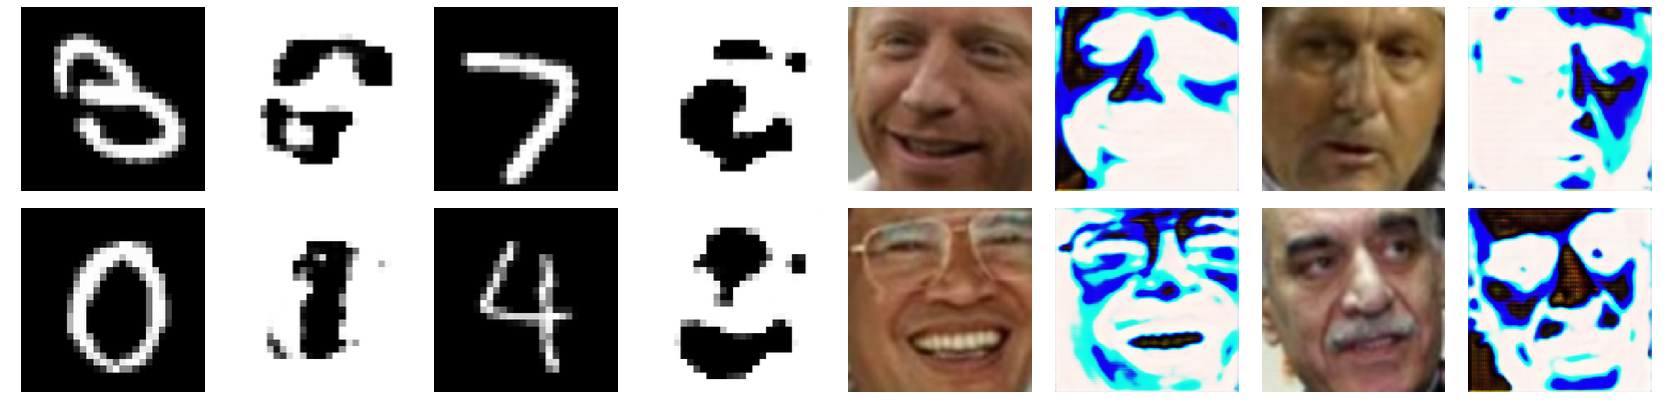
\includegraphics[width=0.7\textwidth]{images/preview.png}
}

\expandafter\def\expandafter\insertshorttitle\expandafter{%
  \insertshorttitle\hfill%
  \insertframenumber\,/\,\inserttotalframenumber}

\AtBeginSection[]{
  \begin{frame}
  \vfill
  \centering
  \begin{beamercolorbox}[sep=8pt,center,shadow=true,rounded=true]{title}
    \usebeamerfont{title}\insertsectionhead\par%
  \end{beamercolorbox}
  \vfill
  \end{frame}
}

\begin{document}
	\frame {
		\titlepage
	}
 
	\begin{frame}{План}
        \tableofcontents
    \end{frame}
	 
	\section{Вступ}
	\subsection{Supervised Learning}
	\begin{frame}{Формулювання задачі}	
		\begin{columns}
            % -- Description --
            \begin{column}{0.6\textwidth}
                Зазвичай, на вхід подається набір даних виду:
                \begin{equation*}
                    \mathcal{D} = \{(x_1,y_1),(x_2,y_2),\dots,(x_n,y_n)\},
                \end{equation*}
                
                де задача -- побудувати функцію $f$, що ``достатньо точно'' відображає $x_i$ на $y_i$ (\textit{Supervised Learning}).
    
                \begin{exampleblock}{Приклад}
                    Розпізнавання цифри з зображення. $x_i$ (вхід) -- зображення, $y_i$ (вихід) -- цифра від $0$ до $9$.
                \end{exampleblock}
            \end{column}

            % -- Figure --
            \begin{column}{0.4\textwidth}
                \begin{figure}
                \centering
                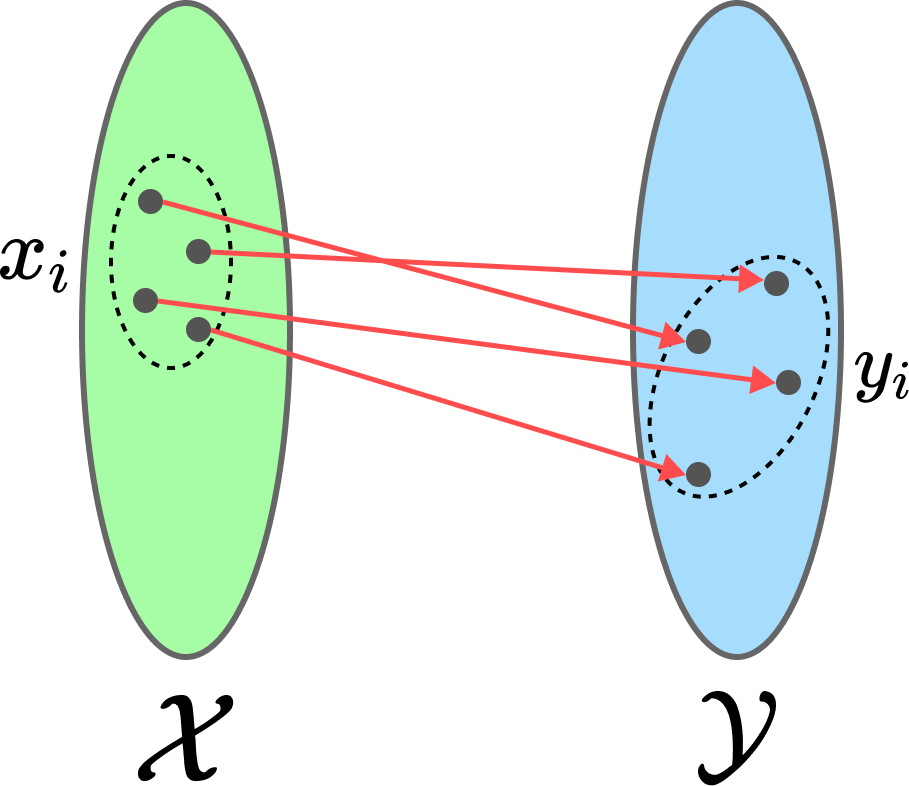
\includegraphics[width=1\textwidth]{images/mapping.png}
                \caption{Вхідний набір данних $\mathcal{D}$ -- послідовність пар виду $x_i \mapsto y_i$.}
                \end{figure}
            \end{column}
        \end{columns}
	\end{frame}

    \begin{frame}{Приклад: MNIST}	
        \begin{figure}
            \centering
            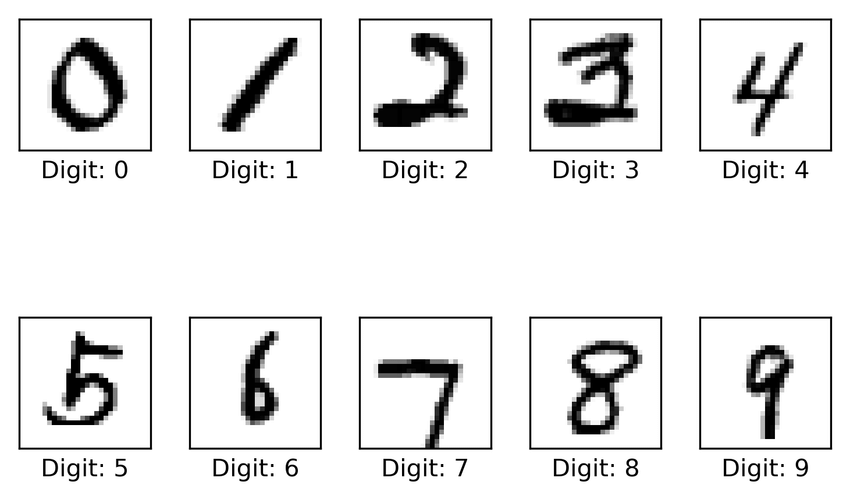
\includegraphics[width=0.8\textwidth]{images/mnist.png}
            \caption{Розпізнавання цифр. Набір данних MNIST -- найбільш популярний вибір для написання прототипів (\textit{Proof of Concept}).}
        \end{figure}
    \end{frame}

    \begin{frame}{Ефективність відображення}	
        \begin{exampleblock}{Питання}
            Як оцінити, що задана функція $f$ є ``гарною'' або ``поганою''?
        \end{exampleblock}
        
        \begin{figure}
            \centering
            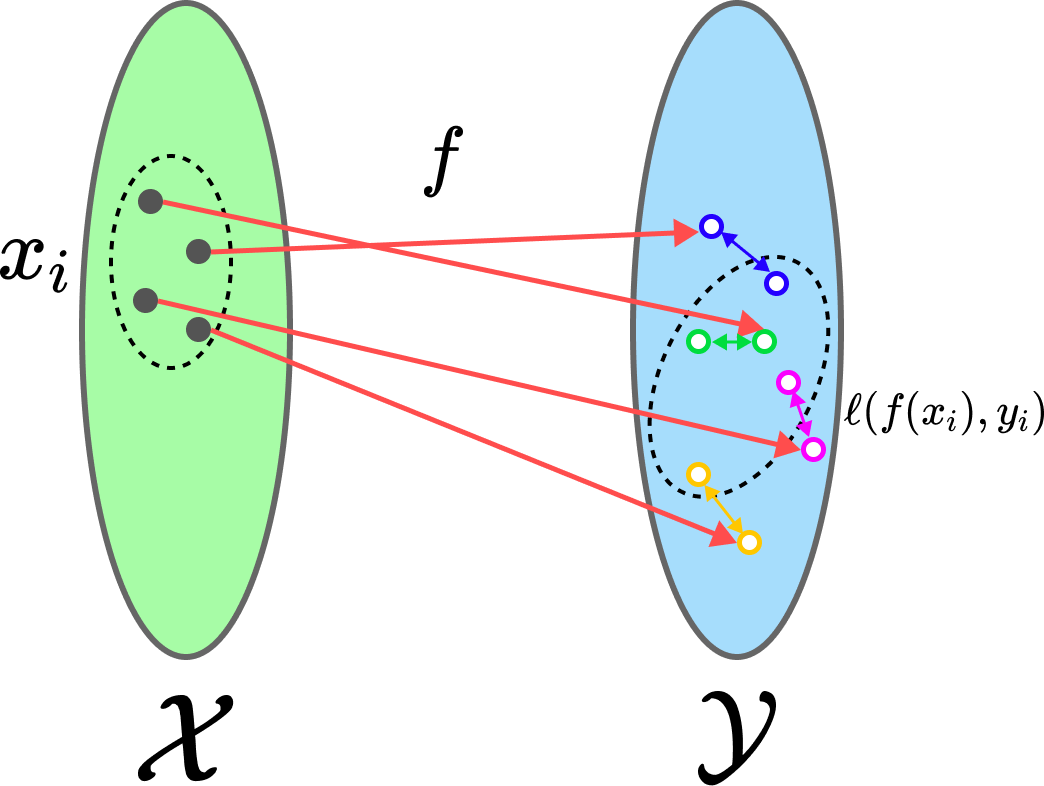
\includegraphics[width=0.6\textwidth]{images/loss.png}
            \caption{$f(x_i)$ ``промахнулось'' і дало відхилення від $y_i$ -- що далі?}
        \end{figure}
	\end{frame}

    \begin{frame}{Функція втрати}
        \textcolor{ForestGreen}{\cmark} Введемо втрату $\ell$ -- міра відстані між передбаченням $\hat{\mathbf{y}}=f(\mathbf{x})$ та фактичним значенням $\mathbf{y}$.
    
        \begin{exampleblock}{Приклад функції втрати}
            Якщо вихідне значення -- вектор, то можна покласти $\ell(\mathbf{y},\hat{\mathbf{y}}) := \text{відстань}(\mathbf{y},\hat{\mathbf{y}})$.
        \end{exampleblock}
    
        \begin{figure}
            \centering
            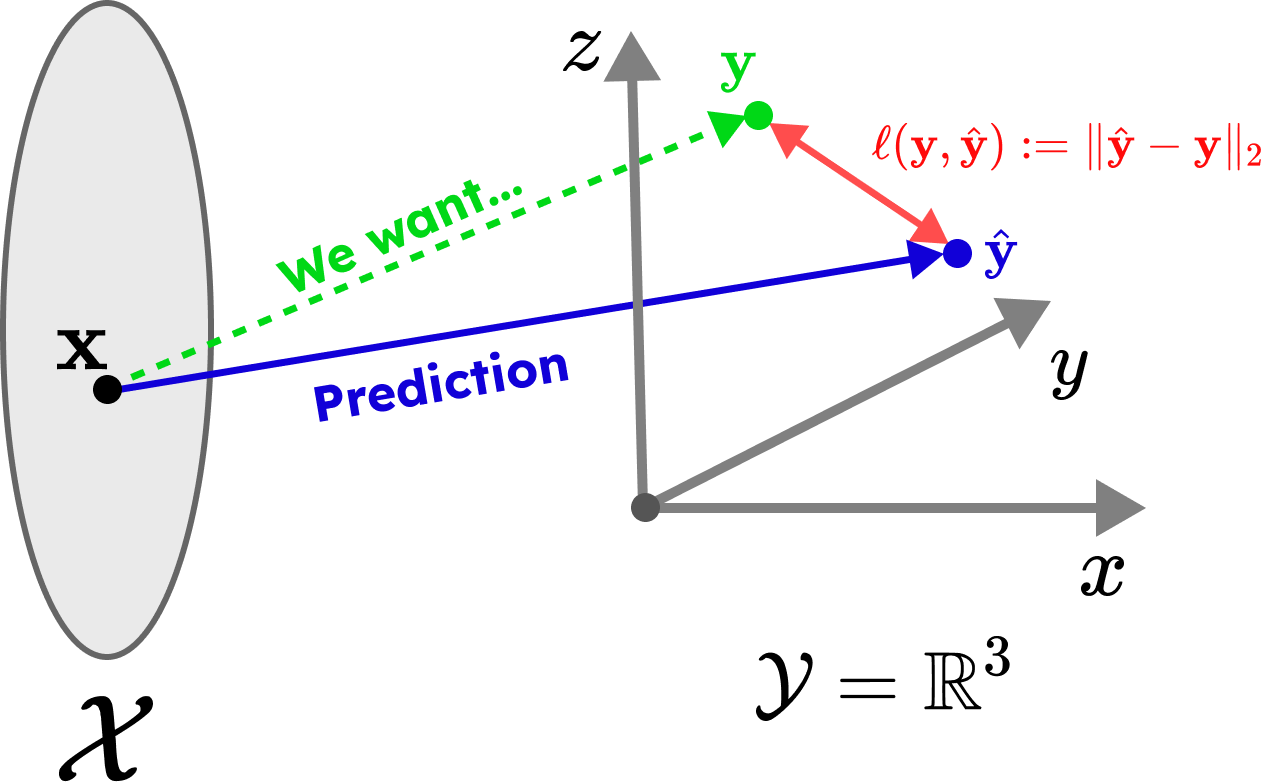
\includegraphics[width=0.5\textwidth]{images/loss_R3.png}
            \caption{Для $\mathcal{Y}=\mathbb{R}^3$ беремо Евклідову відстань для $\ell$.}
        \end{figure}
	\end{frame}
 
    \begin{frame}{Оптимізаційна задача}
        \begin{columns}
            % -- Text Column --
            \begin{column}{0.5\textwidth}
                Нехай функція $f(\star;\theta)$ параметризована набором параметрів $\theta$. 

                \begin{exampleblock}{Приклад параметризації}
                    Наприклад, нехай ми шукаємо
                    \begin{equation*}
                        f(x) = a x + b,
                    \end{equation*}
                    де $\theta=(a,b)$
                \end{exampleblock}

                Задача -- мінімізувати втрату $\ell(f(x_i),y_i)$.
            \end{column}
            % -- Figure --
            \begin{column}{0.5\textwidth}
                \begin{figure}
                    \centering
                    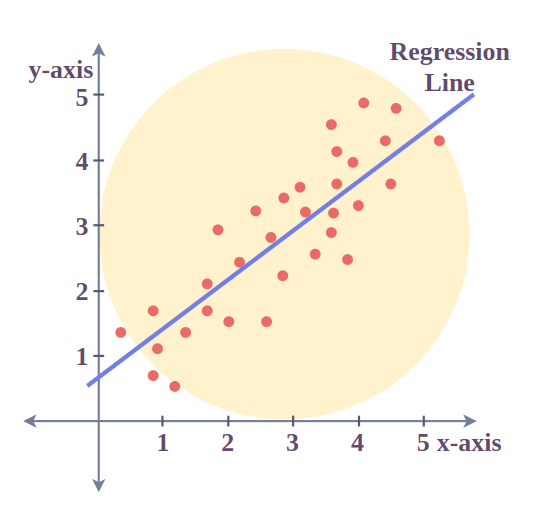
\includegraphics[width=\textwidth]{images/regression.png}
                    \caption{Підбираємо пряму, що проходить максимально близько до інших точок.}
                \end{figure}
            \end{column}
        \end{columns}
    \end{frame}
    
    \subsection{Dense Neural Networks}
    \begin{frame}{Повнозв'язні нейронні мережі (Dense Neural Networks)}
        Будуємо функцію, що на вхід приймає вектор довжини $n_{\text{in}}$, на вихід видає вектор довжини $n_{\text{out}}$, а також параметризована матрицями ваг та зсувами (bias).
        \begin{figure}
            \centering
            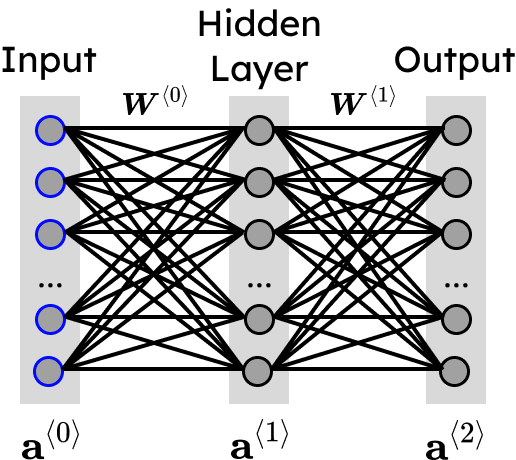
\includegraphics[width=0.45\textwidth]{images/flat_network.png}
            \caption{Приклад повнозв'язаної нейронної мережі з трьома шарами.}
        \end{figure}
    \end{frame}

    \begin{frame}{Вхідні нейрони}
        \begin{block}{Що таке нейрон?}
            Нейрон -- структурна одиниця нейронної мережі. По своїй суті -- вершина, що містить число -- активацію.
        \end{block}
    
        \begin{figure}
            \centering
            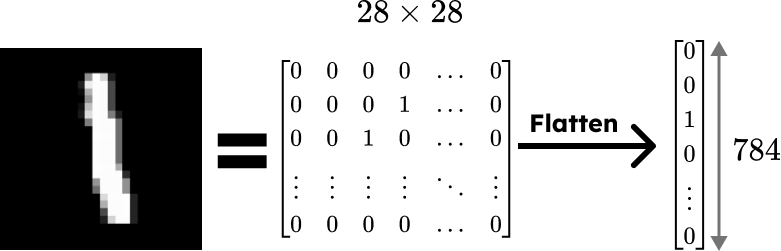
\includegraphics[width=0.9\textwidth]{images/flatten.png}
            \caption{Нейрони у першому шарі. Матрицю зображення перетворюємо у плоский вектор.}
        \end{figure}
    \end{frame}
    \begin{frame}{Forward Propagation}
        \begin{figure}
            \centering
            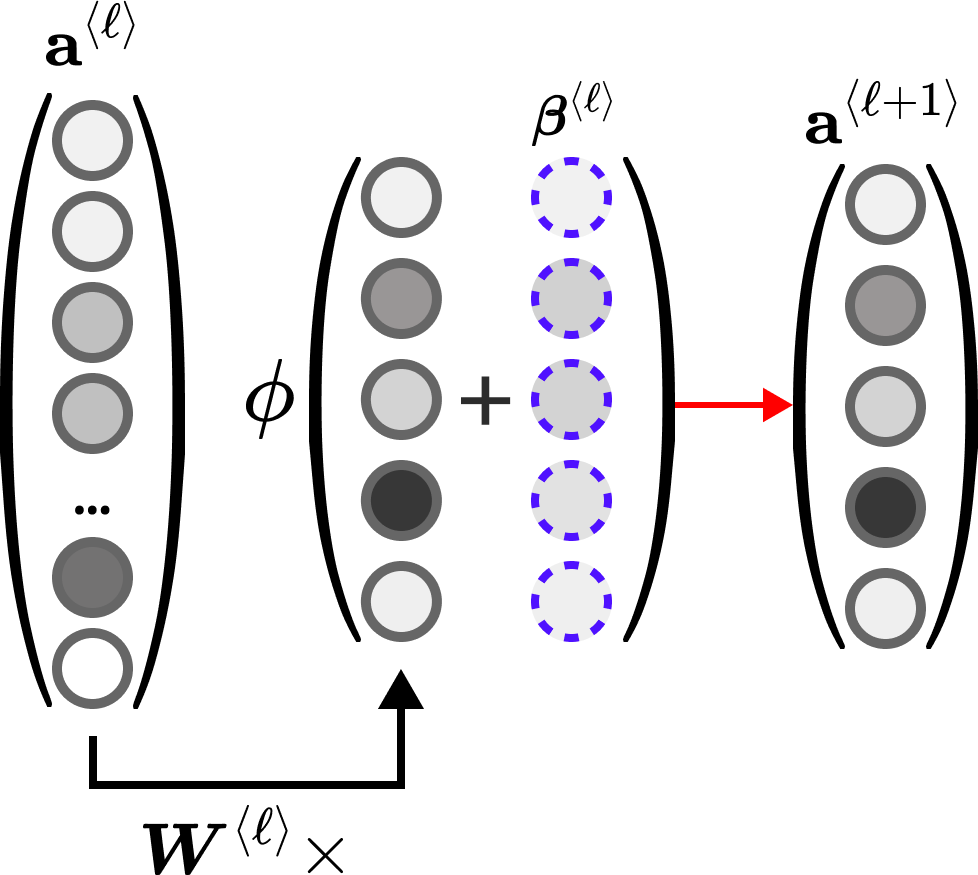
\includegraphics[width=0.5\textwidth]{images/forward_prop.png}
            \caption{Пряме поширення. Спочатку знаходимо матричний добуток, додаємо зсув і накладаємо нелінійну функцію.}
        \end{figure}
    \end{frame}

    \begin{frame}{Пряме поширення: обрахунок втрати}

    \begin{figure}
        \centering
        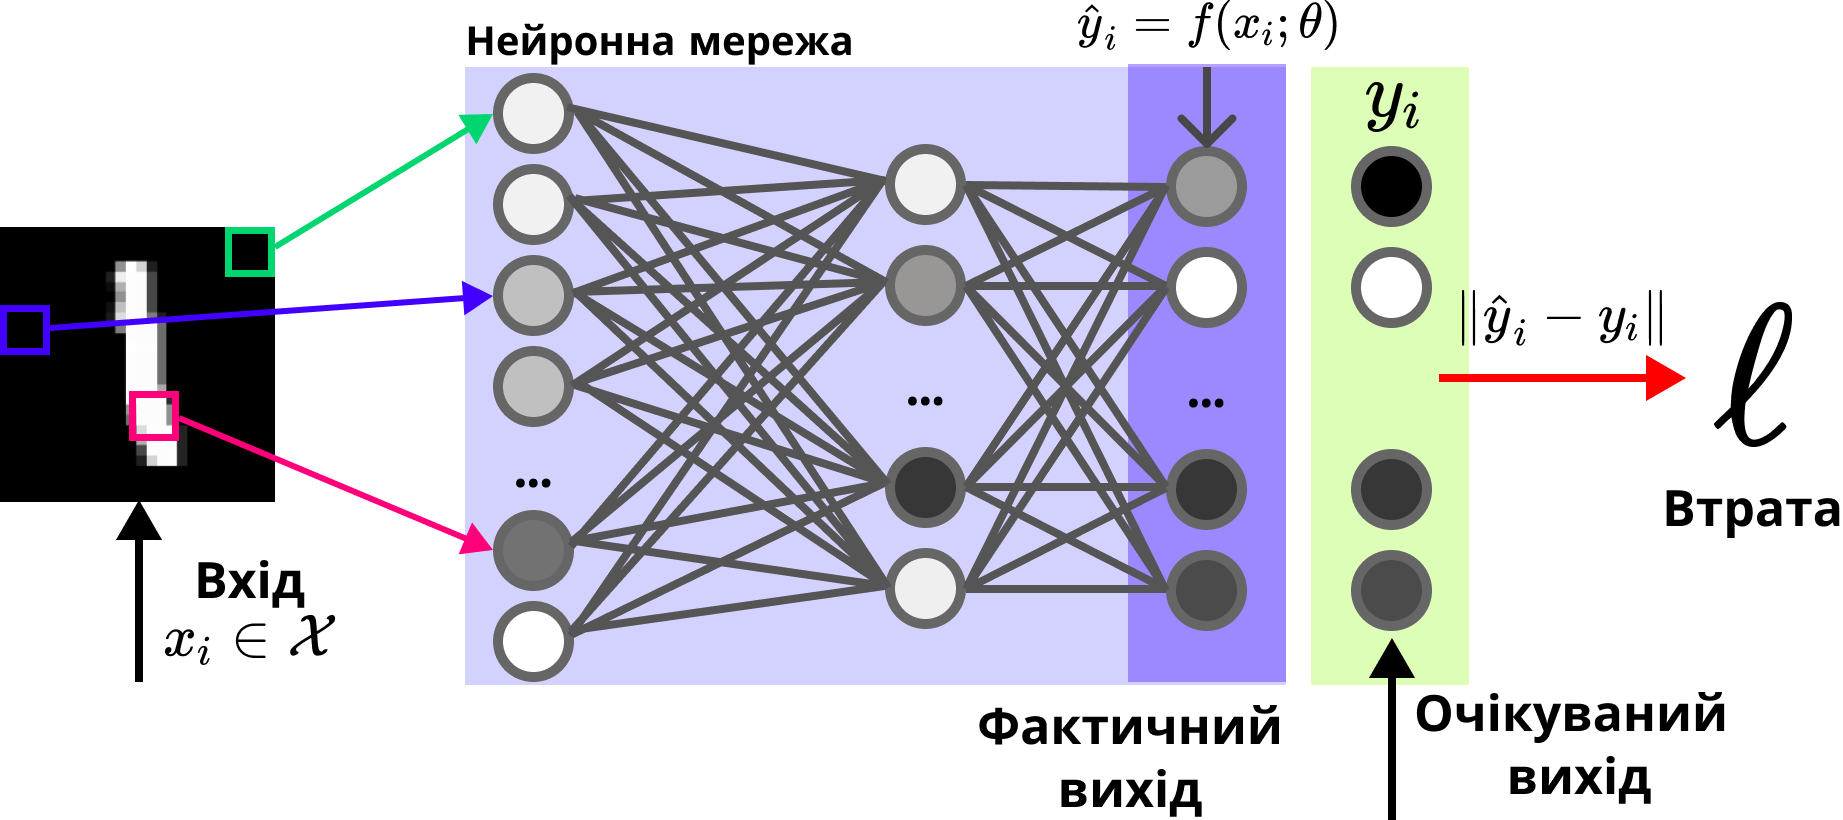
\includegraphics[width=\textwidth]{images/full_forward_prop.png}
        \caption{Пряме поширення: обрахунок значення втрати}
    \end{figure}

    \end{frame}

    \begin{frame}{Резюме}
        \begin{itemize}
            \item Нейронна мережа $f$ -- багатопараметризована функція.
            \item Dense нейронна мережа приймає вектор і ``випльовує'' також вектор.
            \item Маючи набір данних, ми намагаємося мінімізувати певну задану функцію $\ell$, підбираючи параметри у сімействі функцій.
        \end{itemize}    
	\end{frame}

    \subsection{Convolutional Neural Networks}
	\begin{frame}{Мотивація використання конволюційної нейронної мережі}
	    \begin{figure}
        \centering
            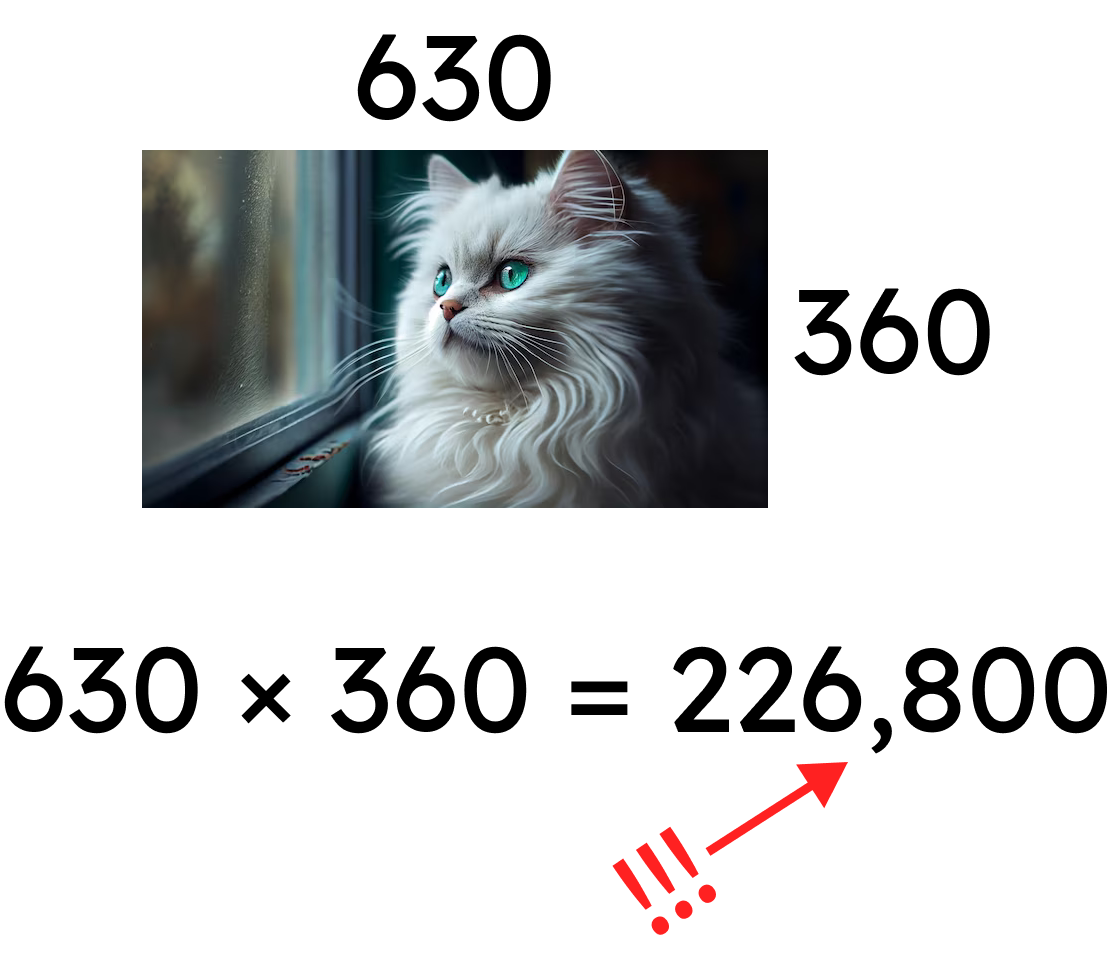
\includegraphics[width=0.73\textwidth]{images/cnn_motivation.png}
        \end{figure}
	\end{frame}
%     \begin{frame}[fragile] {Конволюційна операція}
%     \begin{figure}
%         \begin{tikzpicture}[mmat/.style={matrix of math nodes,column sep=-\pgflinewidth/2,
%    row sep=-\pgflinewidth/2,cells={nodes={draw,inner sep=3pt,thin}},draw=####1,thick,inner sep=0pt},
%    mmat/.default=black,
%    node distance=0.3em]
%  \matrix[mmat](mat1){
%          0 & 1 & 1 & 1 & 0 & 0 & 0 \\ 
%          0 & 0 & 1 & 1 & 1 & 0 & 0 \\ 
%          0 & 0 & 0 & 1 & 1 & 1 & 0 \\ 
%          0 & 0 & 0 & 1 & 1 & 0 & 0 \\ 
%          0 & 0 & 1 & 1 & 0 & 0 & 0 \\ 
%          0 & 1 & 1 & 0 & 0 & 0 & 0 \\ 
%          0 & 1 & 0 & 0 & 0 & 0 & 0 \\ 
%          };
%  \def\myarray{{1,0,1},{0,1,0},{1,0,1}}       
%  \foreach \X in {0,1,2}
%  {\foreach \Y in {0,1,2}
%   {\pgfmathsetmacro{\myentry}{{\myarray}[\Y][\X]}
%   \path (mat1-\the\numexpr\Y+1\relax-\the\numexpr\X+4\relax.south east)
%   node[anchor=south east,blue,scale=0.3,inner sep=1.2pt]{$\times\myentry$};
%   }}         
%  \node[fit=(mat1-1-4)(mat1-3-6),inner sep=0pt,draw,red,thick,name path=fit](f1){};      
%  \node[right=of mat1] (mul) {$*$};      
%  \matrix[mmat=blue,fill=blue!20,right=of mul,name path=mat2](mat2){    
%      1 & 0 & 1 \\ 
%      0 & 1 & 0 \\ 
%      1 & 0 & 1 \\ };
%  \node[right=of mat2] (eq) {$=$};       
%  \matrix[mmat,right=of eq](mat3){    
%      1 & 4 & 3 & |[draw=green,thick,fill=green!20,alias=4]|4 & 1 \\ 
%      1 & 2 & 4 & 3 & 3 \\ 
%      1 & 2 & 3 & 4 & 1 \\ 
%      1 & 3 & 3 & 1 & 1 \\ 
%      3 & 3 & 1 & 1 & 0 \\ 
%  };
%  \foreach \Anchor in {south west,north west,south east,north east}
%  {\path[name path=test] (f1.\Anchor) -- (mat2.\Anchor);
%  \draw[blue,densely dotted,name intersections={of=test and fit,total=\t}]
%  \ifnum\t>0 (intersection-\t) -- (mat2.\Anchor) \else
%   (f1.\Anchor) -- (mat2.\Anchor)\fi;
%  \path[name path=test2]  (4.\Anchor) -- (mat2.\Anchor);  
%  \draw[green,densely dotted,name intersections={of=test2 and mat2,total=\tt}] 
%  \ifnum\tt>0 (intersection-1) -- (4.\Anchor) \else
%     (mat2.\Anchor) --  (4.\Anchor)\fi;
%     }
%         \path (mat1.south) node[below] {$X$}(mat2|-mat1.south)node[below] {$\mathcal{K}$}(mat3|-mat1.south) node[below]{$X*\mathcal{K}$};
%             \begin{scope}[on background layer]
%                 \fill[red!20] (f1.north west) rectangle (f1.south east);
%             \end{scope}
%         \end{tikzpicture}
%         \caption{Механізм знаходження конволюції $X*\mathcal{K}$ для $\mathcal{K} \in \mathbb{R}^{3 \times 3}$ та $X \in \mathbb{R}^{7 \times 7}$.}
%     \end{figure}
%     \end{frame}

    \begin{frame}[fragile]{Фільтри Собеля}
        \begin{tikzpicture}
            \node[anchor=center,inner sep=0](raw1) at (0,0) {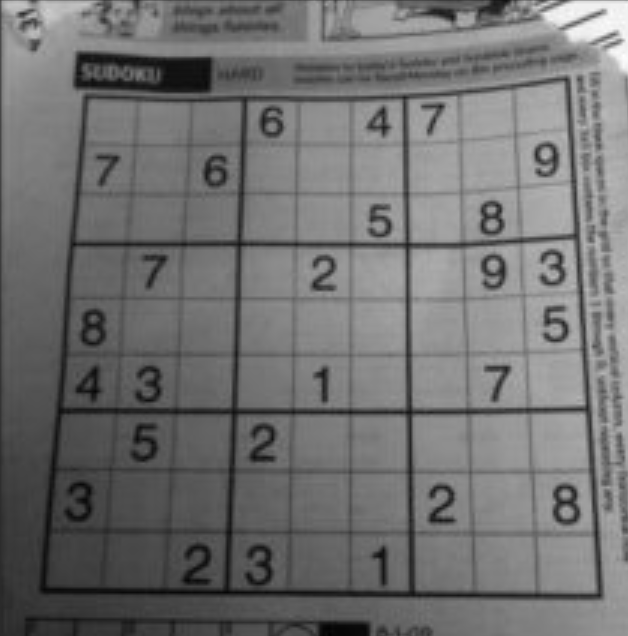
\includegraphics[width=0.3\textwidth]{images/raw.png}};
            \node[anchor=center,inner sep=0] at (2.15,-3.3) {$*$};
            \node[anchor=center,inner sep=0] at (5.8,-3.3) {$=$};
            \node[anchor=center,inner sep=0](sobel_x) at (4,0) {$\underbrace{\begin{bmatrix}
                +1 & 0 & -1 \\
                +2 & 0 & -2 \\
                +1 & 0 & -1
            \end{bmatrix}}_{\text{$x$ Sobel kernel}}$};
            \node[anchor=center,inner sep=0](img_x) at (8,0) {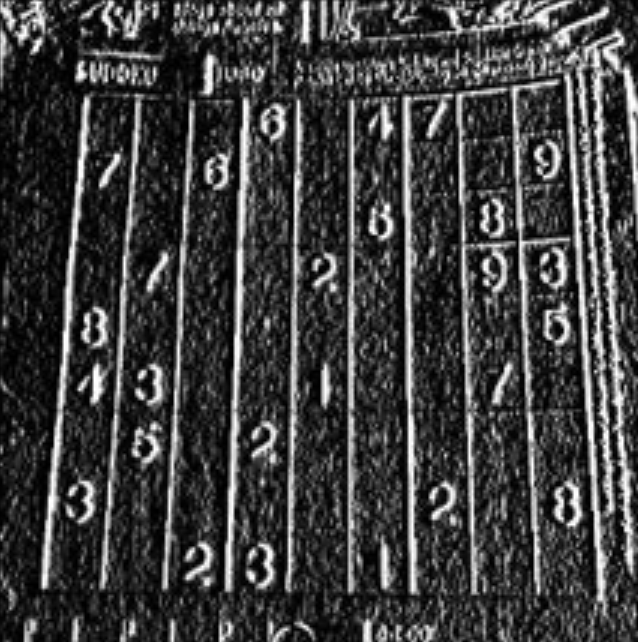
\includegraphics[width=0.3\textwidth]{images/sobel_x.png}};


            \node[anchor=center,inner sep=0](raw1) at (0,-3.5) {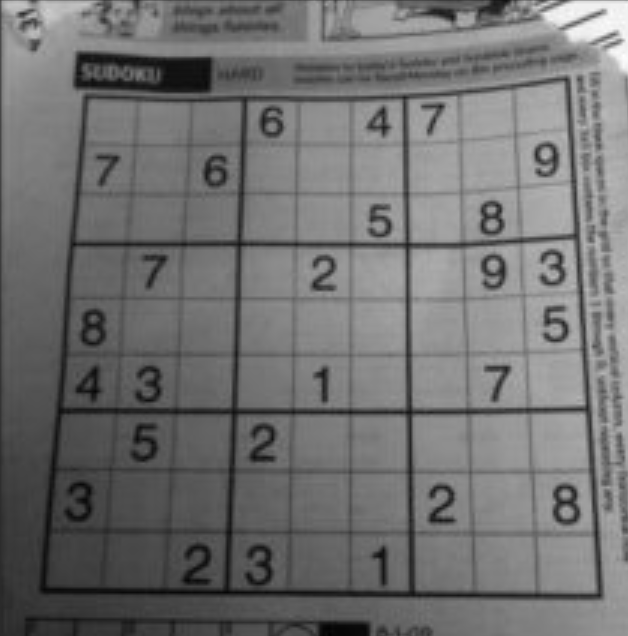
\includegraphics[width=0.3\textwidth]{images/raw.png}};
            \node[anchor=center,inner sep=0] at (2.15,0.2) {$*$};
            \node[anchor=center,inner sep=0] at (5.8,0.2) {$=$};
            \node[anchor=center,inner sep=0](sobel_x) at (4,-3.5) {$\underbrace{\begin{bmatrix}
                +1 & +2 & +1 \\
                0 & 0 & 0 \\
                -1 & -2 & -1
            \end{bmatrix}}_{\text{$y$ Sobel kernel}}$};
            \node[anchor=center,inner sep=0](img_x) at (8,-3.5) {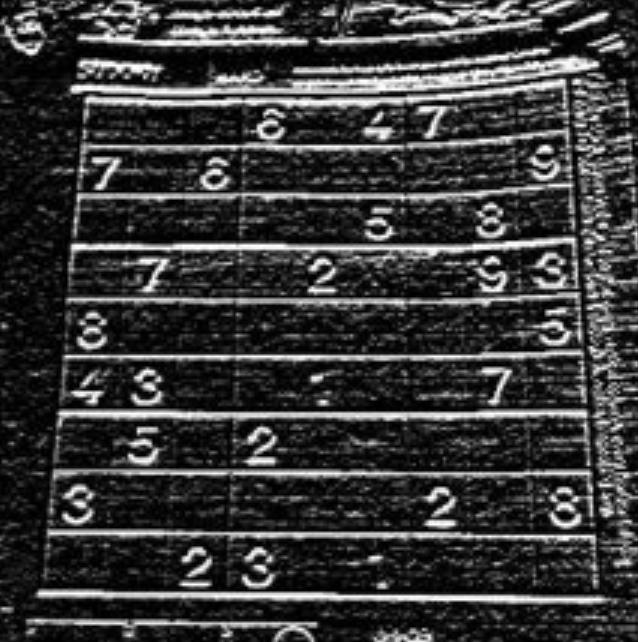
\includegraphics[width=0.3\textwidth]{images/sobel_y.png}};
        \end{tikzpicture}
    \end{frame}
    
    \begin{frame}{Конволюційний шар}
        \begin{itemize}
            \item Фільтр по зображенню $W \times H \times n_C$ з $n_C$ каналами -- це набір з $n_C$ фільтрів.
            \item Один набір -- один шар у вихідному ``об'ємі''. $n_f$ фільтрів дає вихід з $n_f$ каналами.
            \item Тренувальні параметри -- параметри фільтрів, зсуви (один на кожен фільтр), гіперпараметр -- активаційна функція.
        \end{itemize}        

        \begin{figure}
        \centering
            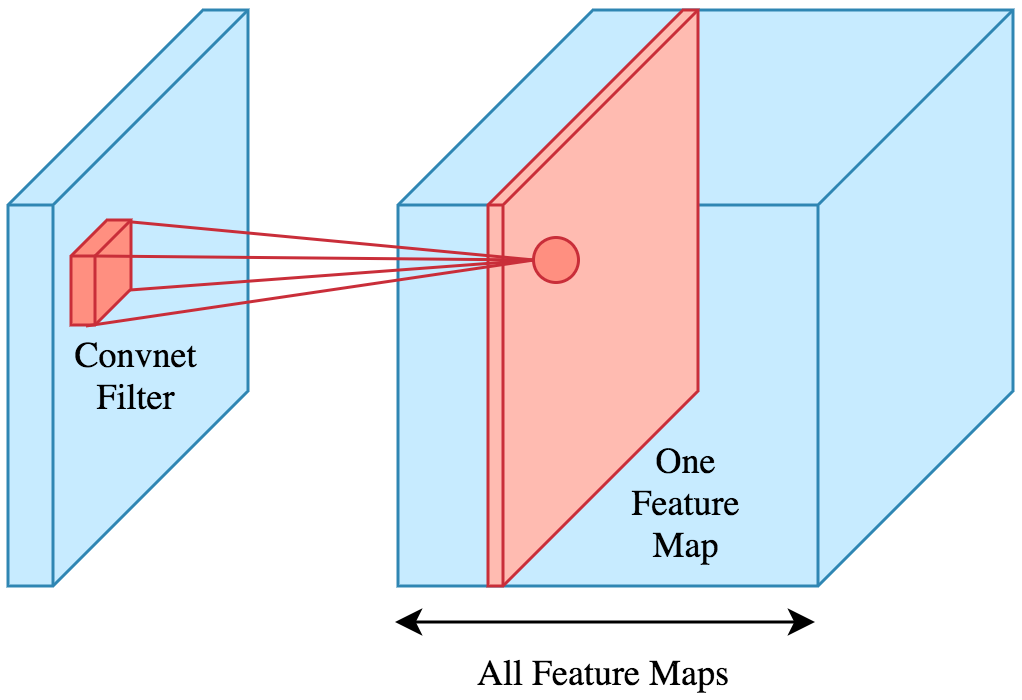
\includegraphics[width=0.55\textwidth]{images/cnn_volume.png}
        \end{figure}
    \end{frame}
	
    \begin{frame}{Max Pooling}
        1. Рухаємо $2\times 2 \times n_C$ фільтр по зображенню. 
        
        2. Взяти максимальний елемент на кожному каналі і записати у вихідне зображення.

        \textit{Навіщо це треба?} Ми зменьшуємо зображення в $4$ рази.

        \begin{figure}
        \centering
            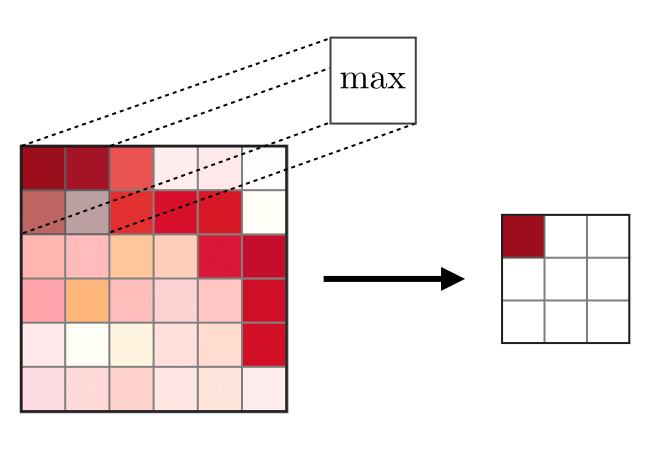
\includegraphics[width=0.55\textwidth]{images/max-pooling-a.png}
            \caption{Ілюстрація MaxPool шару. \scriptsize Зображення взято з \href{https://stanford.edu/~shervine/teaching/cs-230/cheatsheet-convolutional-neural-networks}{Afshine Amidi, Stanford CS 230 -- Deep Learning, CNN Cheatsheat}}
        \end{figure}
    \end{frame}

    \begin{frame}{Конволюційна нейронна мережа, підсумовуючи}
        1. Використовуємо конволюційні шари ($\mathsf{Conv2D}$).
        
        2. Зменьшуємо розмір зображення за допомогою \texttt{Conv2D} з $s=2$ або \texttt{MaxPool} шаром.
        
        3. Повторити, поки об'єм зображення не стане достатньо маленьким.

        4. Перевести у повнозв'язану нейронну мережу $\implies$ вихід.

        \begin{figure}
        \centering
            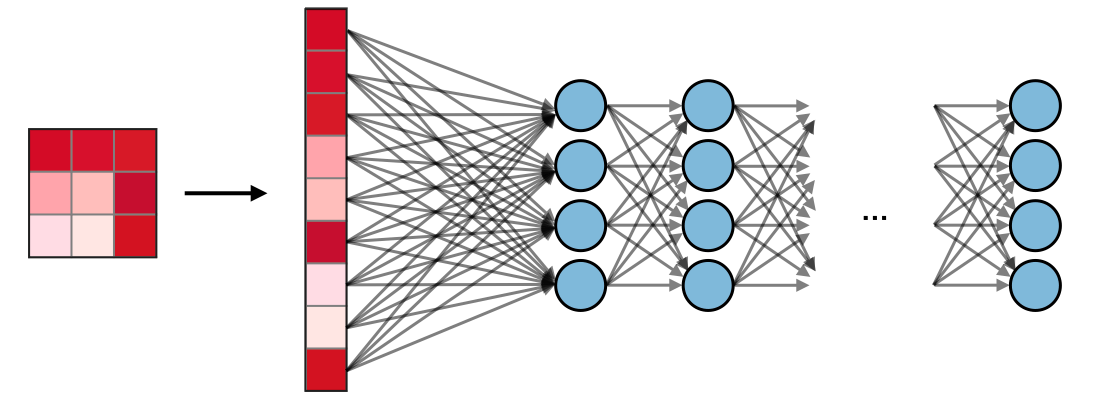
\includegraphics[width=0.8\textwidth]{images/cnn.png}
            \caption{Повнозв'язана нейронна мережа в кінці CNN. \scriptsize Зображення взято з \href{https://stanford.edu/~shervine/teaching/cs-230/cheatsheet-convolutional-neural-networks}{Afshine Amidi, Stanford CS 230 -- Deep Learning, CNN Cheatsheat}}
        \end{figure}
    \end{frame}

    \begin{frame}{Конволюційна нейронна мережа, підсумовуючи}
        \begin{figure}
        \centering
            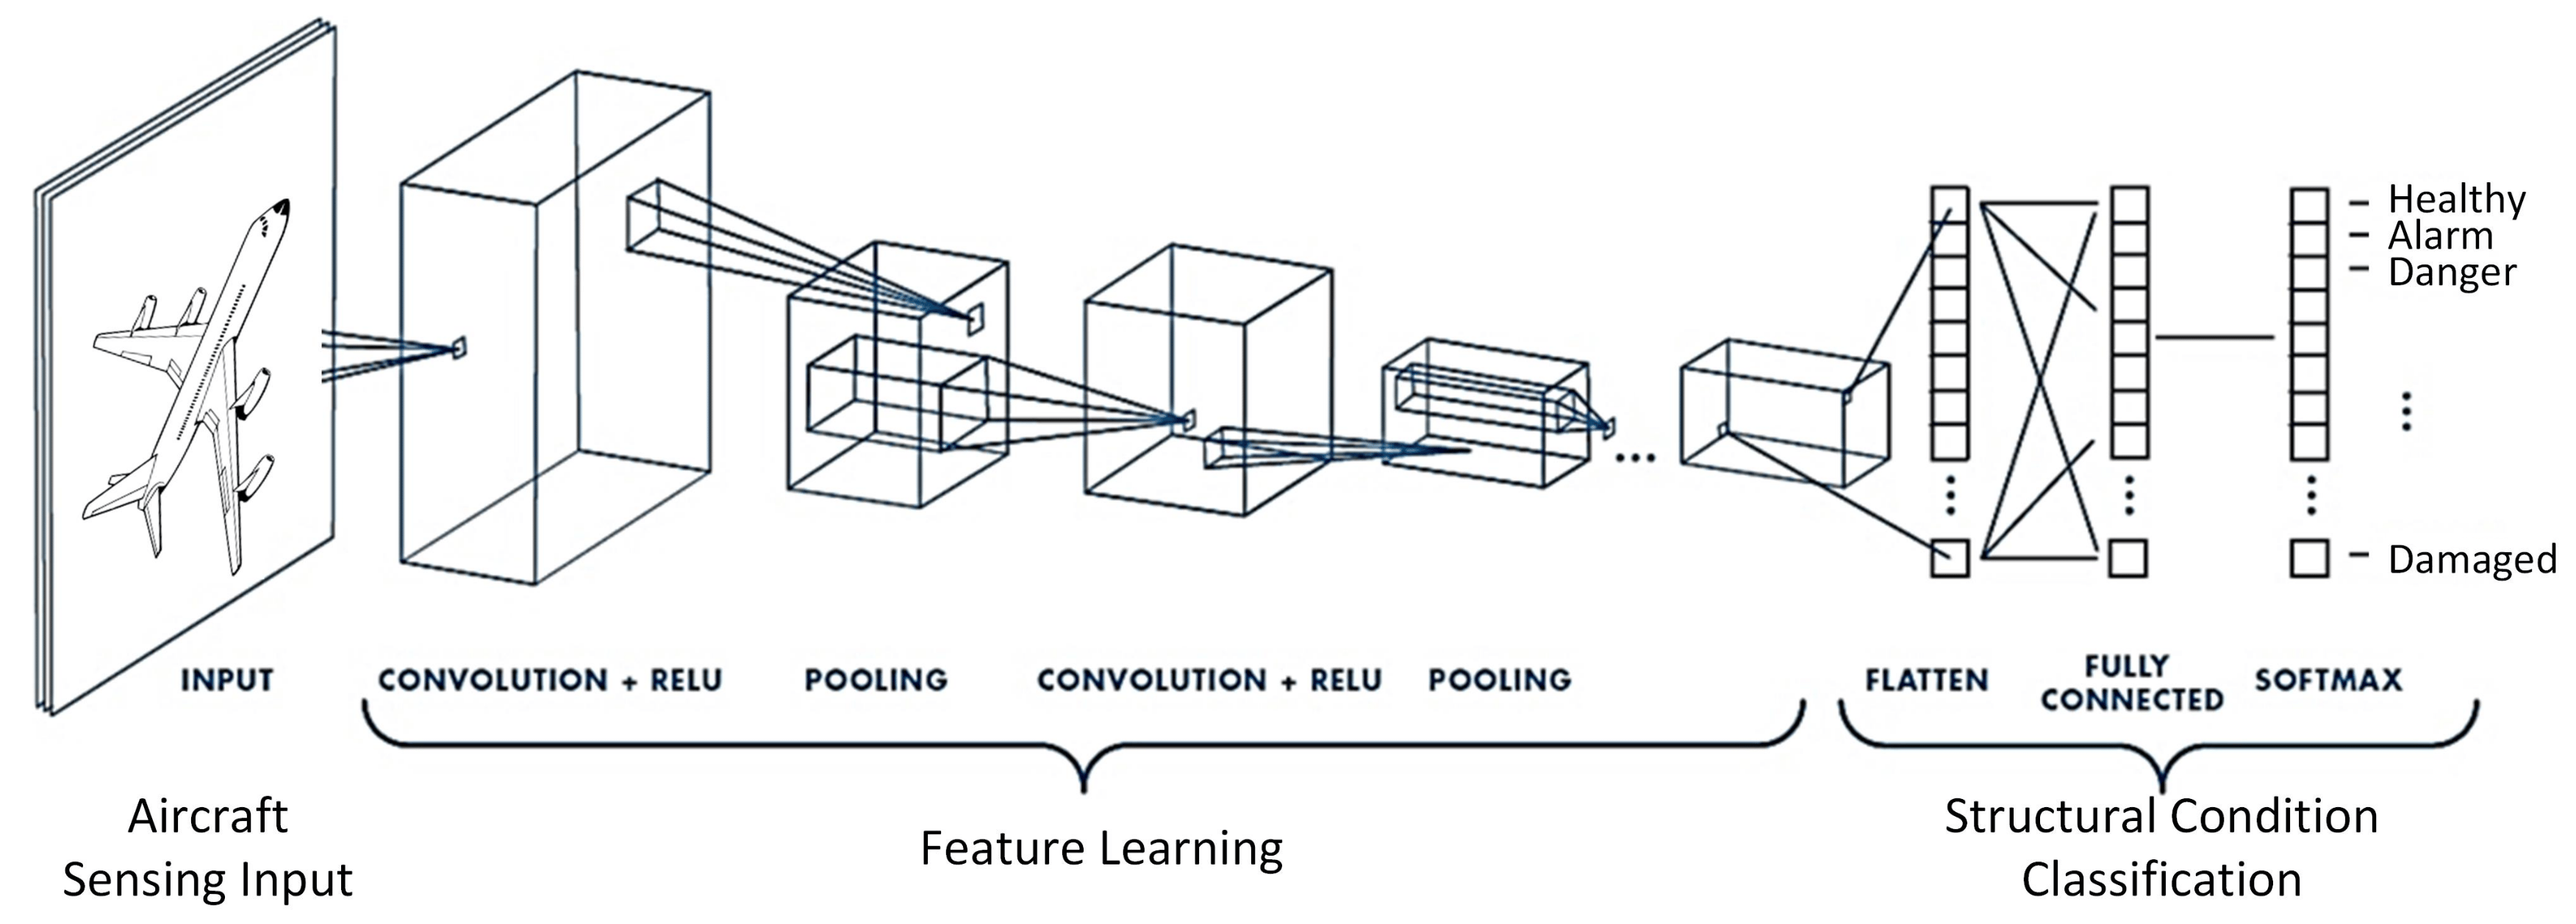
\includegraphics[width=\textwidth]{images/cnn_full.png}
            \caption{Повний вигляд конволюційної мережі. \scriptsize Зображення взято з роботи Iuliana Tabian et al. 2019. A Convolutional Neural Network for Impact Detection and Characterization of Complex Composite Structures.}
        \end{figure}
    \end{frame}

    \section{Deep Pattern Recognition}
    \subsection{Embedding Neural Network}
    \begin{frame}{Постановка задачі}
        Маючи два зображення $X,Y$, сказати чи відповідають вони одній людині чи ні.
        \begin{figure}
        \centering
            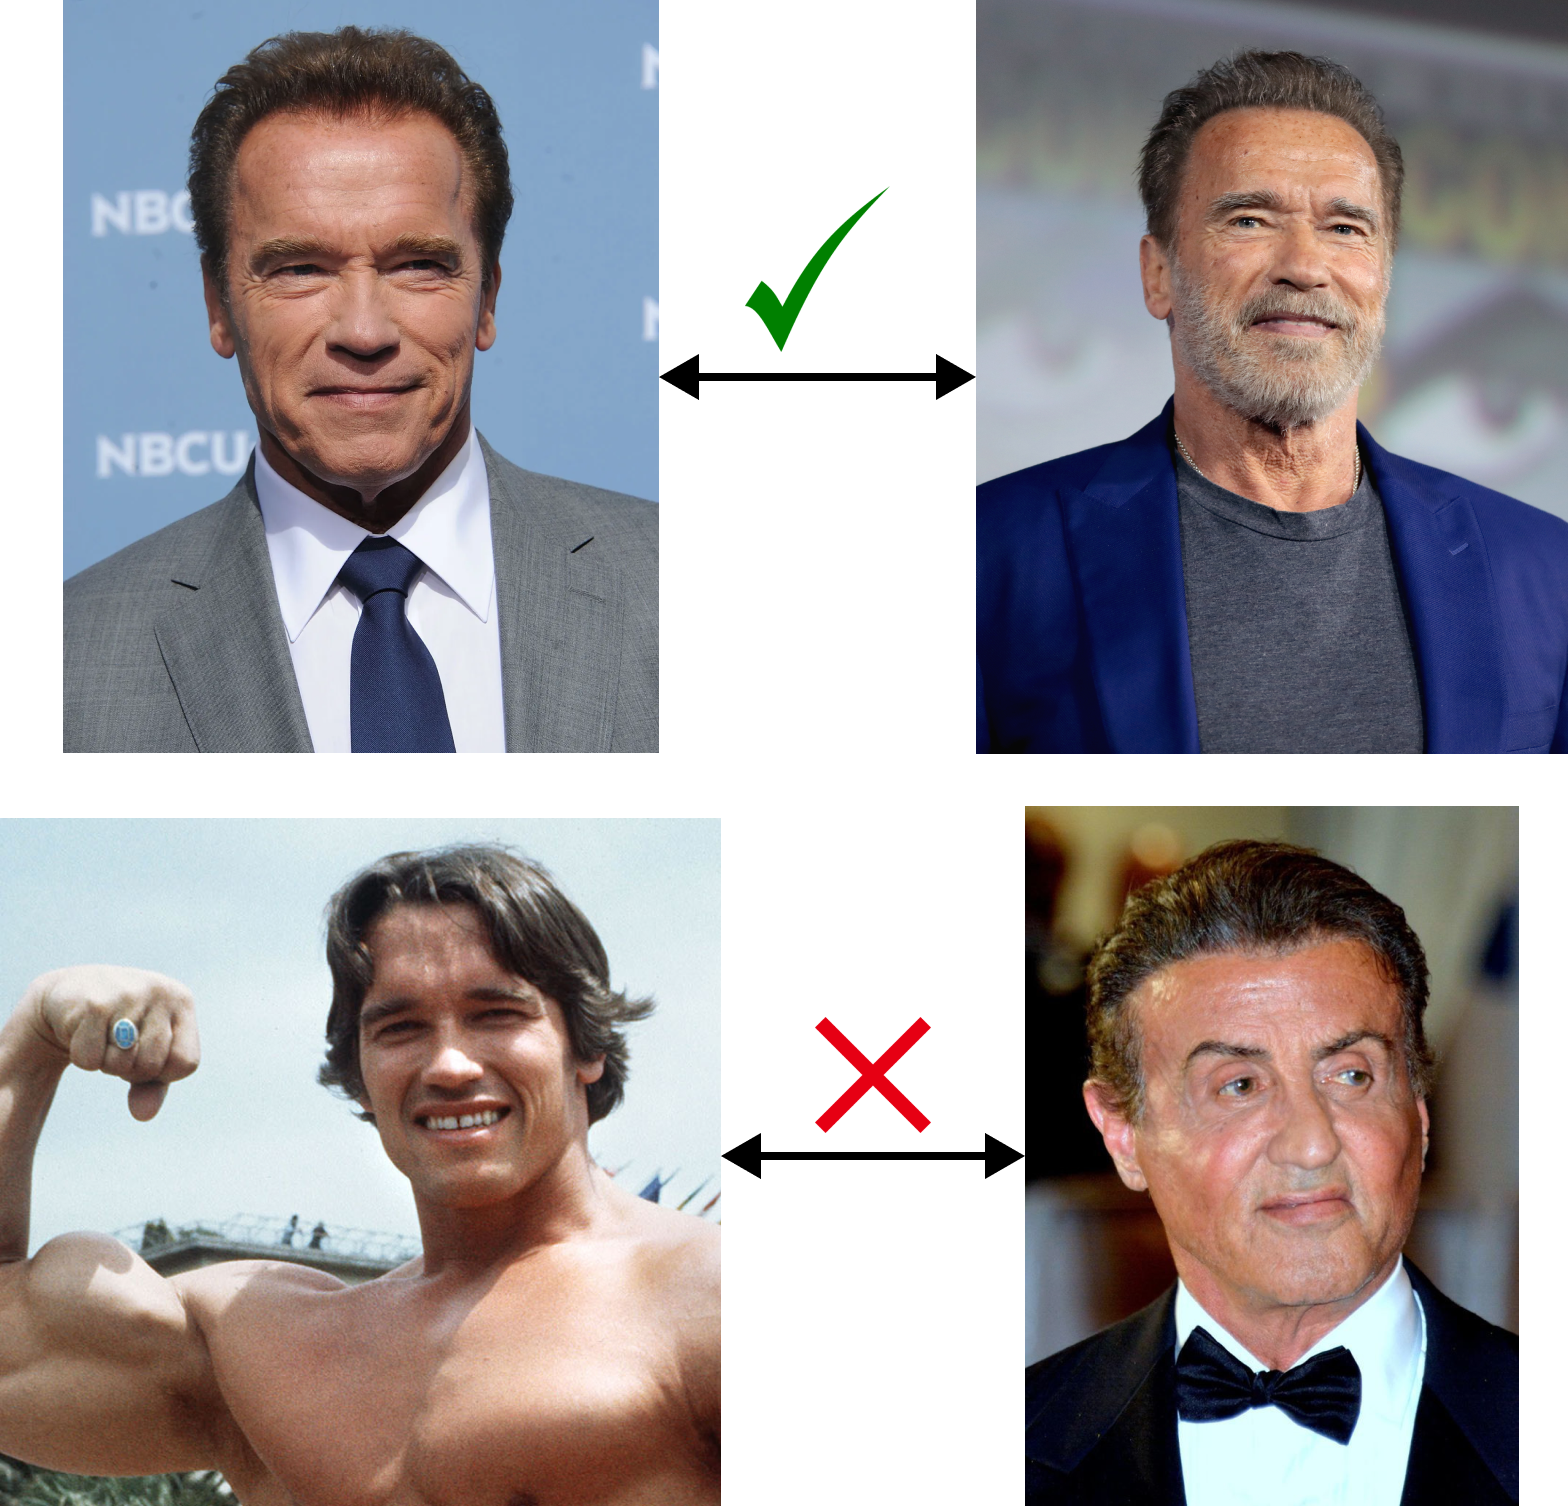
\includegraphics[width=0.57\textwidth]{images/face_comparison.png}
        \end{figure}
    \end{frame}

    \begin{frame}{Перша ідея}
        Нехай кожній людині відповідає номер. Тоді, будуємо класифікаційну нейронну мережу ($C$ -- кількість класів):
        \begin{equation*}
            \mathcal{F}: \mathsf{Image} \to \{1,\dots,C\}
        \end{equation*}
        \begin{figure}
        \centering
            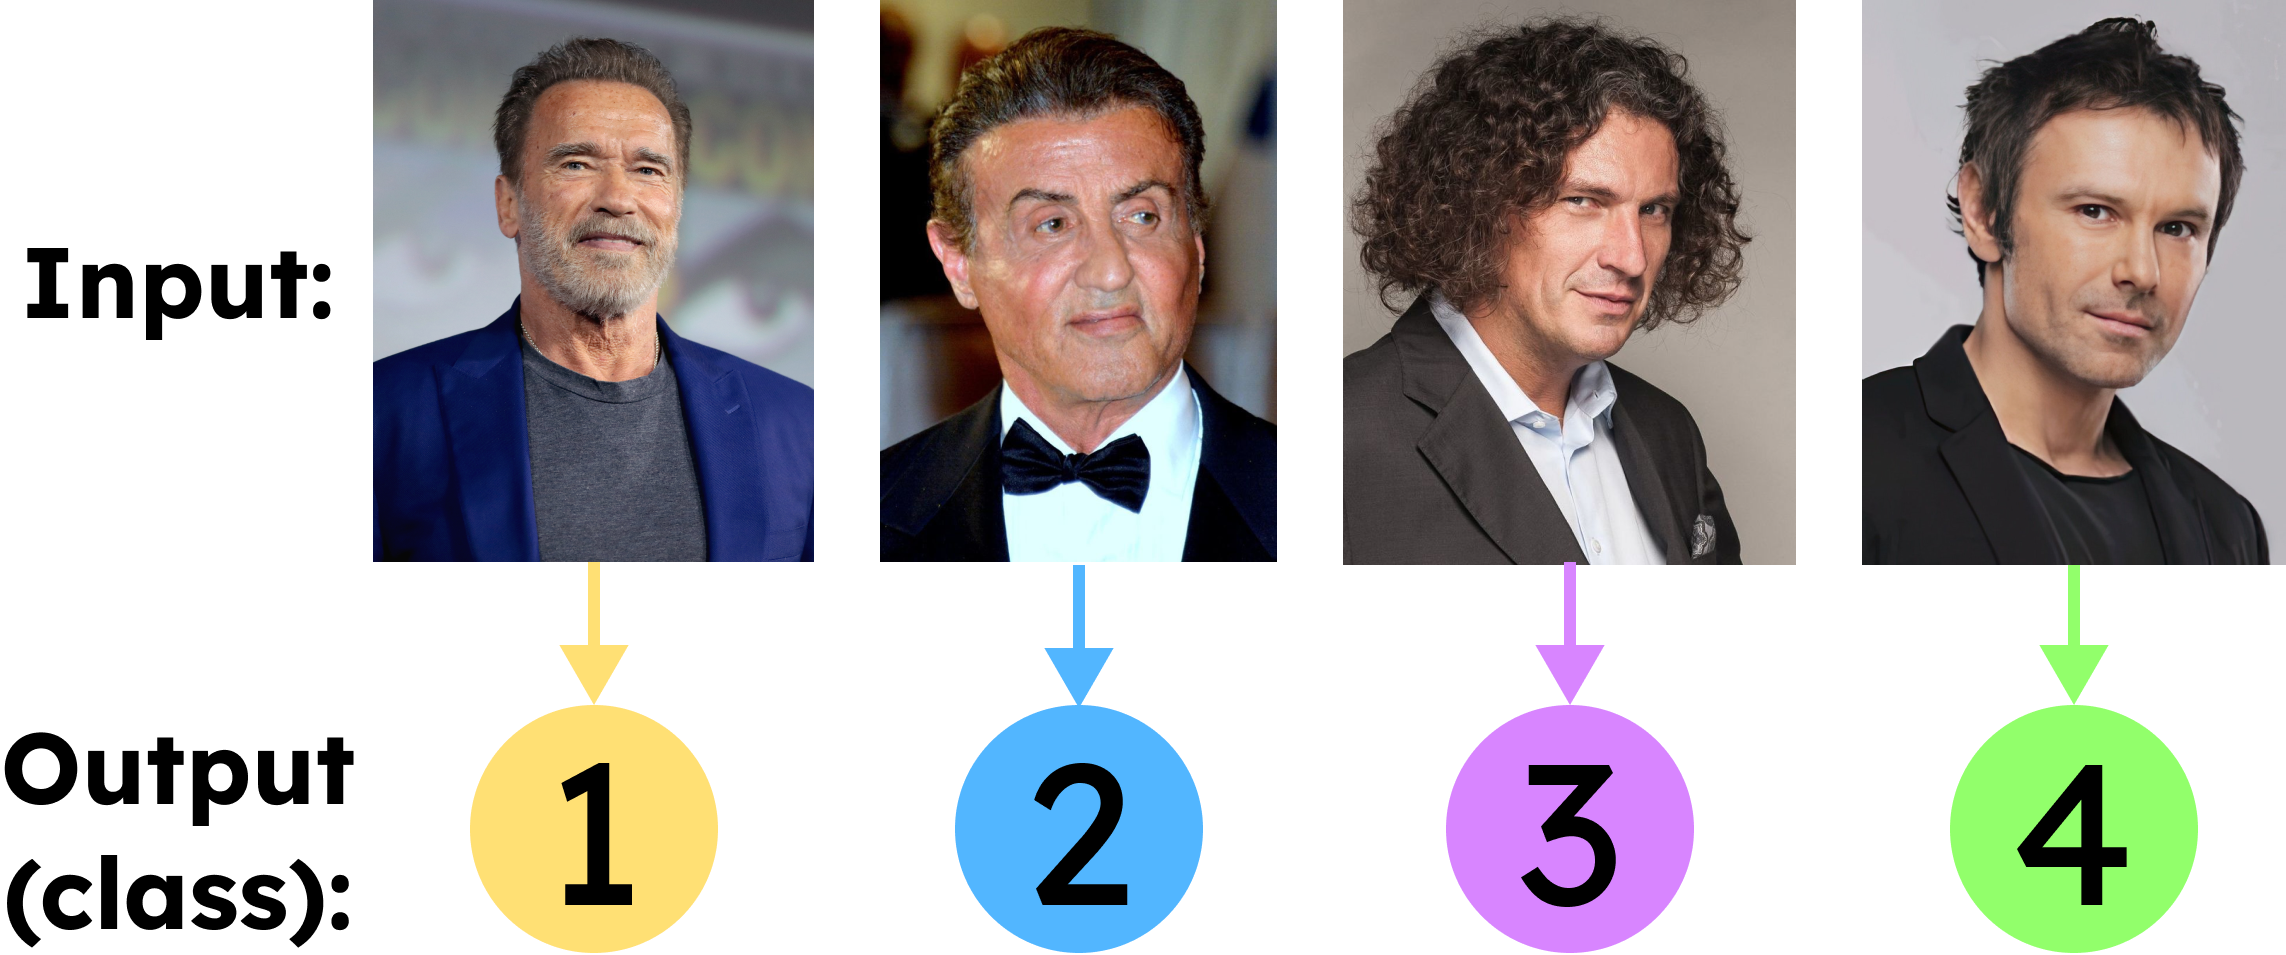
\includegraphics[width=0.7\textwidth]{images/recognition_classes.png}
            \caption{Даємо номер кожній людині і будуємо мультикласифікаційну модель.}
        \end{figure}
    \end{frame}

    \begin{frame}{Чому ні?}
        \begin{itemize}
            \item Людей м'яко кажучи багато -- близько $8.1$ млрд на момент написання цієї презентації :)
            \item Навіть маючи фіксований набір людей, потрібно більше 50-100 фотографій на людину (One-shot problem).
        \end{itemize}
        
        \begin{figure}
        \centering
            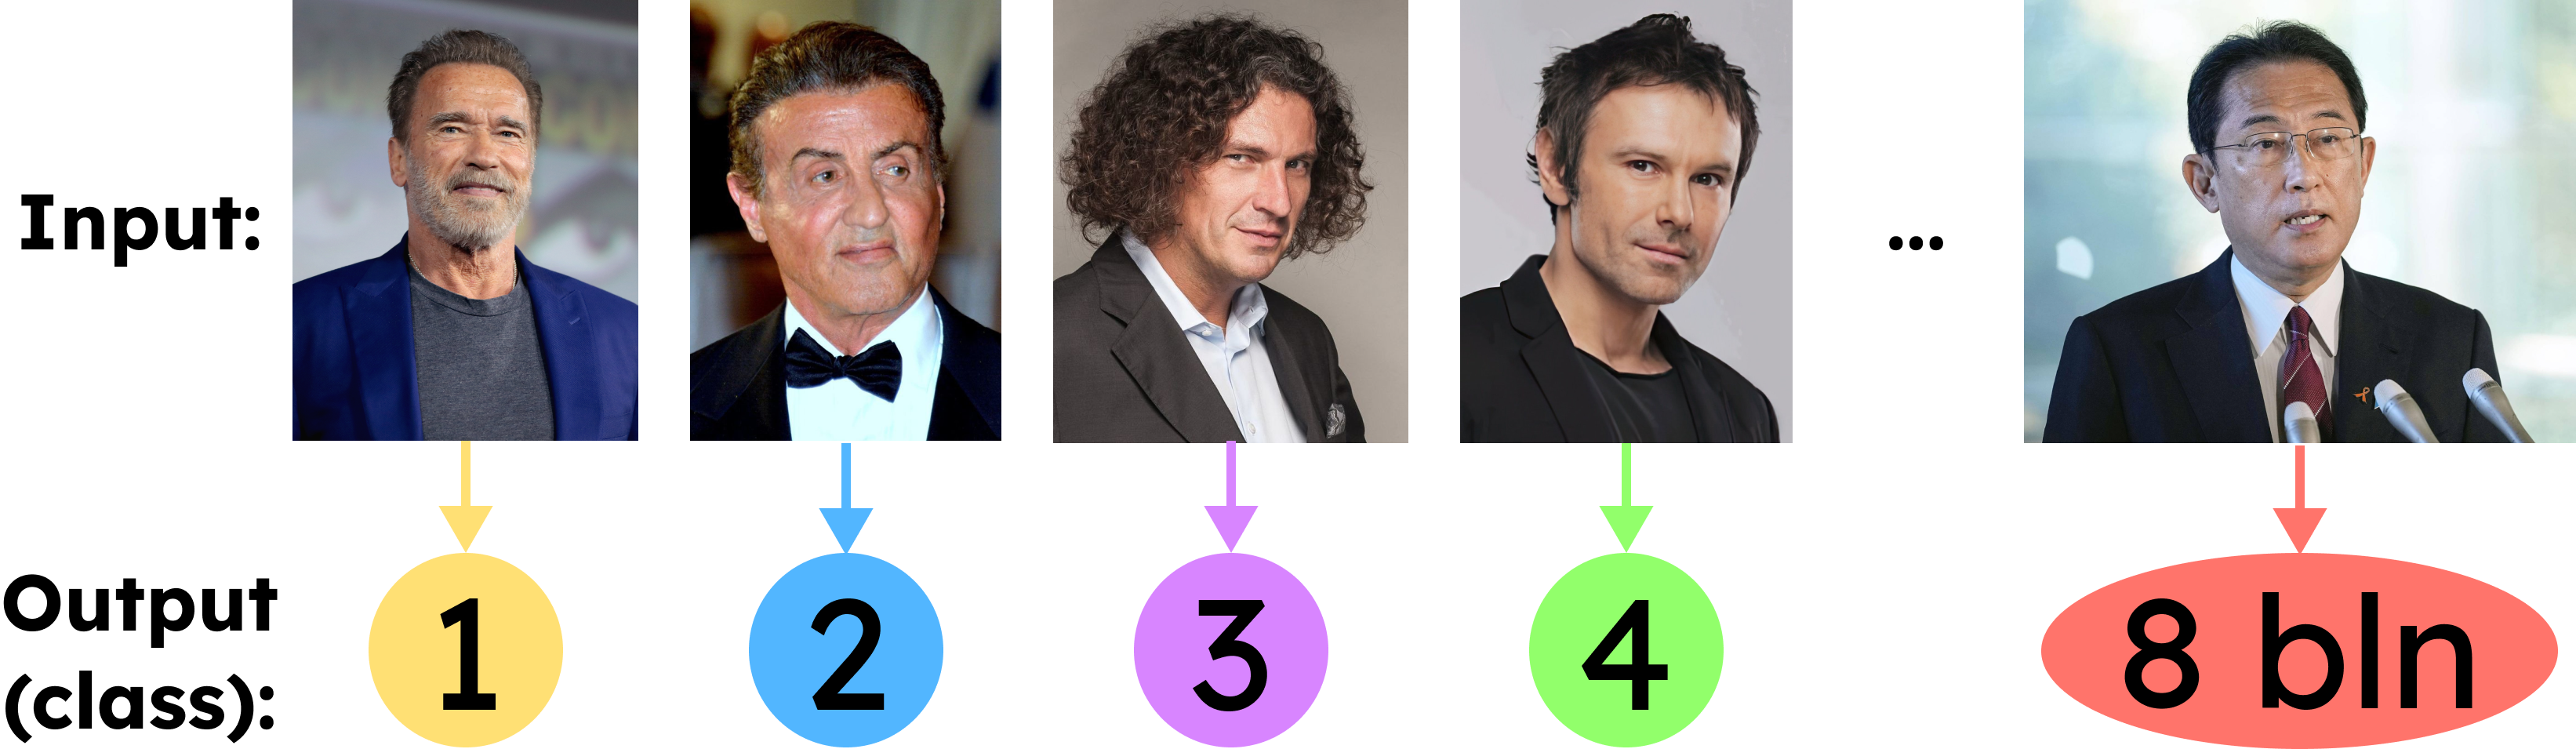
\includegraphics[width=0.7\textwidth]{images/too_many_people.png}
            \caption{Набір класів не є фіксованим, інакше нам доведеться зафіксувати 8+ млрд класів}
        \end{figure}
    \end{frame}

    \begin{frame}{Друга ідея: Embedding Neural Network}
        Будуємо $\mathcal{F}: \mathsf{Image} \to S^{m-1}$. Вперше запропоновано в Florian Schroff et al. ``FaceNet: A Unified Embedding for Face Recognition and Clustering''. 2015. 
        \begin{figure}
        \centering
            \includegraphics[width=0.4\textwidth]{images/hypersphere.png}
            \caption{Вихід функції (вектор фіч або ``embedding vector'') буде давати ``характеристику'' людини.}
        \end{figure}
    \end{frame}

    \begin{frame}{Embedding Neural Network: інтуїція}
        Приклад вектору фіч -- це набір відстаней між ключовими точками.
        \begin{figure}
        \centering
            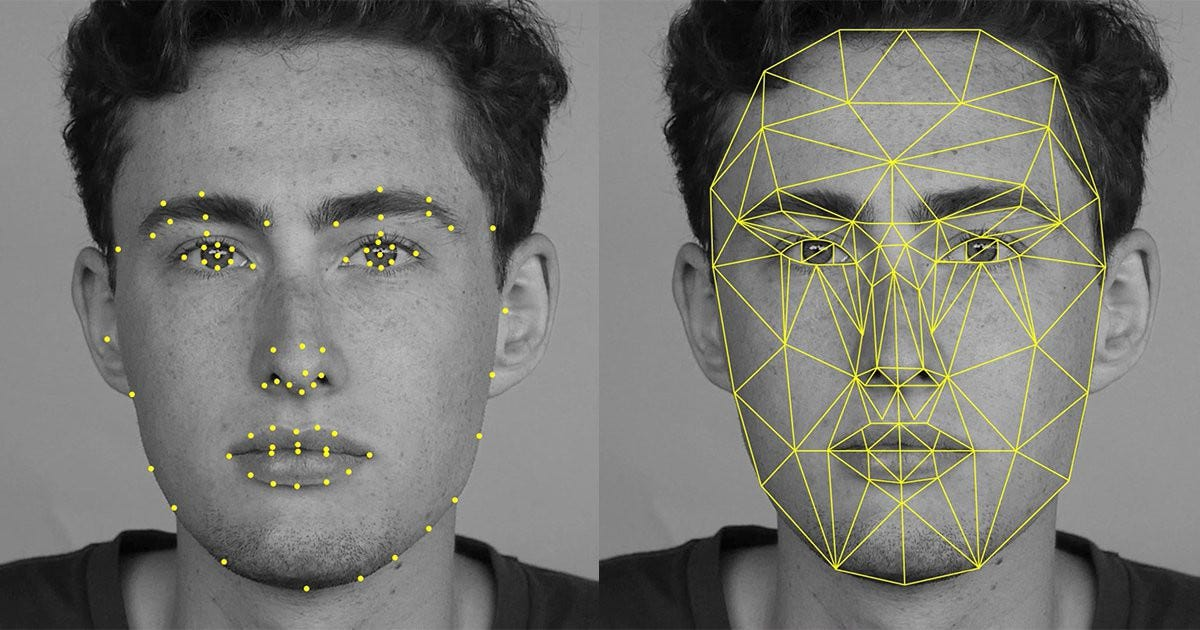
\includegraphics[width=0.75\textwidth]{images/keypoints.jpg}
            \caption{Ключові точки на обличчі.}
        \end{figure}
    \end{frame}

    \begin{frame}{Ілюстрація роботи Embedding нейронної мережі}
        \begin{exampleblock}{Приклад}
            Нехай на вхід ми отримали зображення $X,Y,Z$ і для $m=3$ ми отримали наступні вектори фіч:
            \begin{gather*}
                \mathbf{x} = \langle 0.568, 0.568, 0.596\rangle \\
                \mathbf{y} = \langle 0.613, 0.529, 0.585\rangle \\
                \mathbf{z} = \langle -0.408, -0.816, 0.408\rangle
            \end{gather*}
            Які два зображення з набору $X,Y,Z$ належать одній людині, а яка одна до іншої?
        \end{exampleblock}
        Добре видно, що $X,Y$ належать одній людині. Але як ми це визначили? 
    \end{frame}

    \begin{frame}{Метрика схожості}

    \begin{columns}
        % Description
        \begin{column}{0.5\textwidth}
        \begin{figure}
        \centering
            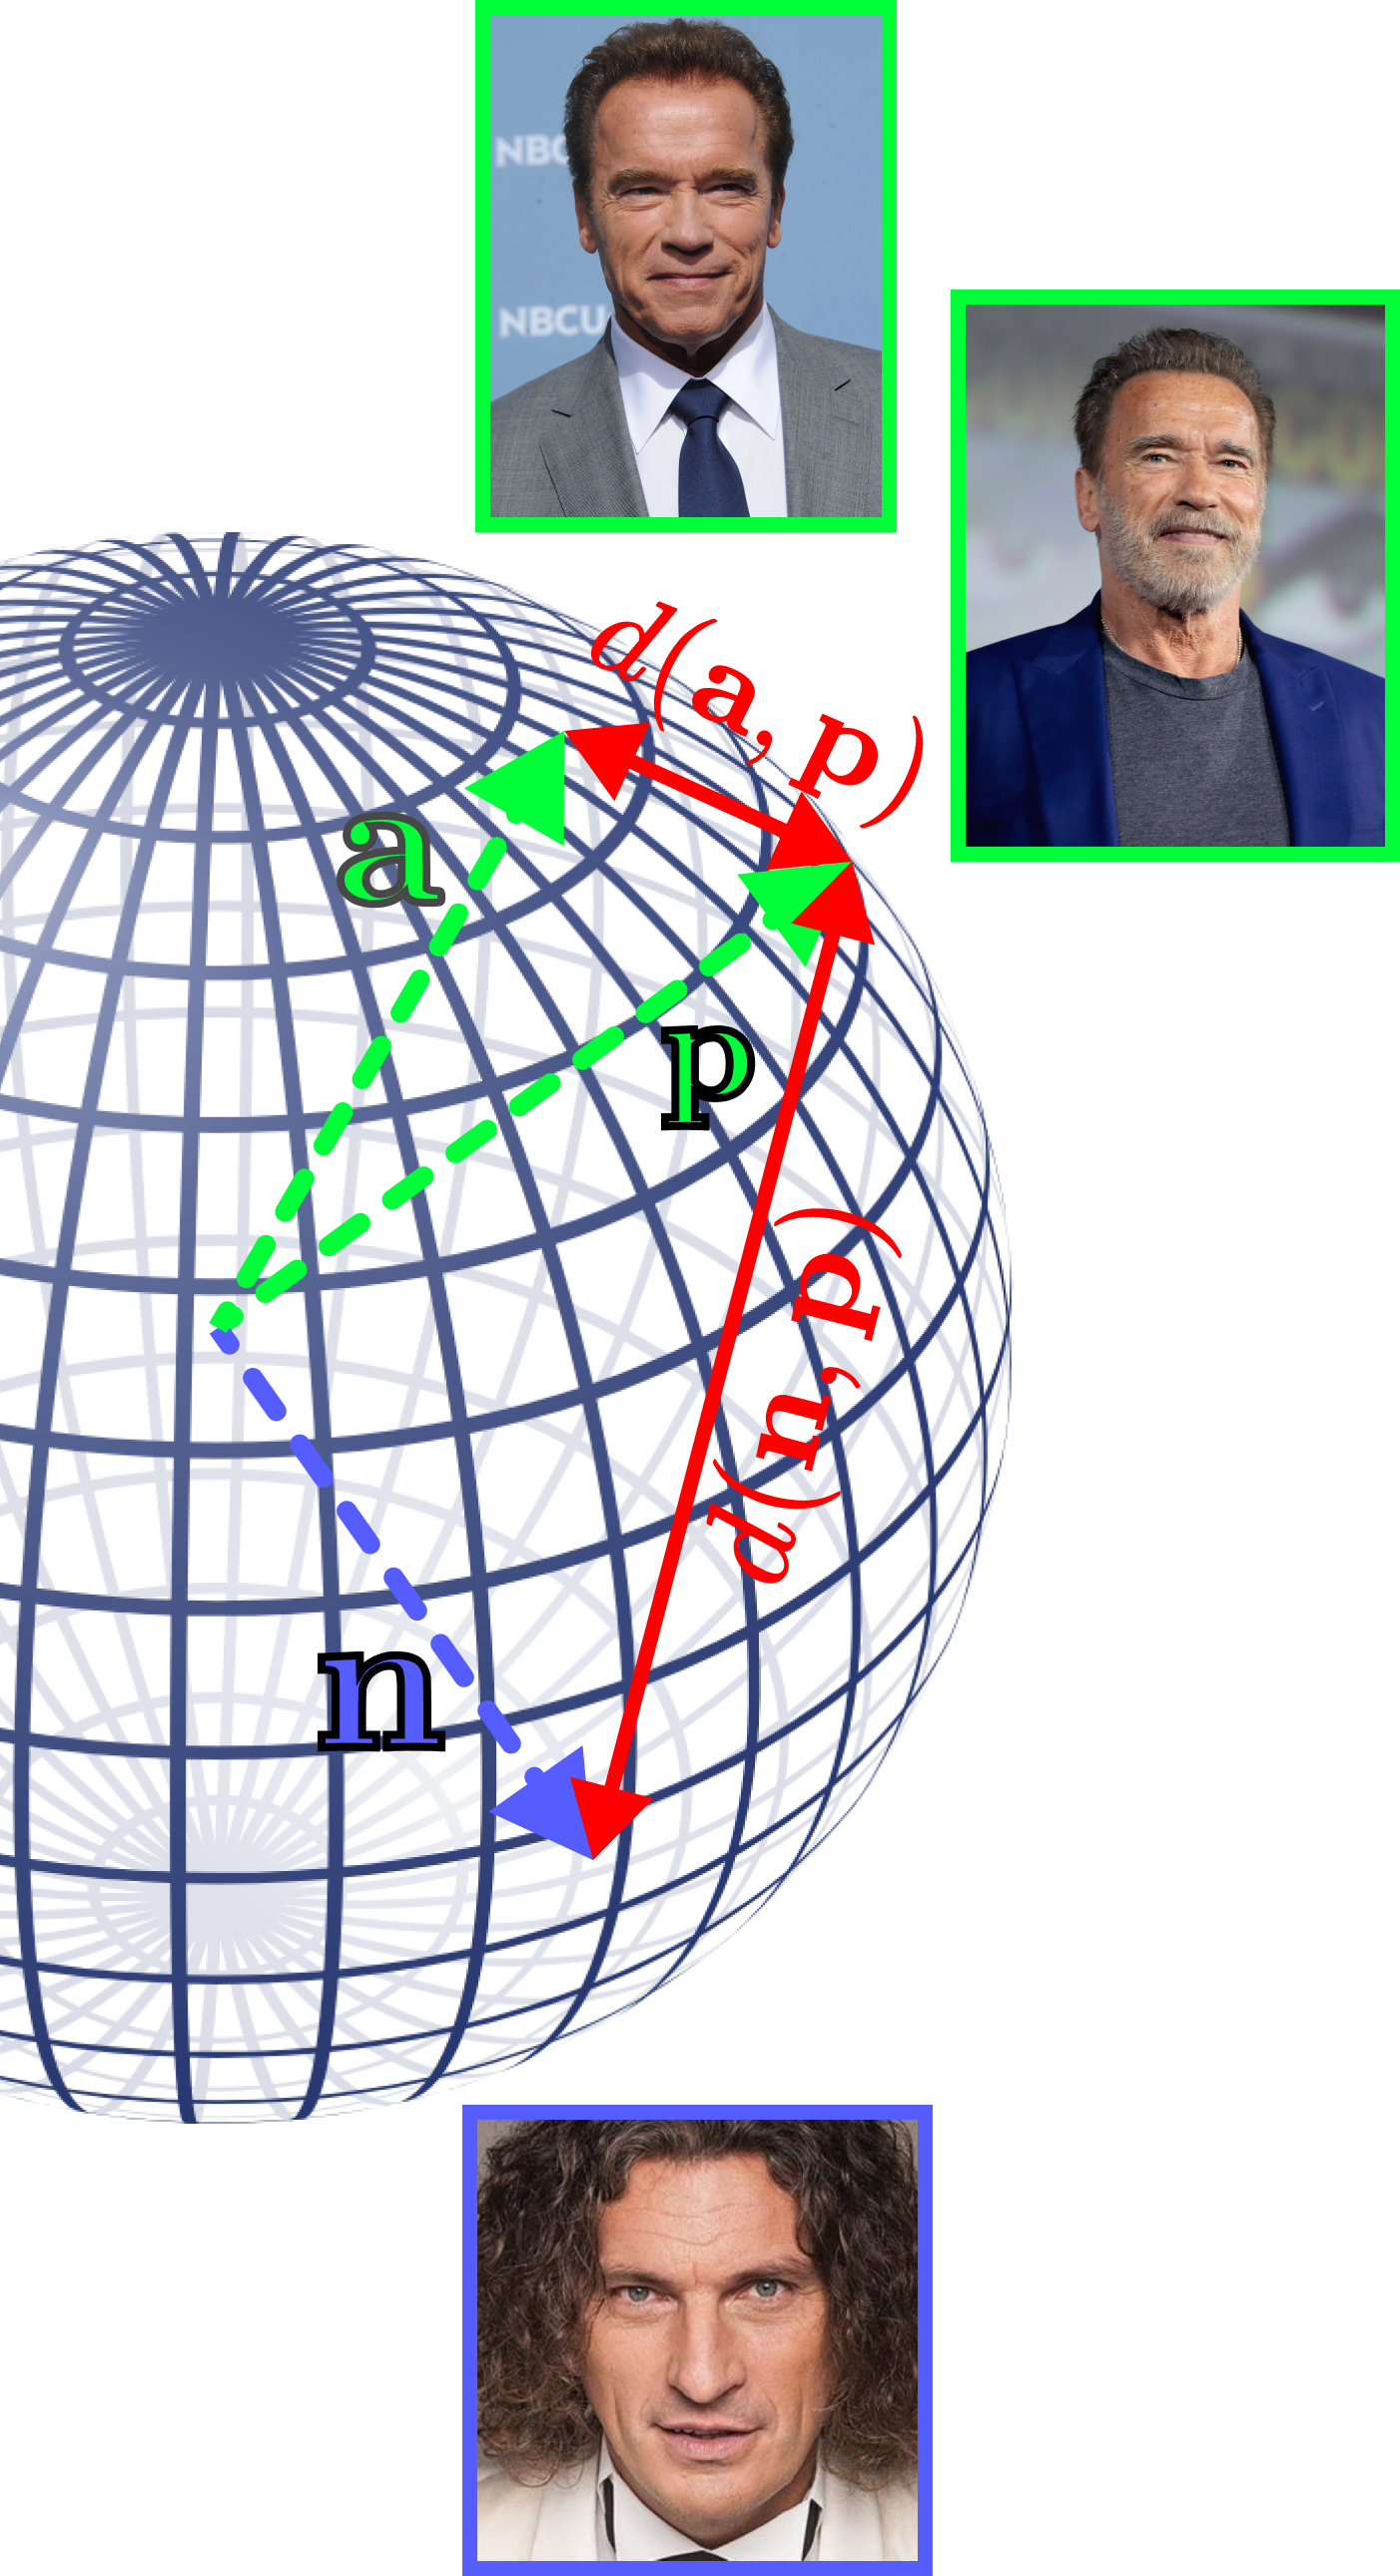
\includegraphics[width=0.6\textwidth]{images/hypersphere_dist.png}
            \caption{Метрика різниці людей -- відстань між векторами фіч}
        \end{figure}
        \end{column}

        \begin{column}{0.5\textwidth}
            Введемо відстань між векторами фіч $d(\cdot,\star)$. Найбільш частий вибор -- Евклідова метрика. 
        
            \textbf{Умова на одну людину:}
            \begin{equation*}
                \boxed{d(\mathcal{F}(X),\mathcal{F}(Y)) \leq \tau},
            \end{equation*}
            де $\tau$ -- так званий ``поріг'' або threshold.
        \end{column}
    \end{columns}
    \end{frame}

    \begin{frame}{Як реалізувати? Псевдокод}
        \textbf{Реєстрація:}

        \begin{enumerate}
            \item Прочитати зображення людини $X$ зі сканеру.
            \item Додати до бази данних $\mathcal{F}(X)$.
        \end{enumerate}

        \textbf{Автентифікація:}
        \begin{enumerate}
            \item Прочитати зображення людини $Y$ зі сканеру.
            \item Знайти вектор $y = \mathcal{F}(Y) = (y_1,\dots,y_{128})$.
            \item Для кожного вектору $z=(z_1,\dots,z_{128})$ з бази даних зробити наступну дію:
            \begin{enumerate}
                \item Якщо $\sum_{i=1}^{128}(y_i-z_i)^2 < \tau$ -- впустити людину.
                \item Якщо ні, то продовжити.
            \end{enumerate}
        \end{enumerate}

        \begin{block}{Резюме}
            Всі ми -- просто набір $128$ дійсних чисел на гіперсфері :(
        \end{block}
    \end{frame}

    \subsection{Тріплет мережа}
    \begin{frame}{Як навчати? Головна ідея}
        Візьмемо три фотографії:
        \begin{itemize}
            \item $A$ (anchor) -- зображення людини 1.
            \item $P$ (positive) -- інше зображення людини 1.
            \item $N$ (negative) -- зображення людини 2.
        \end{itemize}
        Головне, що ми хочемо:
        \begin{equation*}
            d(A,P) < d(A,N)
        \end{equation*}
        Або, більш строга умова умова:
        \begin{equation*}
            d(A,P) < d(A,N) - \gamma
        \end{equation*}
        

        \begin{figure}
        \centering
            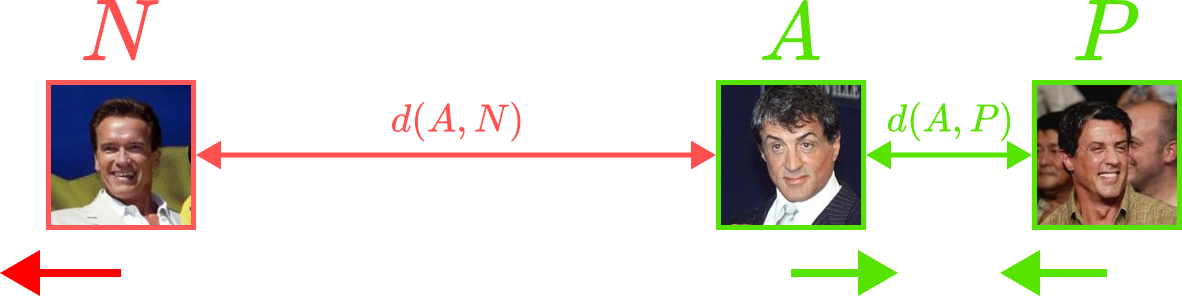
\includegraphics[width=0.8\textwidth]{images/triplet_dist.png}
        \end{figure}
    \end{frame}

    \begin{frame}{Як навчати? Робимо метрику!}
        Як з цієї ідеї зробити конкретну метрику (втрату)? 
        
        Використовується наступна функція:
        \begin{equation*}
            \ell(A,P,N) = \max\left\{d(A,P)-d(A,N)+\gamma,0\right\}
        \end{equation*}

        \begin{figure}
        \centering
            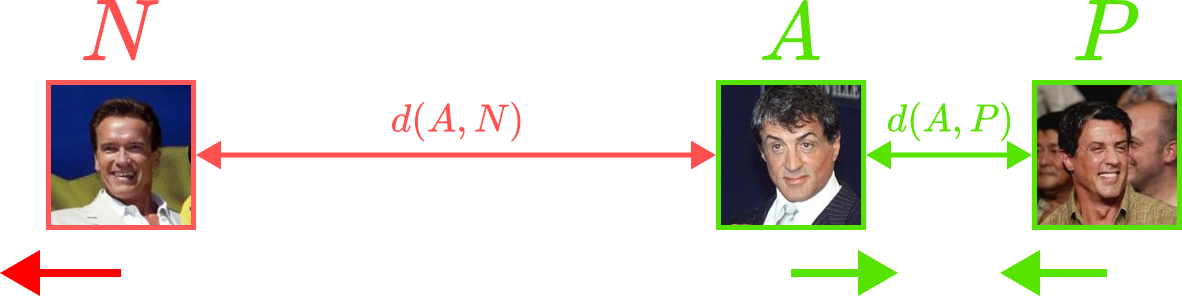
\includegraphics[width=0.8\textwidth]{images/triplet_dist.png}
            \caption{Після застосування градієнту, ми хочемо віддалити $(A,N)$ і наблизити $(A,P)$.}
        \end{figure}
    \end{frame}

    \begin{frame}{Як навчати? Triplet Network}
        Як побудувати нейронну мережу? Triplet Network!
        
        \begin{figure}
        \centering
            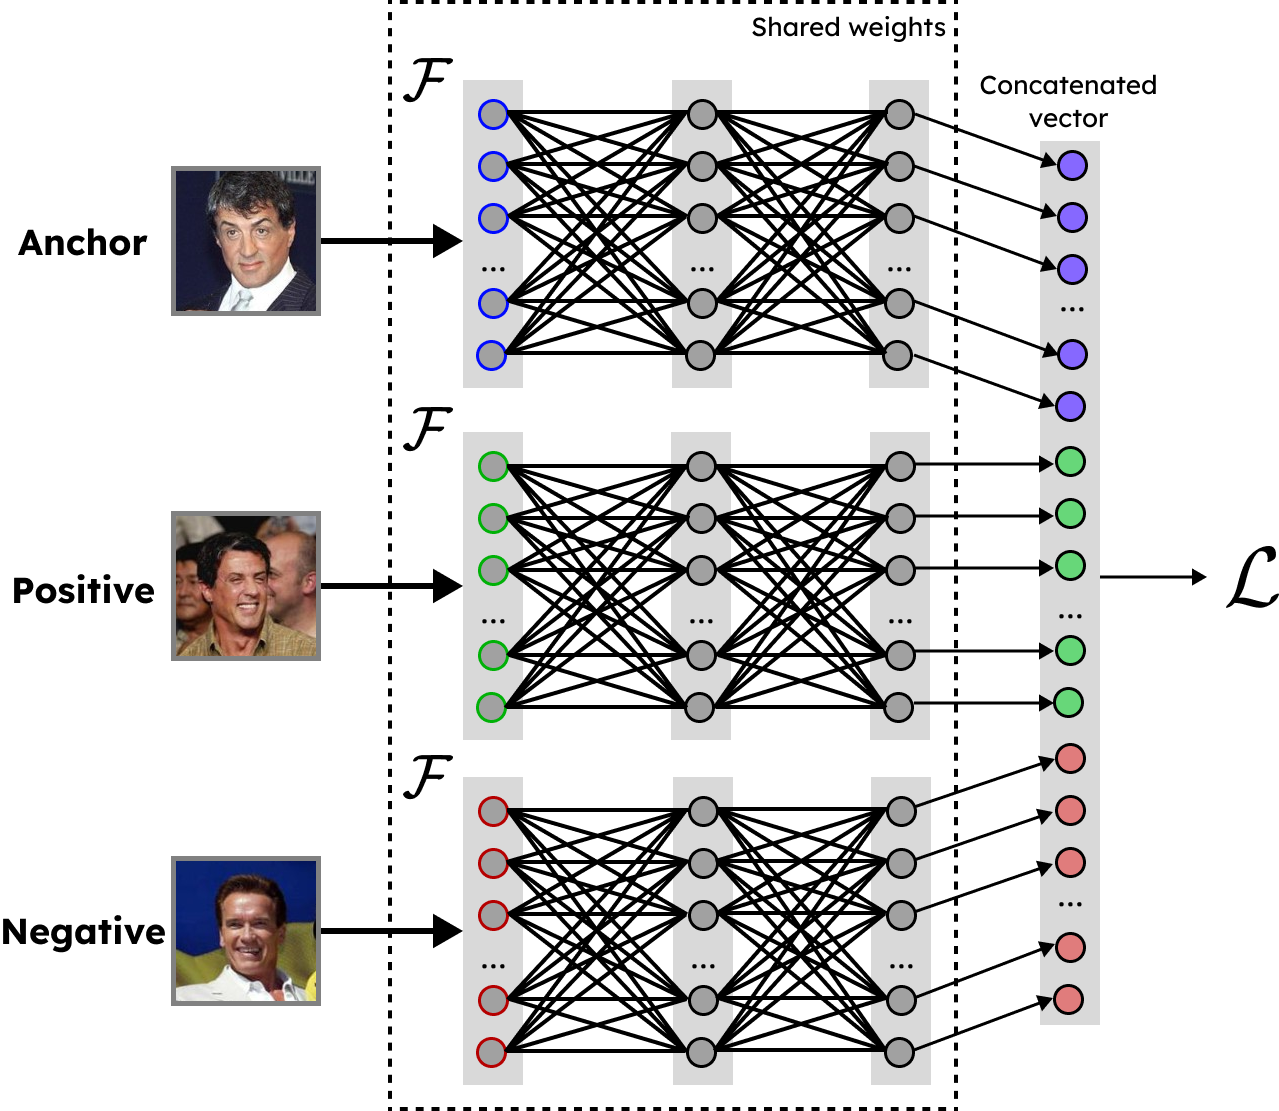
\includegraphics[width=0.6\textwidth]{images/triplet_network.png}
            \caption{Triplet Network архітектура.}
        \end{figure}
    \end{frame}

    \section{Ідентифікуємий, але не впізнаємий}

    \begin{frame}{Безпека векторів фіч}
        \begin{itemize}
            \item Зберігати зображення в базі данних небезпечно.
            \item Чи безпечно зберігати вектори фіч? Ні.
            \item Чи можна створити криптографічний примітив? Дуже активна робота саме в цьому напрямку!
        \end{itemize}

        \begin{figure}
        \centering
            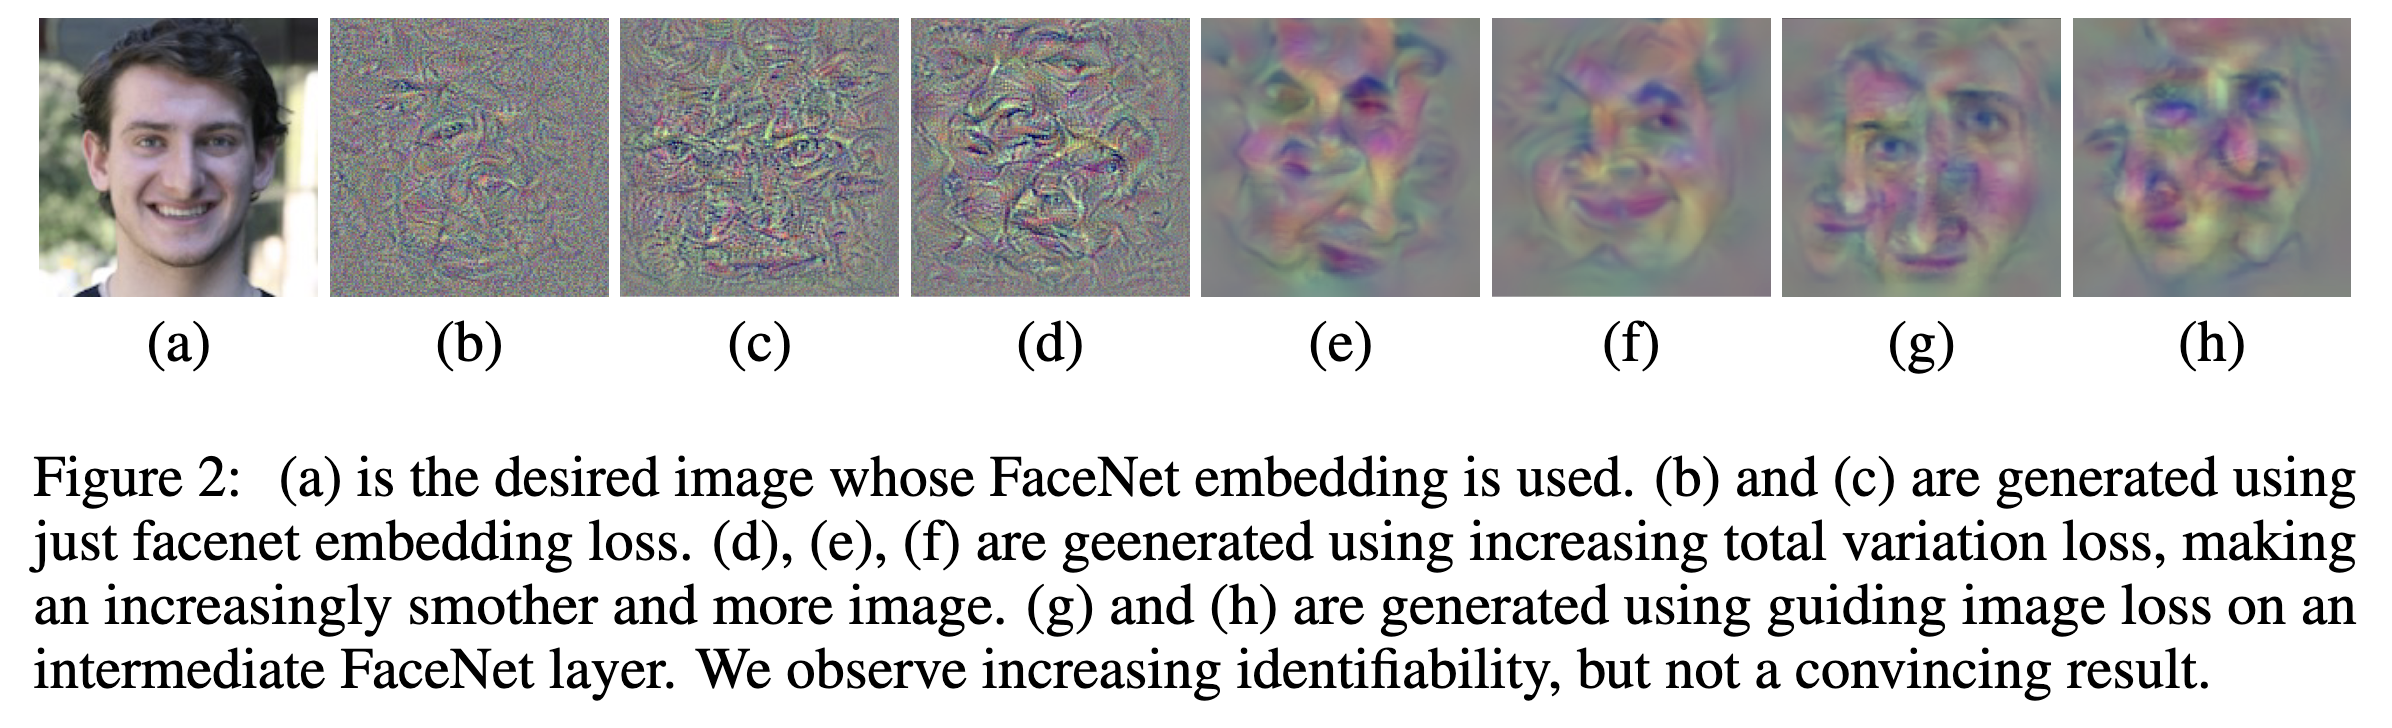
\includegraphics[width=\textwidth]{images/inverting_facenet.png}
            \caption{Знаходження обличчя з векторів фіч. Взято з Edward Vendrow et al. 2018. Inverting Facial Embeddings with GANs}
        \end{figure}
    \end{frame}

    \begin{frame}{Безпека векторів фіч}
        \begin{figure}
        \centering
            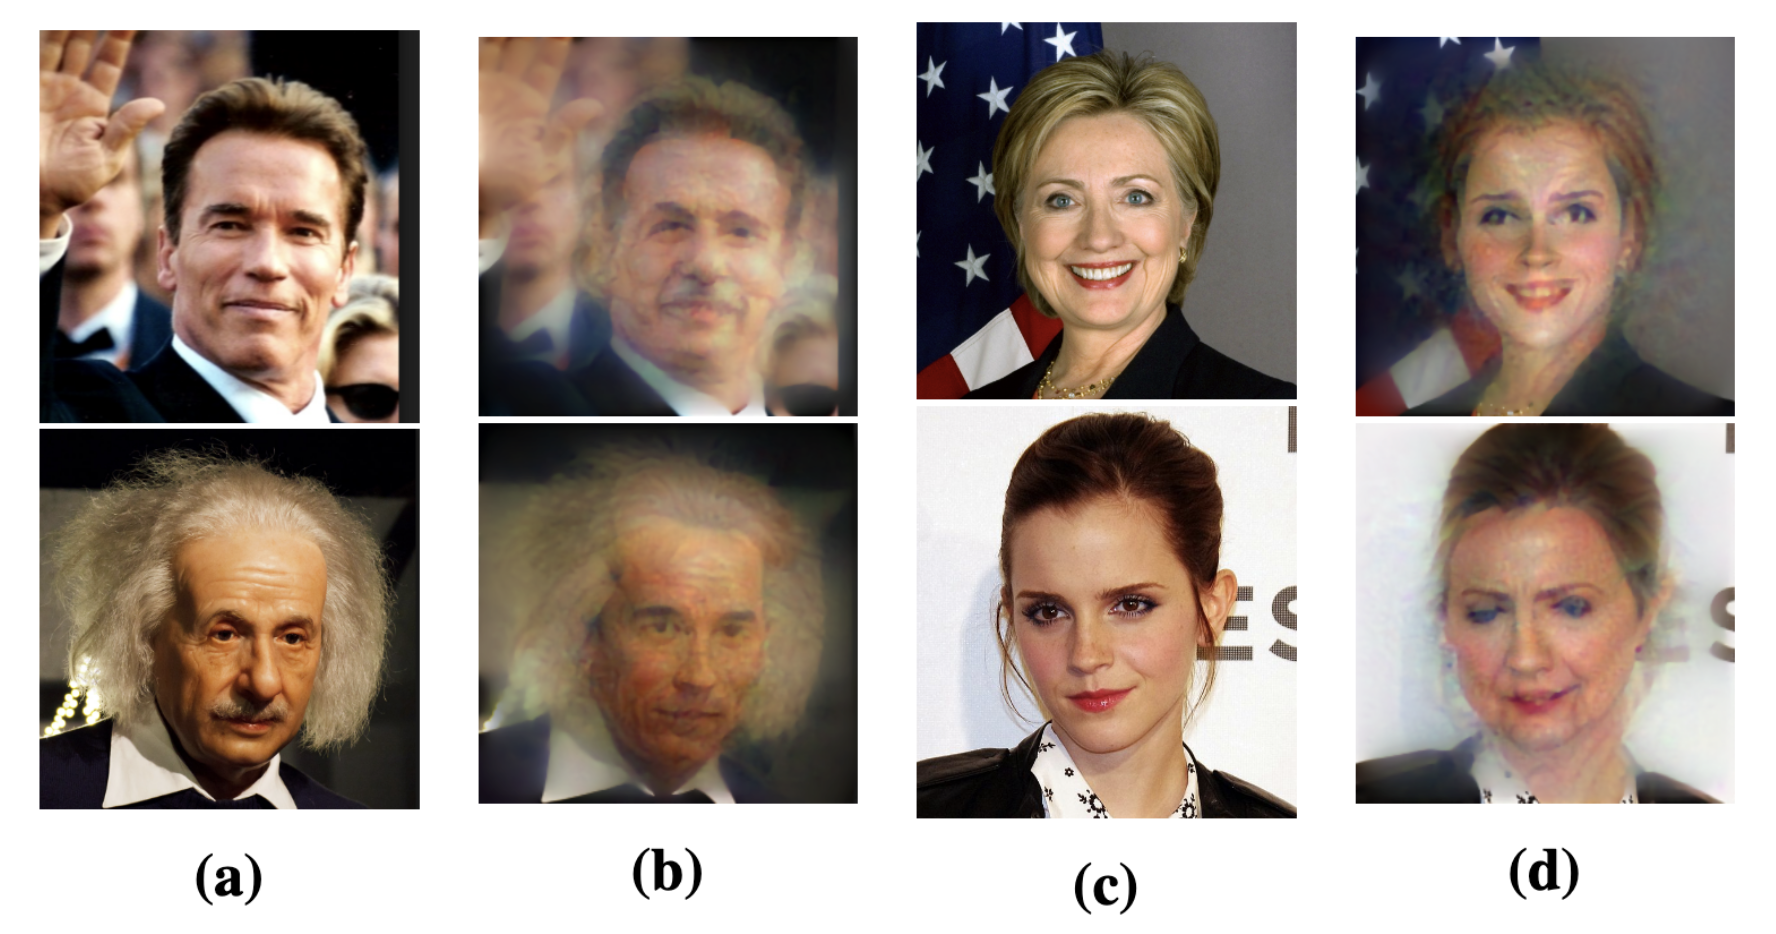
\includegraphics[width=0.8\textwidth]{images/invert_emb.png}
            \caption{Обернення FaceNet, використовуючи базове зображення. Andrey Zhmoginov et al. ``Inverting face embeddings with convolutional neural networks''}
        \end{figure}
    \end{frame}

    \begin{frame}{Відміняєма біометрія}
        \begin{figure}
        \centering
            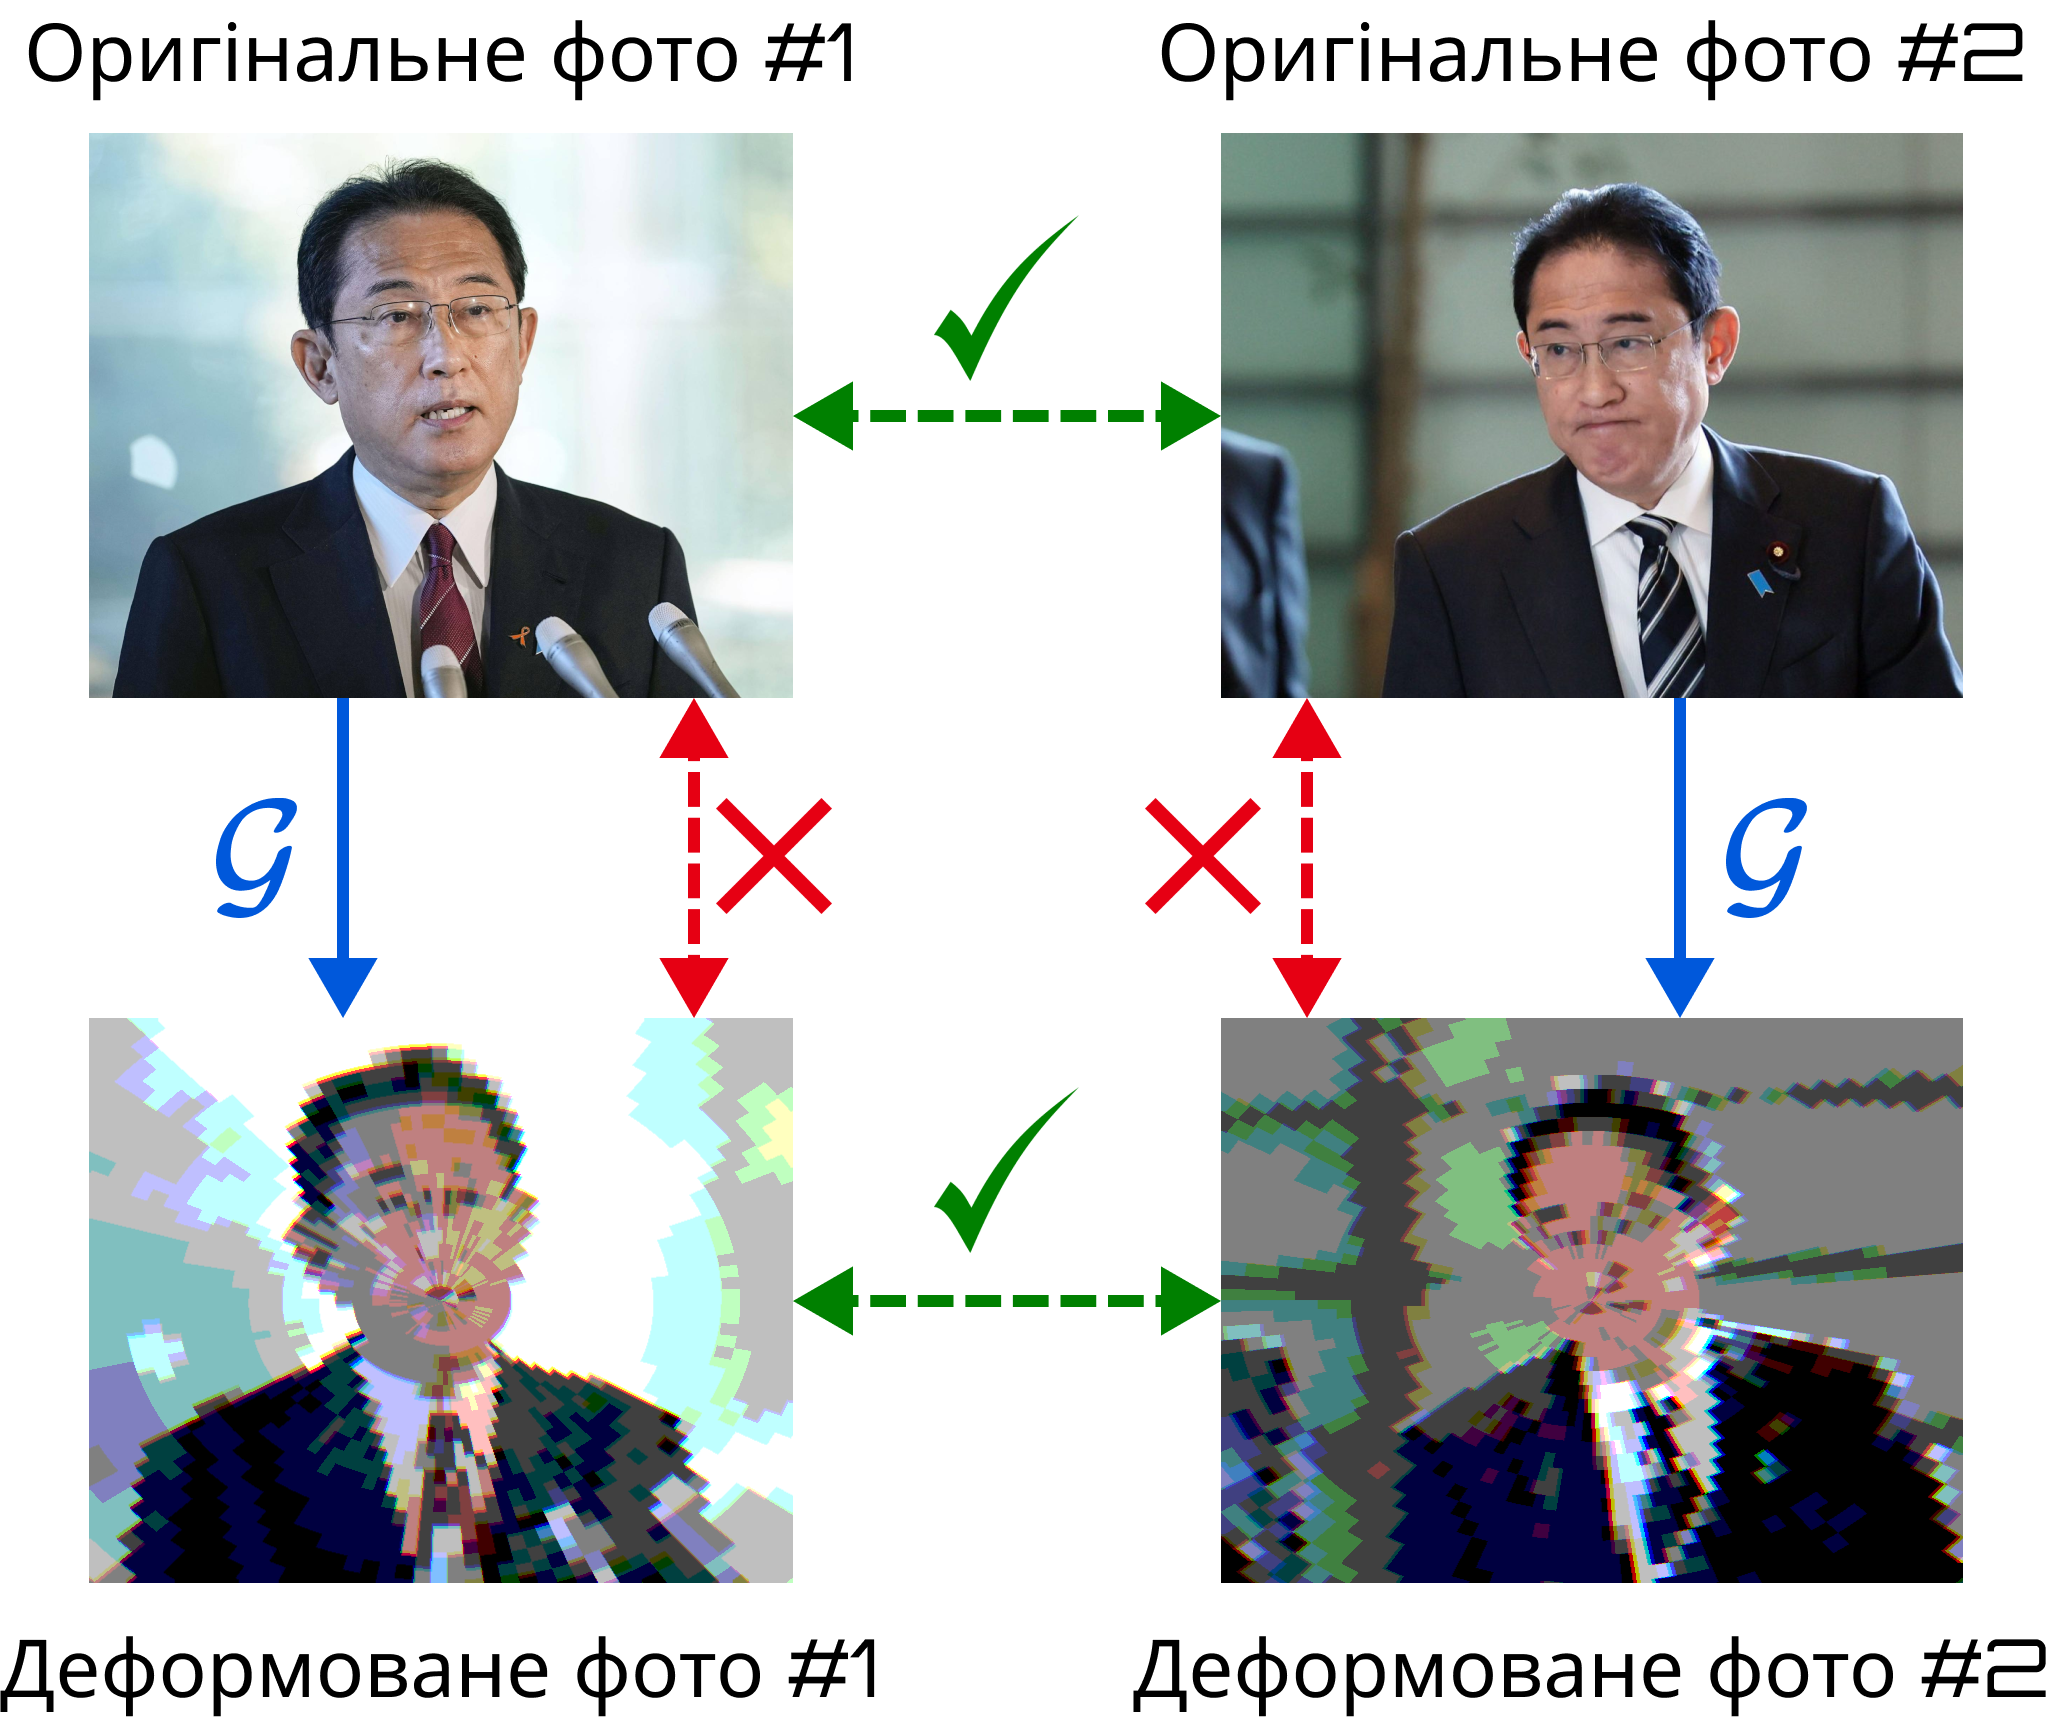
\includegraphics[width=0.65\textwidth]{images/cancelable_biometrics.png}
            \caption{Система відміняємої біометрії. Функція $\mathcal{G}$, переводить зображення у простір деформованих фото, в якому можна порівнювати зображення.}
        \end{figure}
    \end{frame}

    \begin{frame}{Шифрування}
        \begin{figure}
        \centering
            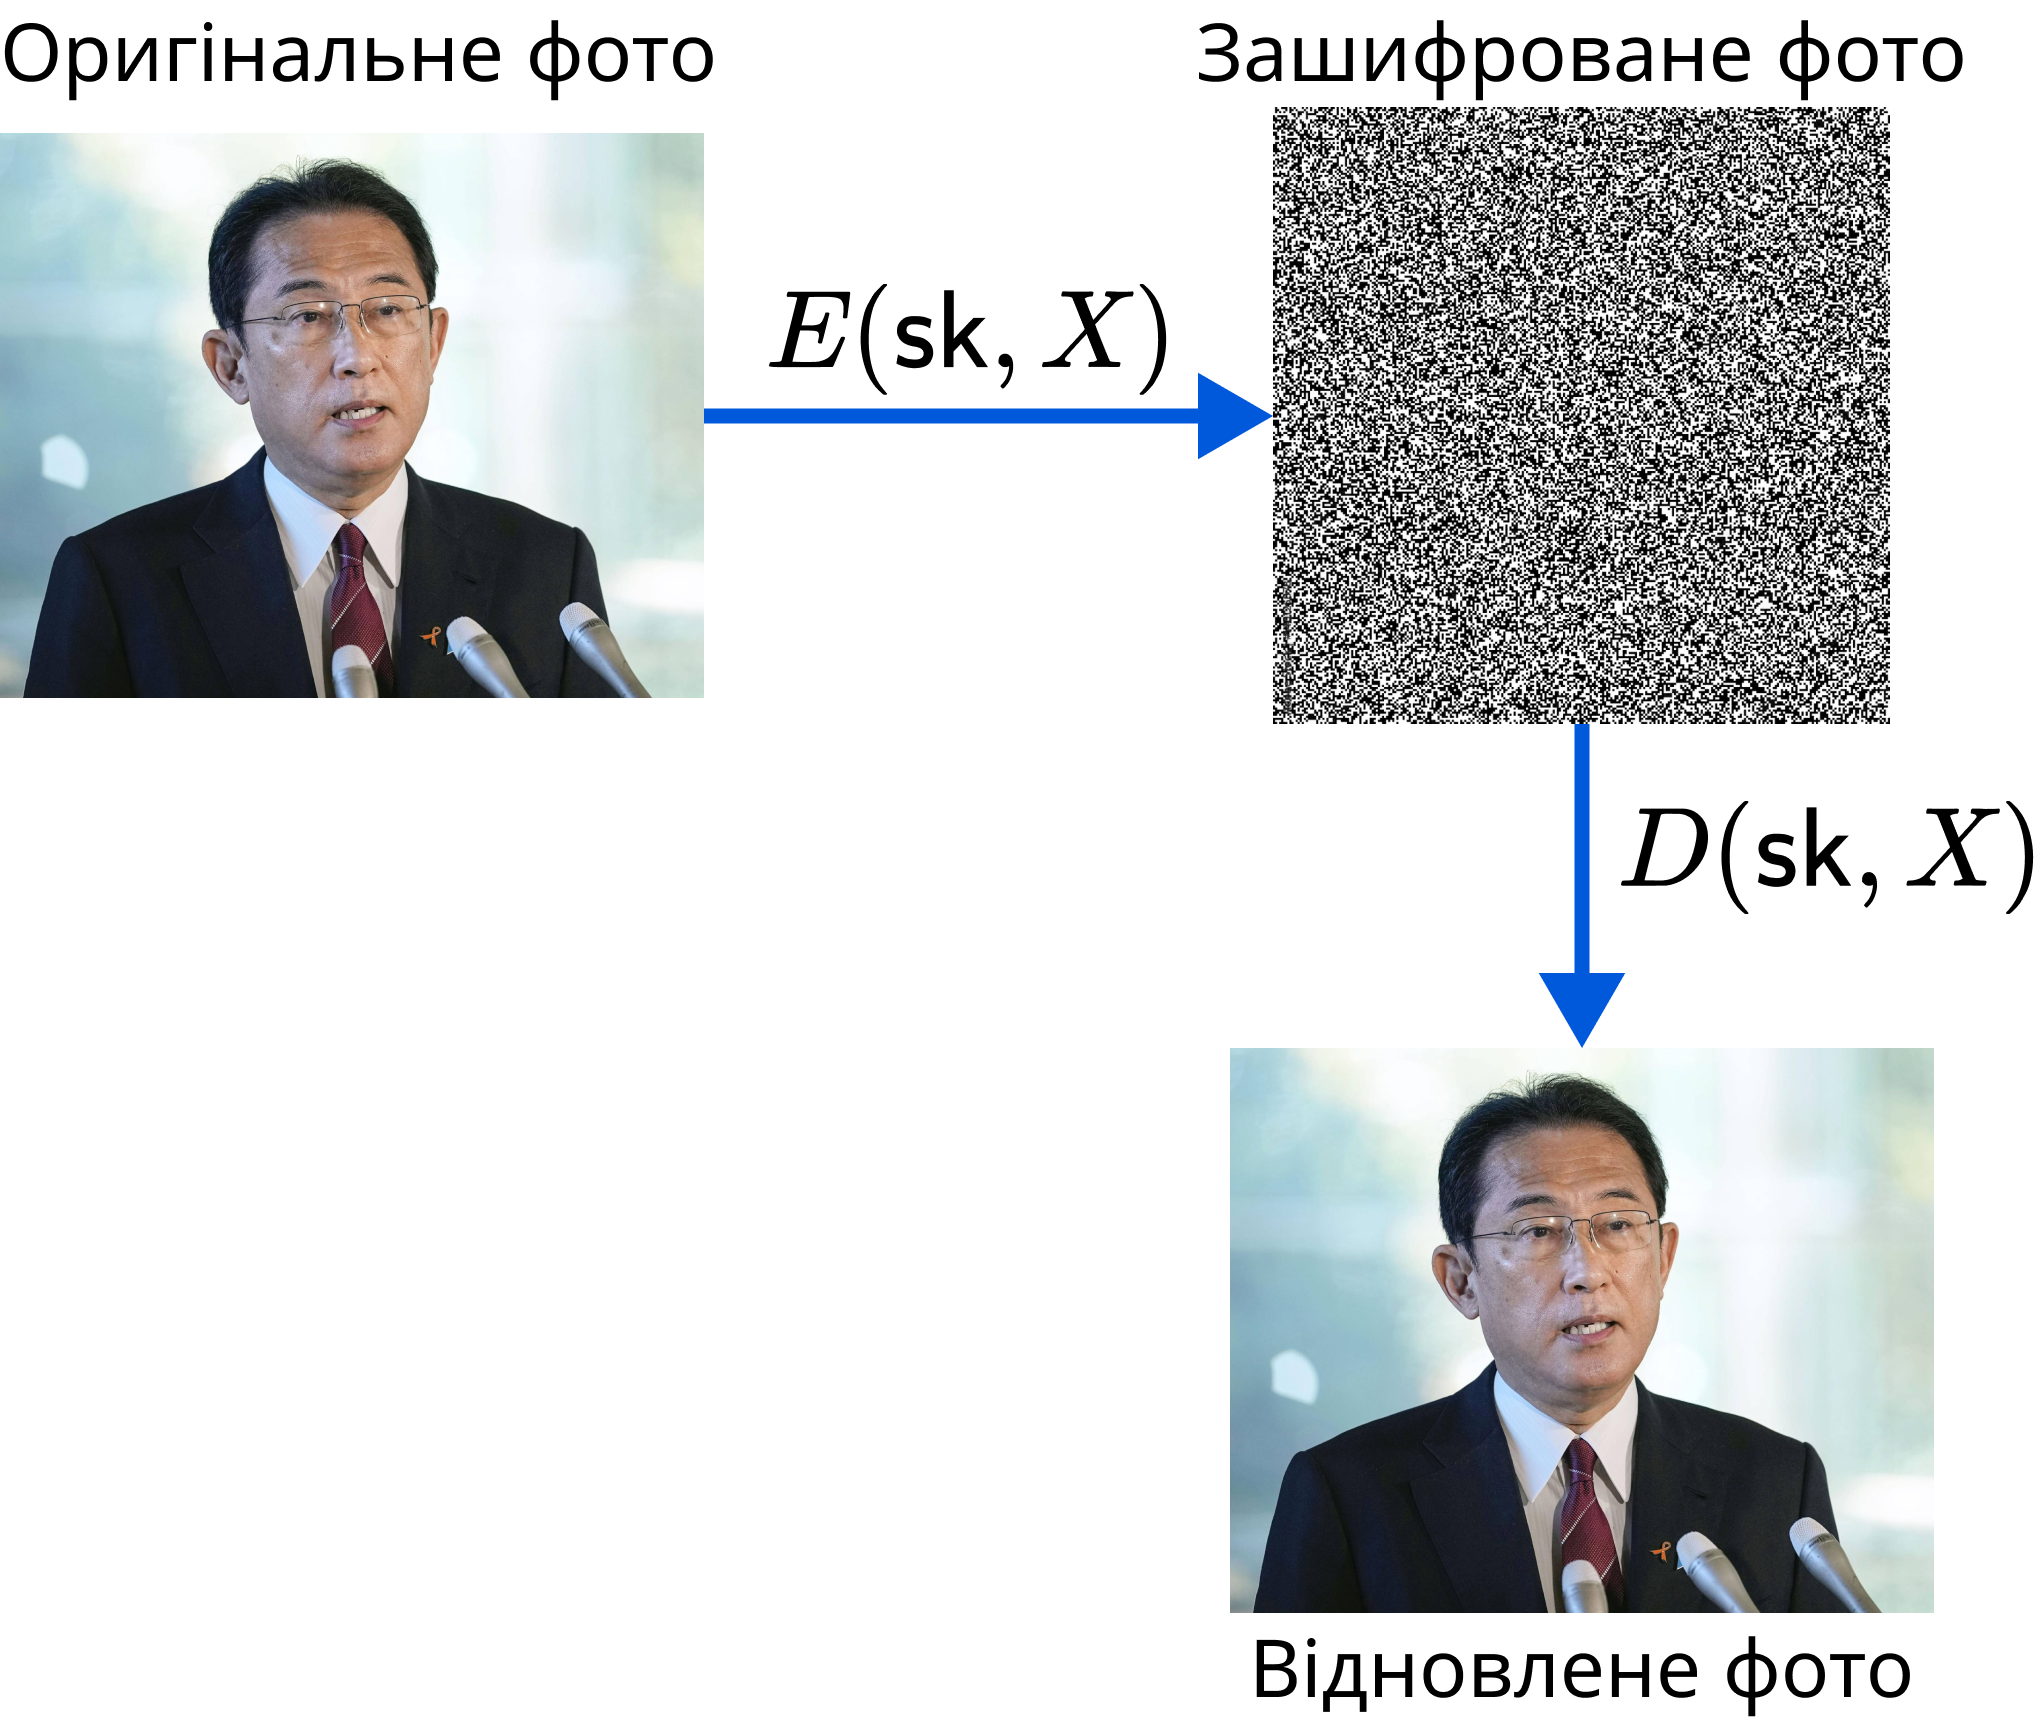
\includegraphics[width=0.6\textwidth]{images/cipher.png}
            \caption{Система (симетричного) шифрування. Маємо функцію шифрування $E(\mathsf{sk},X)$ та дешифрування $D(\mathsf{sk},C)$ з умовою коректності $D(\mathsf{sk},E(\mathsf{sk},X))=X$.}
        \end{figure}
    \end{frame}

    \begin{frame}{Проблема}
        Нехай ми подали зображення $X$ на вхід і хочемо порівняти з зашифрованним шаблоном $T$ в базі данних.
        \begin{itemize}
            \item \textit{Відміняєма біометрія} спочатку трансформує зображення $\mathcal{G}(X)$, а потім порівнює з шаблоном: $d(\mathcal{G}(X),T) \stackrel{?}{\leq} \tau$.
            \item \textit{Шифрування} спочатку декодує зображення $D(\mathsf{sk},T)$, а потім порівнює з вхідним: $d(D(\mathsf{sk},T),X) \stackrel{?}{\leq} \tau$.
        \end{itemize}
        В будь-якому випадку, маємо дві дії: предобробка зображення, а потім порівняння. Чи можна це звести у лише одне порівняння: $d^*(X,T) \stackrel{?}{\leq} \tau$?
    \end{frame}

    \begin{frame}{Наше рішення}
        \begin{columns}
        % Description
        \begin{column}{0.5\textwidth}
        \begin{figure}
        \centering
            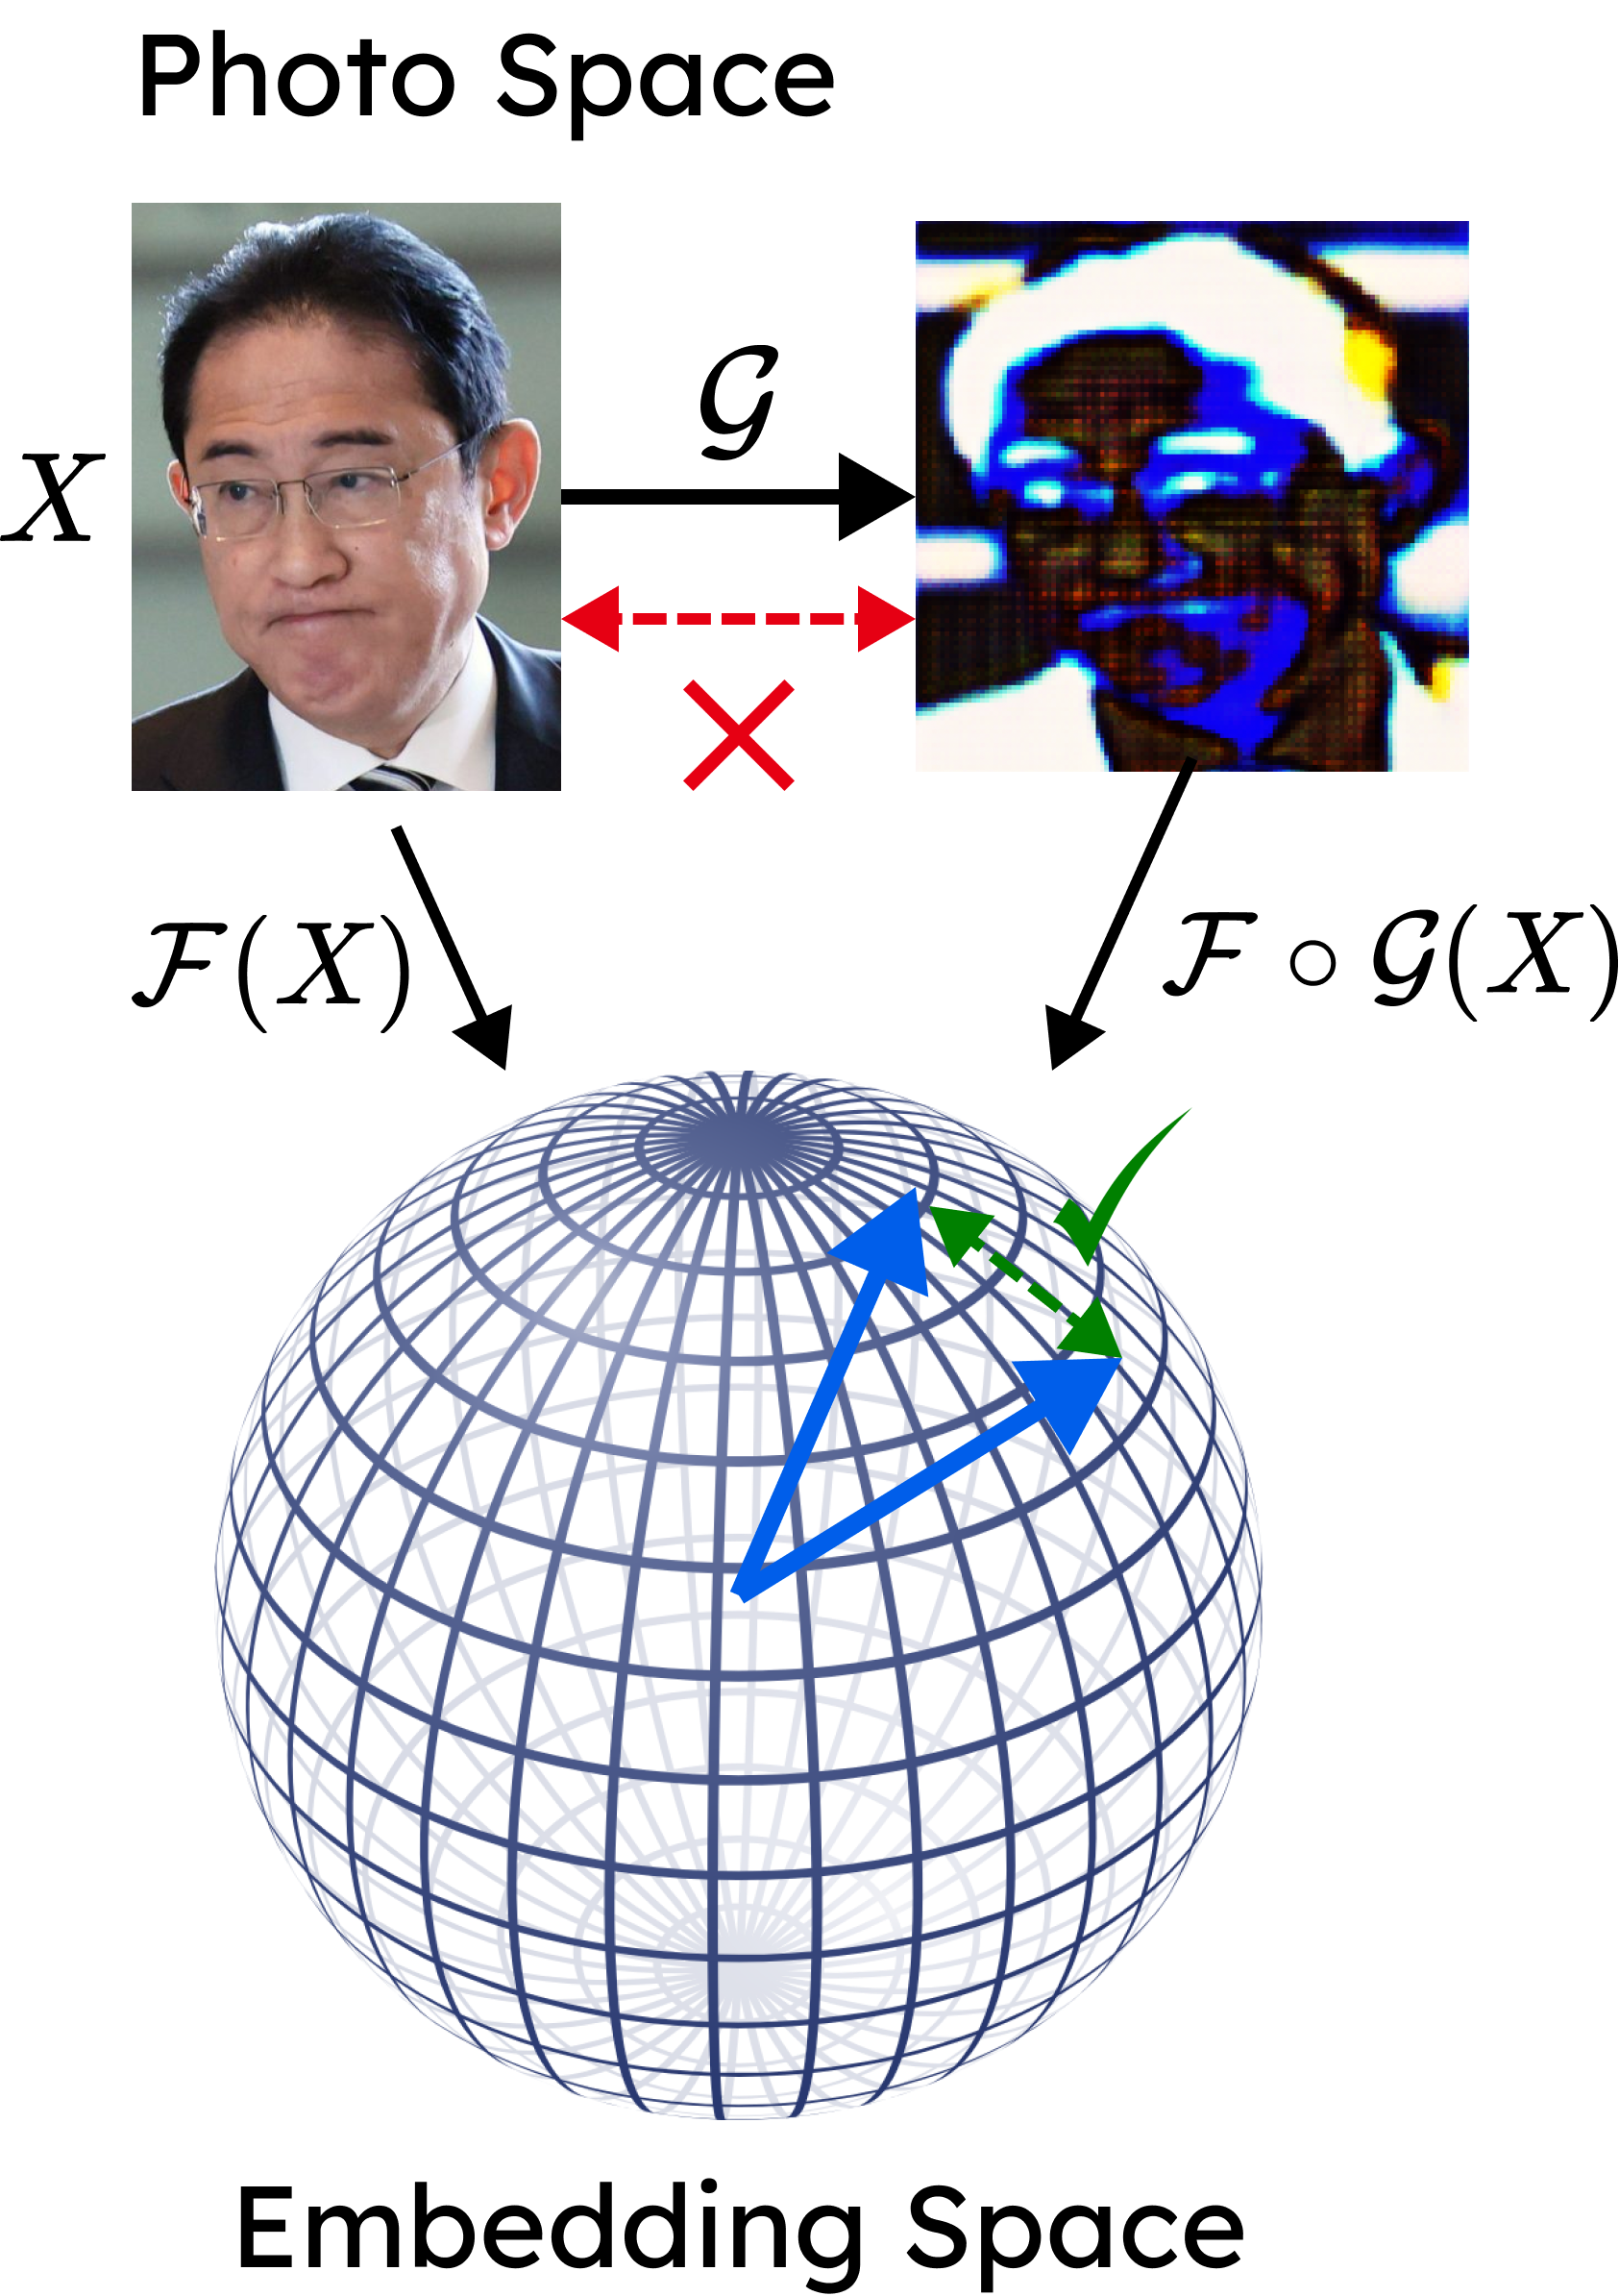
\includegraphics[width=0.8\textwidth]{images/our_approach.png}
            \caption{Ілюстрація нашого методу.}
        \end{figure}
        \end{column}

        \begin{column}{0.5\textwidth}
            Система захисту складається з пари $(\mathcal{G},\mathcal{F})$, де:
            \begin{itemize}
                \item $\mathcal{G}$ -- генератор деформованих фото;
                \item $\mathcal{F}$ -- embedding нейронна мережа.
            \end{itemize}
            \textbf{Головні властивості:}
            \begin{itemize}
                \item $\mathcal{F}(X) \approx \mathcal{F}(\mathcal{G}(X))$. 
                \item $\mathcal{G}^{-1}$ ``складно'' обрахувати.
            \end{itemize}
        \end{column}
    \end{columns}
    \end{frame}

    \begin{frame}{Оптимізаційна задача -- візуалізація}
        \begin{figure}
        \centering
            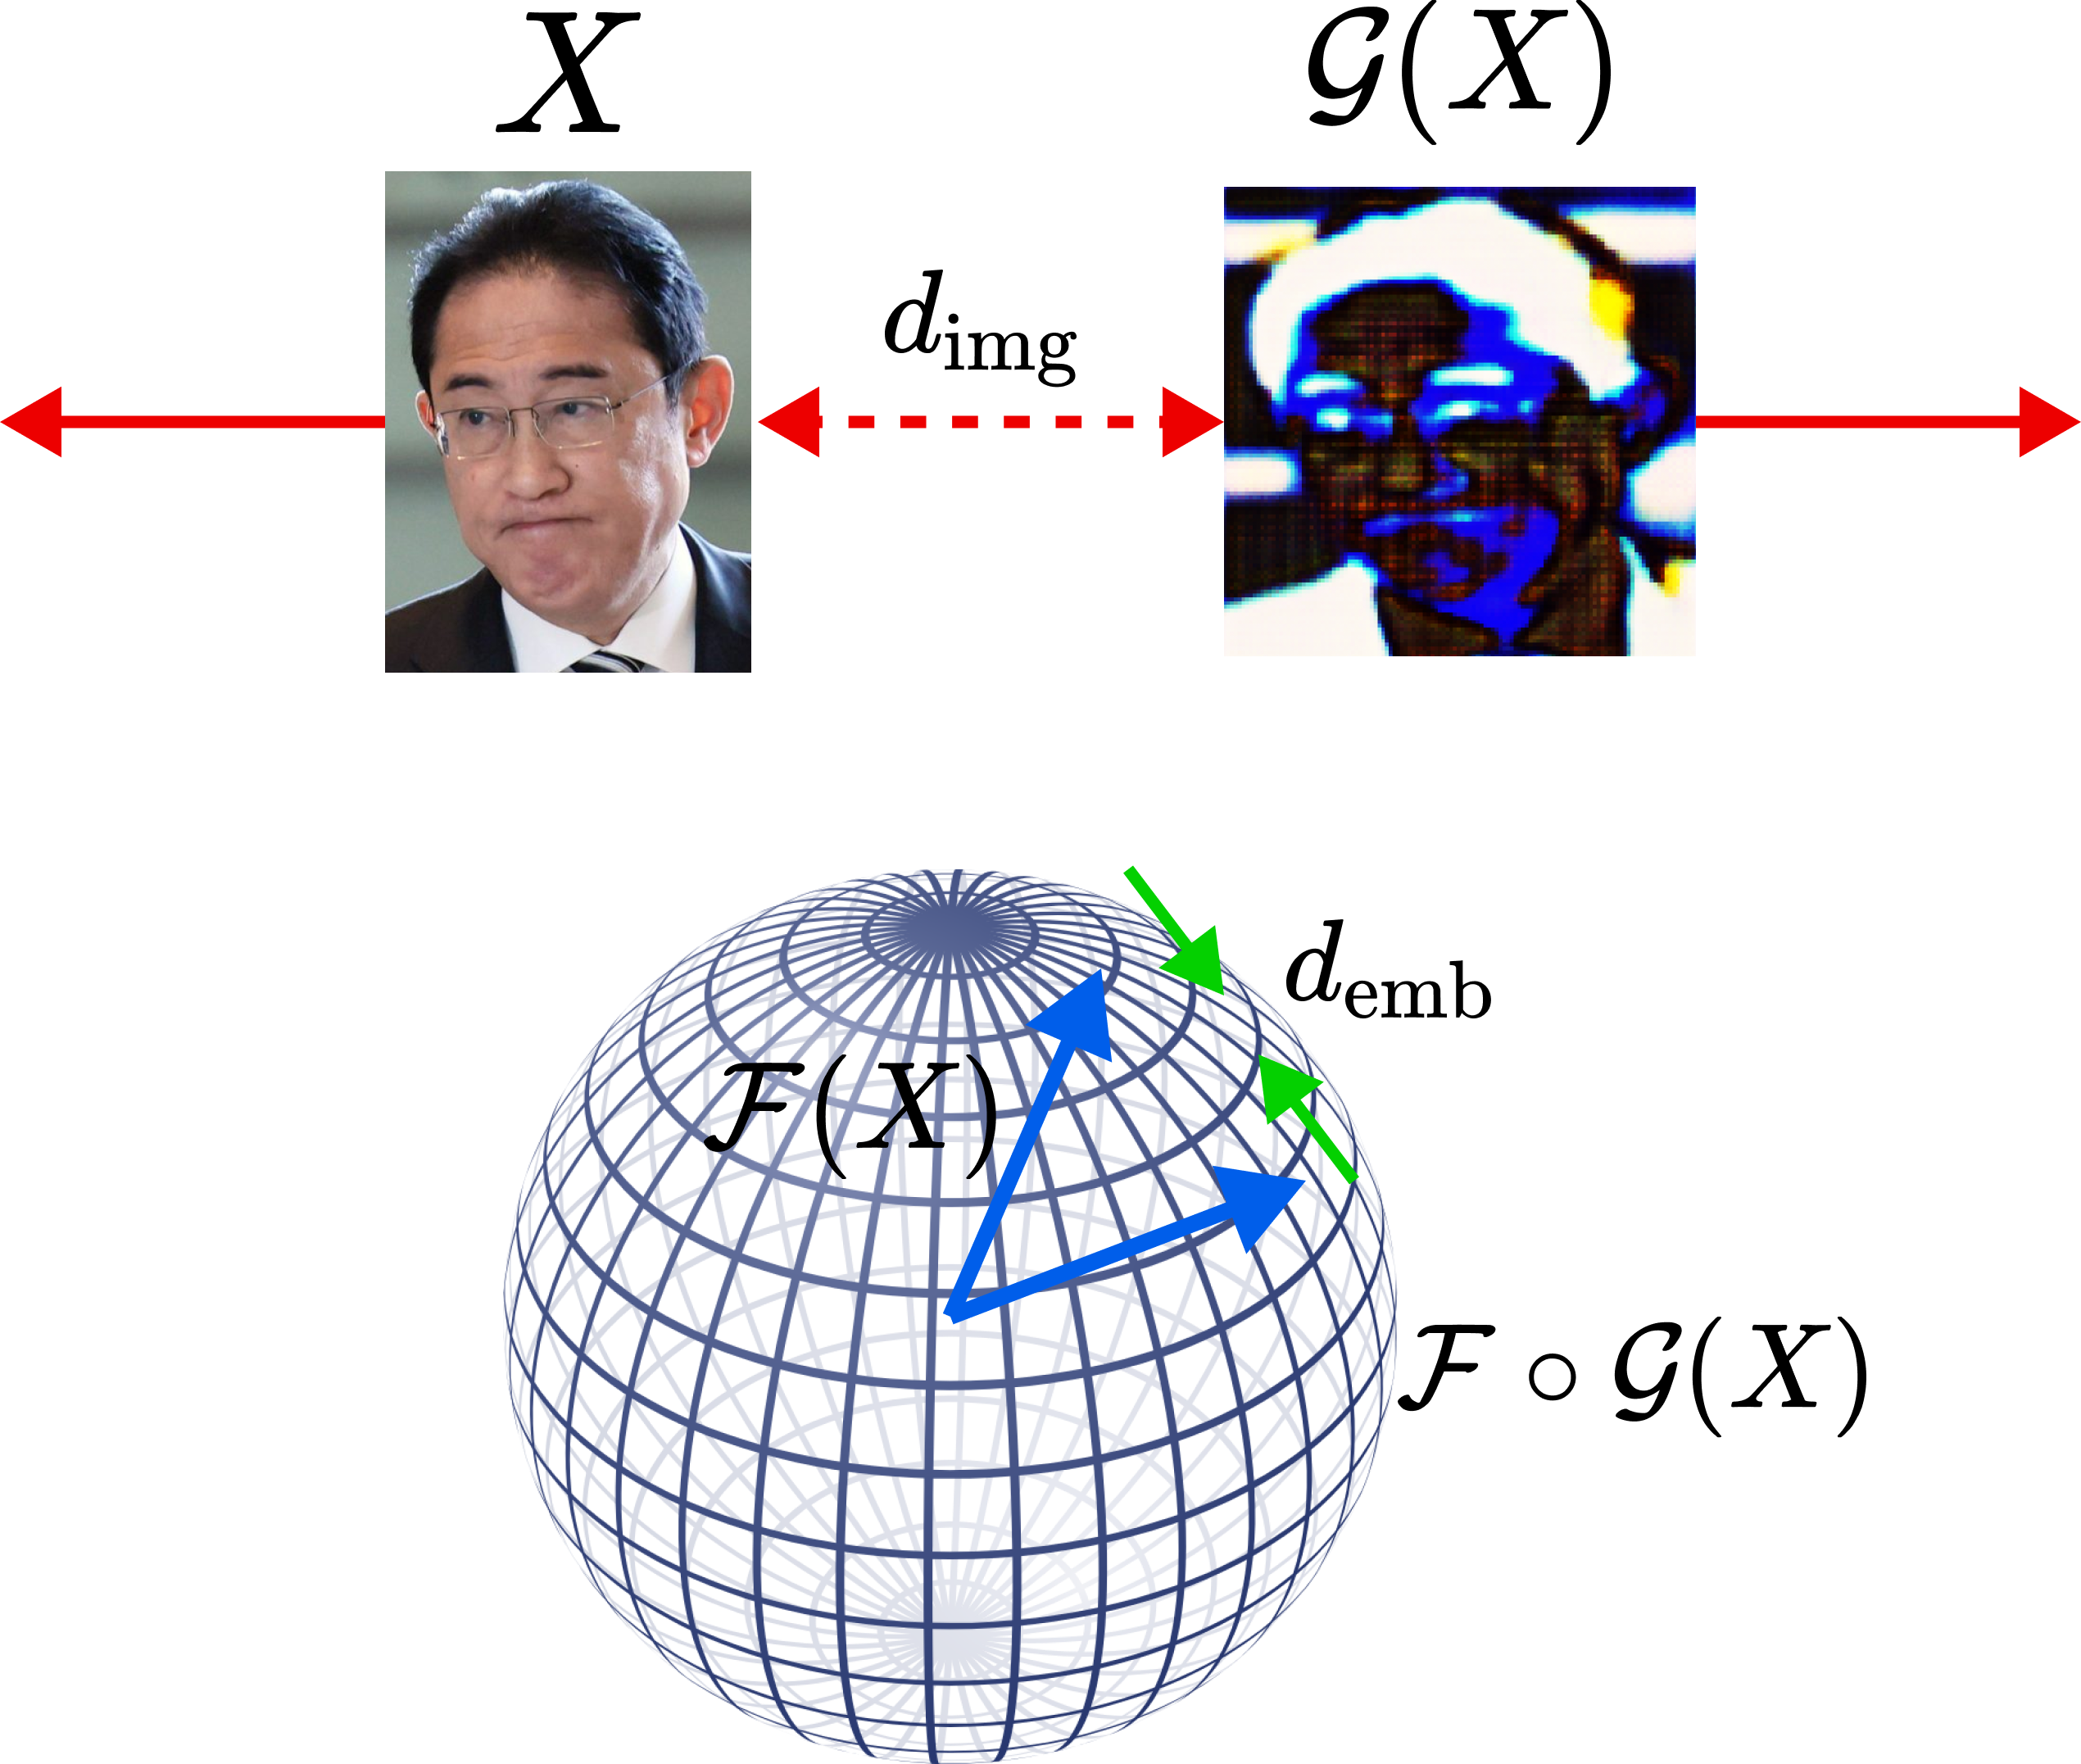
\includegraphics[width=0.6\textwidth]{images/idea_vis.png}
            \caption{Візуалізація цілі задачі.}
        \end{figure}
    \end{frame}

    \begin{frame}{Trainer Network}
        \begin{figure}
        \centering
            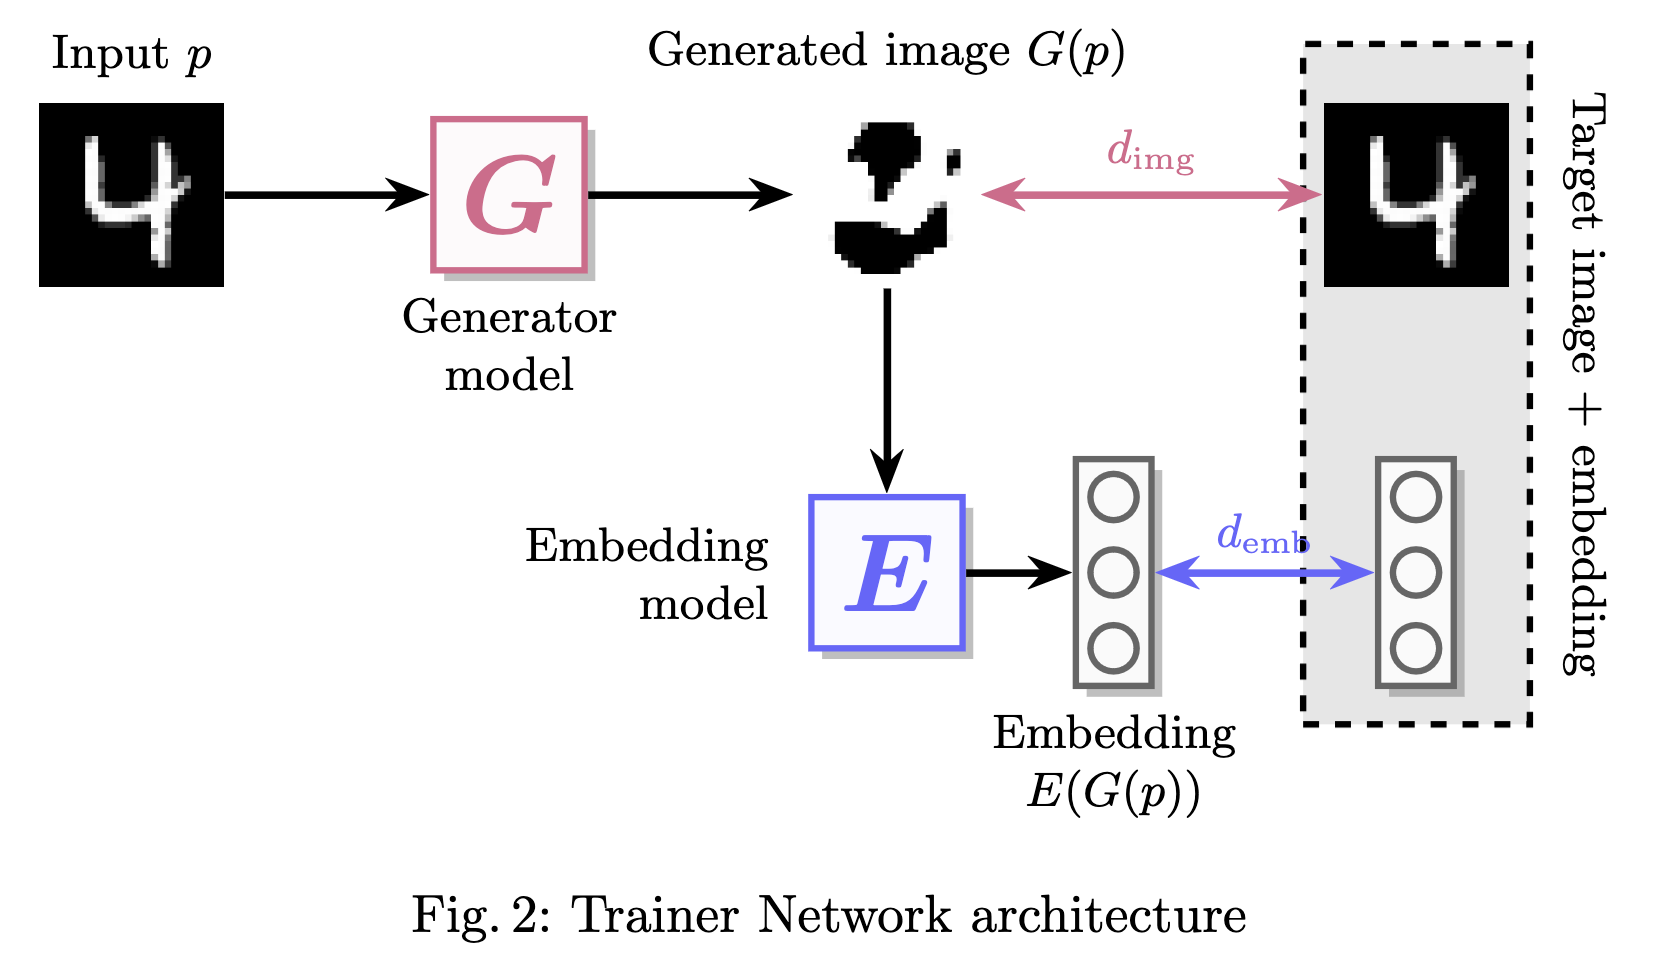
\includegraphics[width=\textwidth]{images/trainer.png}
            \caption{Ілюстрація Trainer Network архітектури з нашої роботи.}
        \end{figure}
    \end{frame}

    \begin{frame}{U-Net}
        \begin{figure}
        \centering
            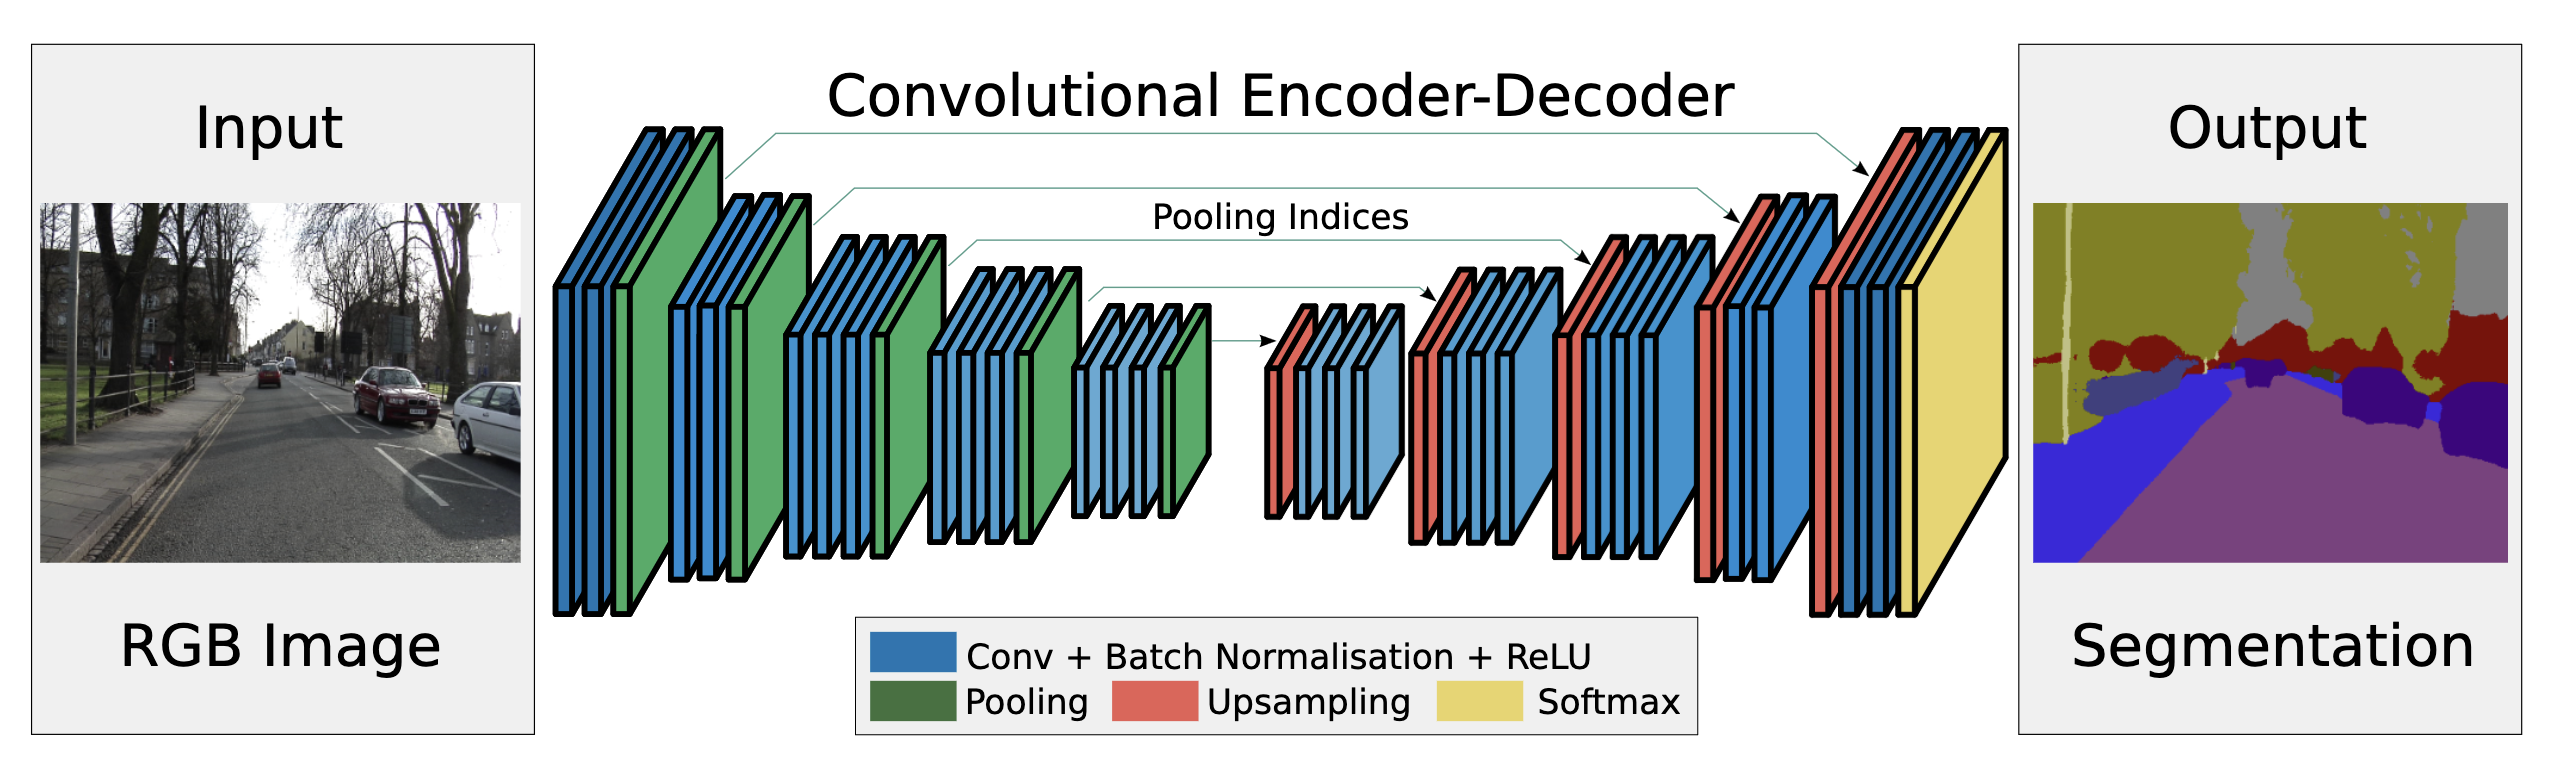
\includegraphics[width=\textwidth]{images/unet.png}
            \caption{U-Net архітектура (Encoder $\to$ Decoder). Спочатку зображення стискається, а потім розтискається.
            \scriptsize Ілюстрація взята з K. Murphy ``Probabilistic Machine Learning: An introduction''. MIT Press. 2022}
        \end{figure}
    \end{frame}

    \begin{frame}{Приклади зображень. MNIST}
        \begin{figure}
        \centering
            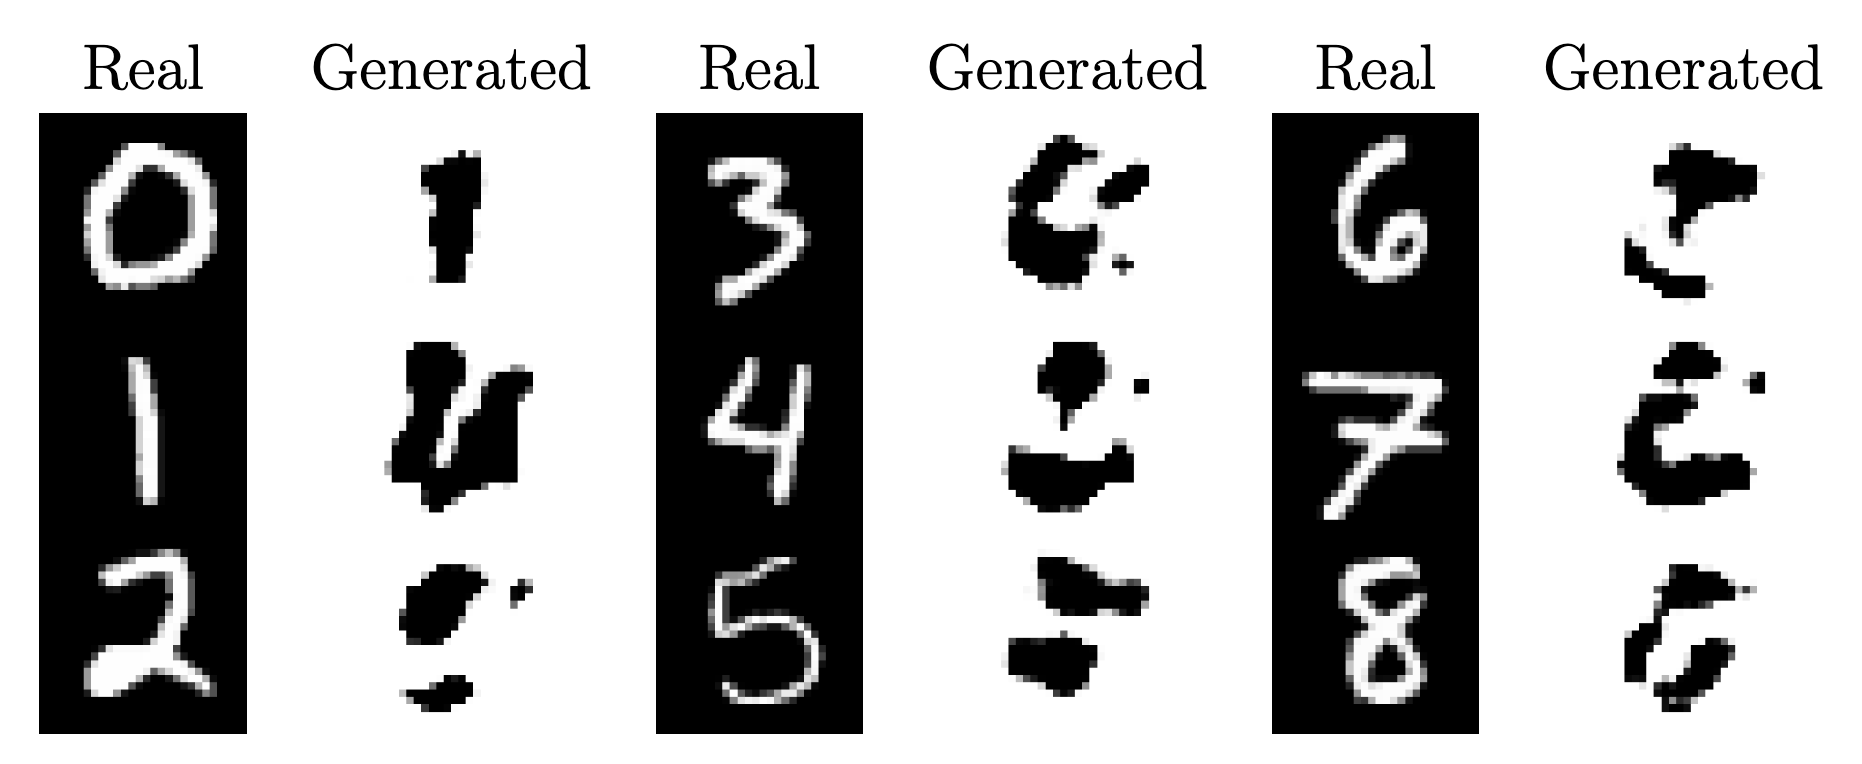
\includegraphics[width=\textwidth]{images/mnist_demo.png}
            \caption{Ілюстрація роботи генератора $\mathcal{G}$ на наборі данних \textit{MNIST}.}
        \end{figure}
    \end{frame}

    \begin{frame}{Приклади зображень. LFW}
        \begin{figure}
        \centering
            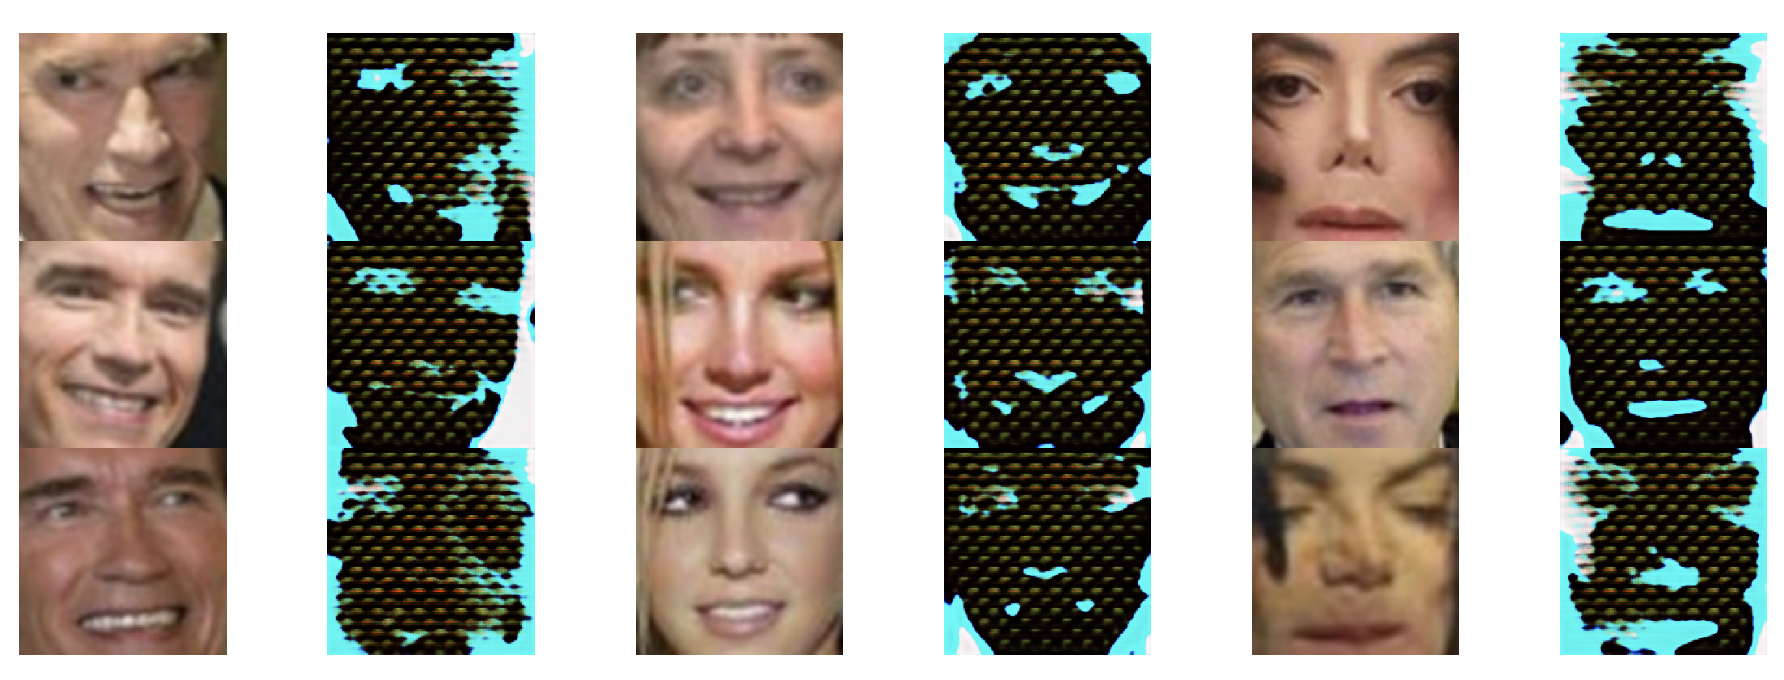
\includegraphics[width=\textwidth]{images/lfw_demo.png}
            \caption{Ілюстрація роботи генератора $\mathcal{G}$ на наборі данних \textit{LFW}.}
        \end{figure}
    \end{frame}

    \section{Генерація криптографічного ключа}

    \begin{frame}{Нечіткий екстрактор (Fuzzy Extractor).}
        Нечіткий екстрактор складається з двох функцій:
        \begin{itemize}
            \item $\mathsf{Gen}$ (generate) приймає строку $s \in \{0,1\}^{\ell}$ і видає шифр $r \in \{0,1\}^L$ з допоміжною строкою $p \in \{0,1\}^*$.
            \item $\mathsf{Rep}$ (reproduce) приймає строку $s' \in \{0,1\}^{\ell}$ та допоміжну строку $p \in \{0,1\}^*$, видає шифр $r' \in \{0,1\}^L$.
        \end{itemize}

        \textbf{Коректність.}
        \begin{equation*}
            \mathbb{P}\begin{bmatrix}
                r,p \gets \mathsf{Gen}(s) \\
                \mathsf{dist}(s,s') < t \\
                \mathsf{Rep}(s',p) = r
            \end{bmatrix} = 1 - \mathsf{negl}(\lambda)
        \end{equation*}

        \textit{На практиці} достатньо $t \approx \frac{\ell}{4}$.
    \end{frame}

    \begin{frame}{Нечіткий екстрактор для системи автентифікації.}
        \begin{figure}
        \centering
            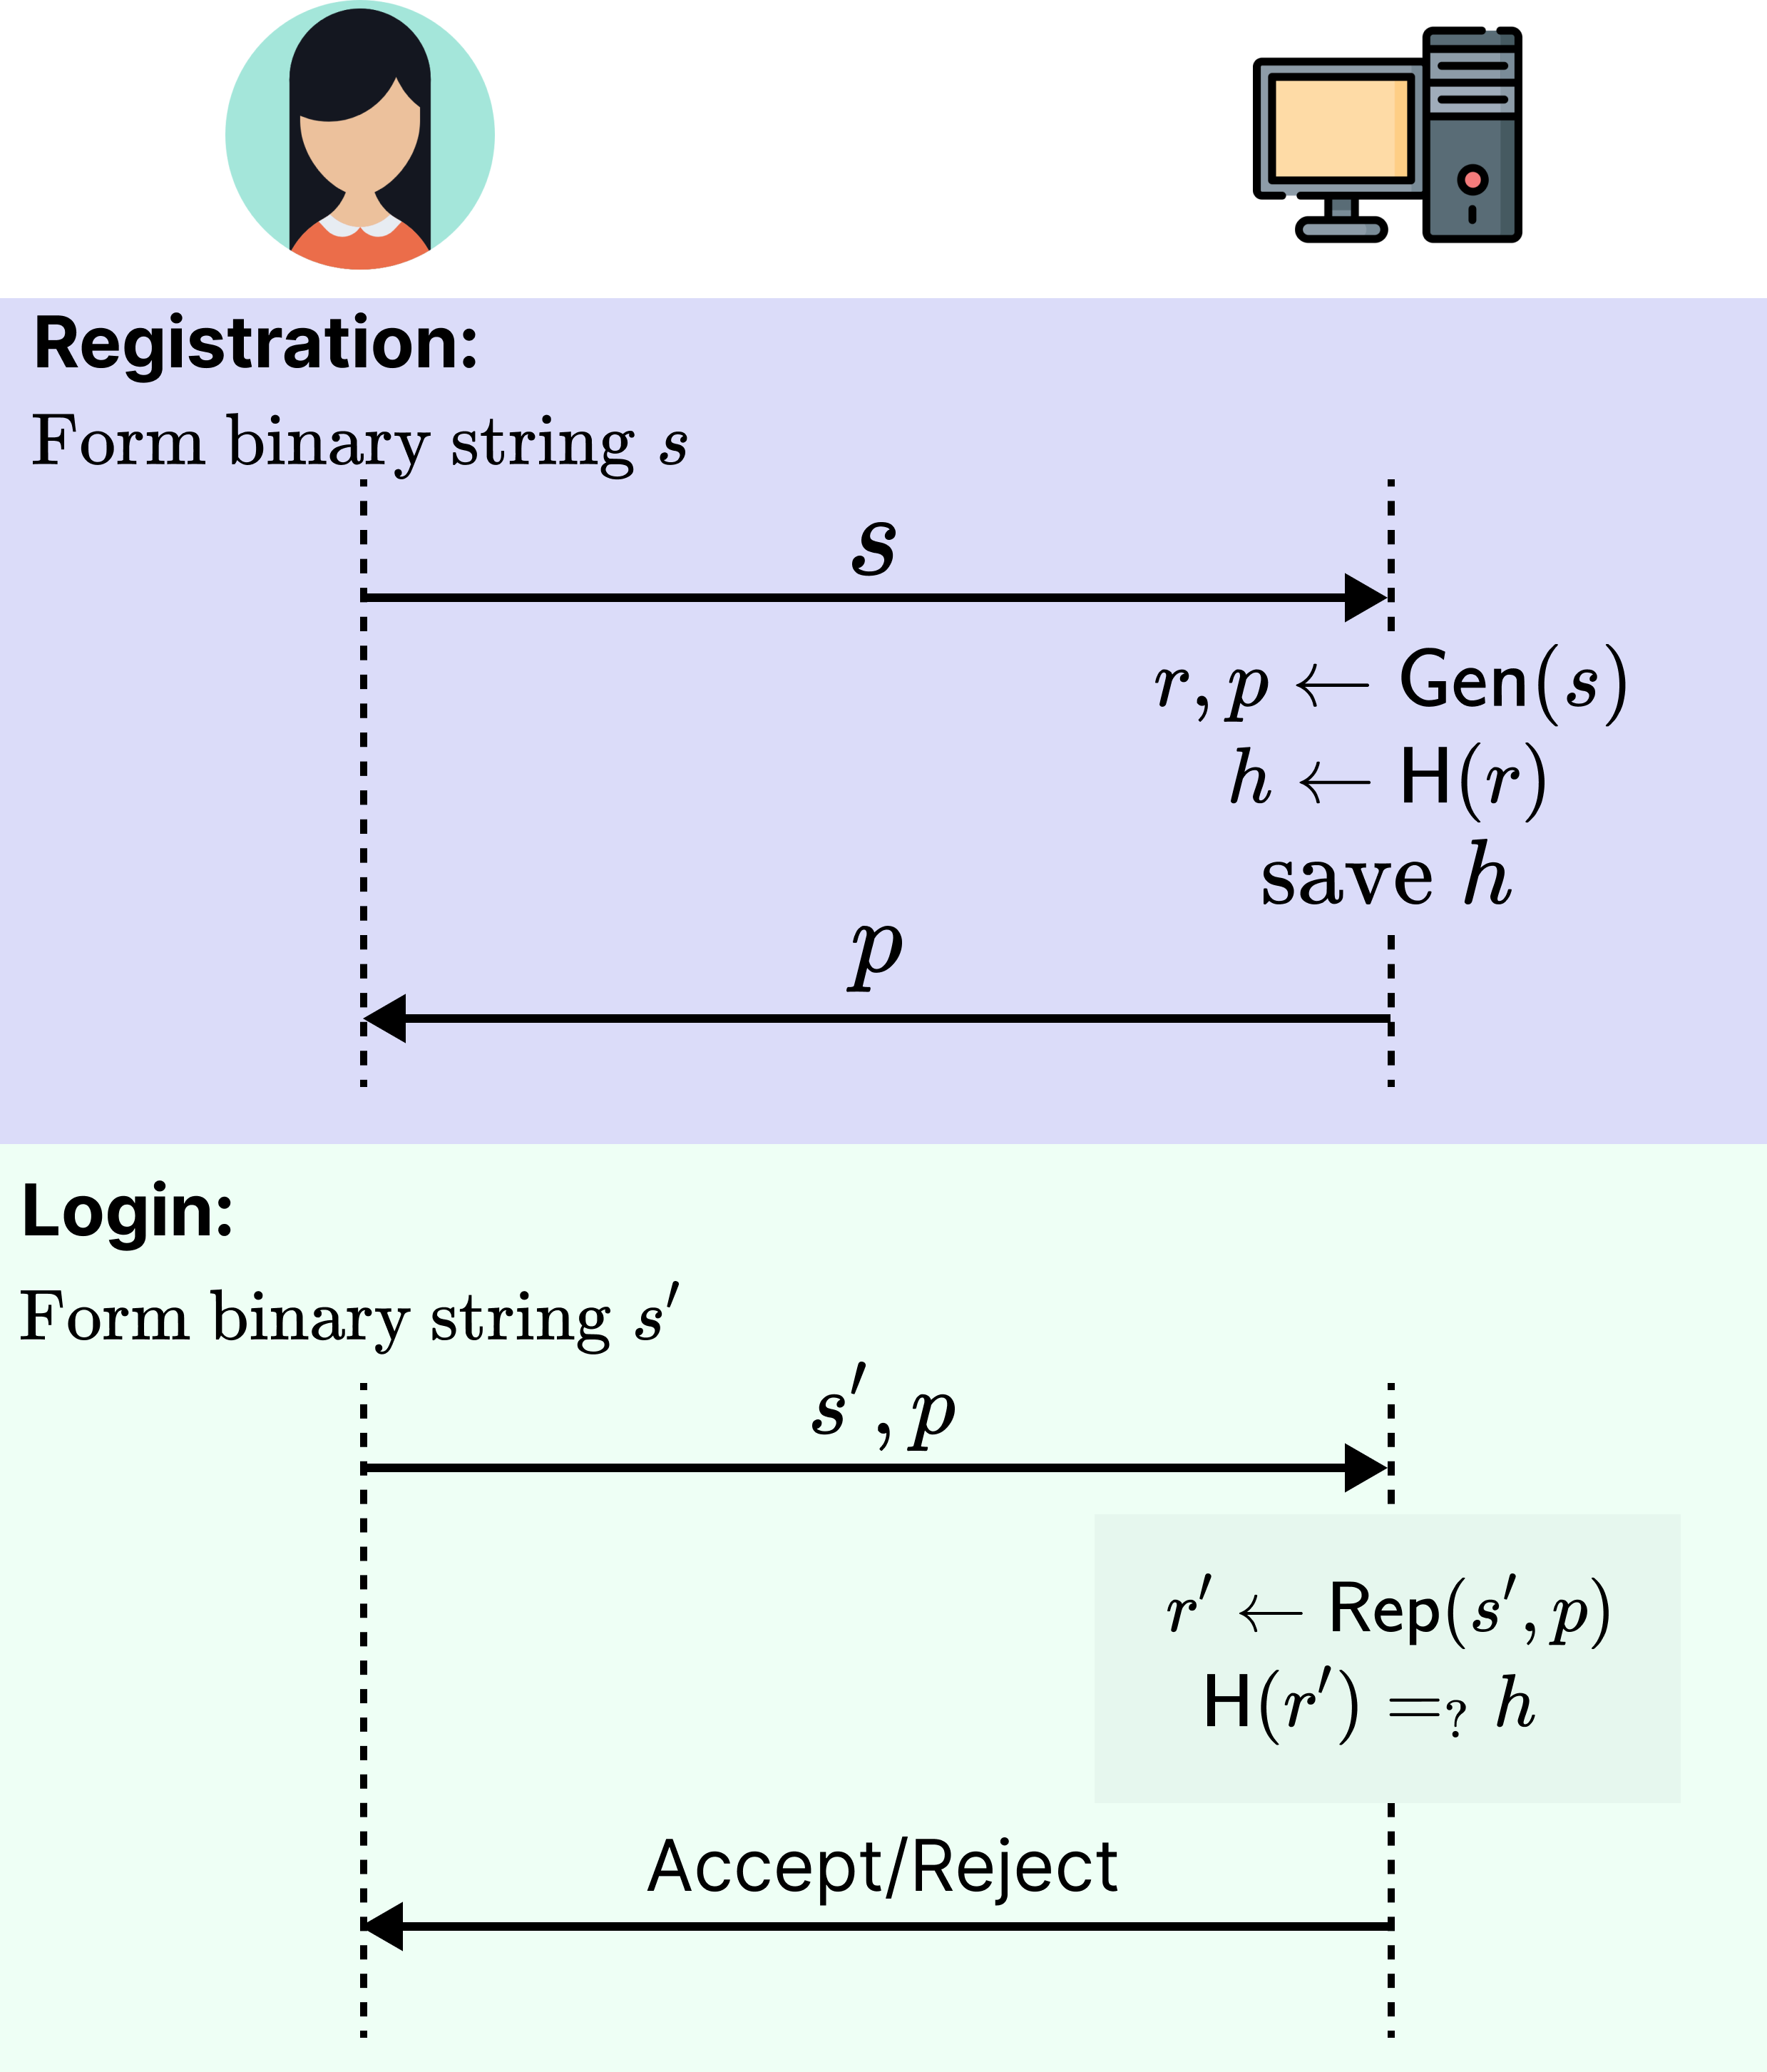
\includegraphics[width=0.55\textwidth]{images/fuzzy_auth.png}
        \end{figure}
    \end{frame}

    \begin{frame}{Бінарний екстрактор.}
        Задача нейронної мережі побудувати функцію $\phi: \mathsf{Image} \to \{0,1\}^{\ell}$.

        \begin{block}{Ідея \#1}
        Спочатку знайдемо ембедінги за допомогою FaceNet: $\mathcal{F}: \mathcal{I} \to \mathbb{R}^{\ell}$, а далі побудуємо $\mathbb{R}^{\ell} \mapsto \{0,1\}^{\ell}$.
        \end{block}

        \begin{block}{Ідея \#2}
        Візьмемо знак $\mathcal{F}_i(X),i \in [\ell]$ для отримання бінарної строки: $\phi(X) = \mathsf{Sign}\left(\mathcal{F}(X) > \boldsymbol{0}\right)$.
        \end{block}

        \begin{block}{Ідея \#3}
        Будемо брати знак відносно $\boldsymbol{\mu} := \mathbb{E}_{X \sim p_{\text{data}}}[\mathcal{F}(X)]$: $\phi(X) = \mathsf{Sign}\left(\mathcal{F}(X) > \boldsymbol{\mu}\right)$.
        \end{block}
    \end{frame}

    \begin{frame}{Результати.}
        Середня схожість однакових людей -- $75\%$, 
        
        Середня схожість різних людей -- $50\%$.
        \begin{figure}
        \centering
            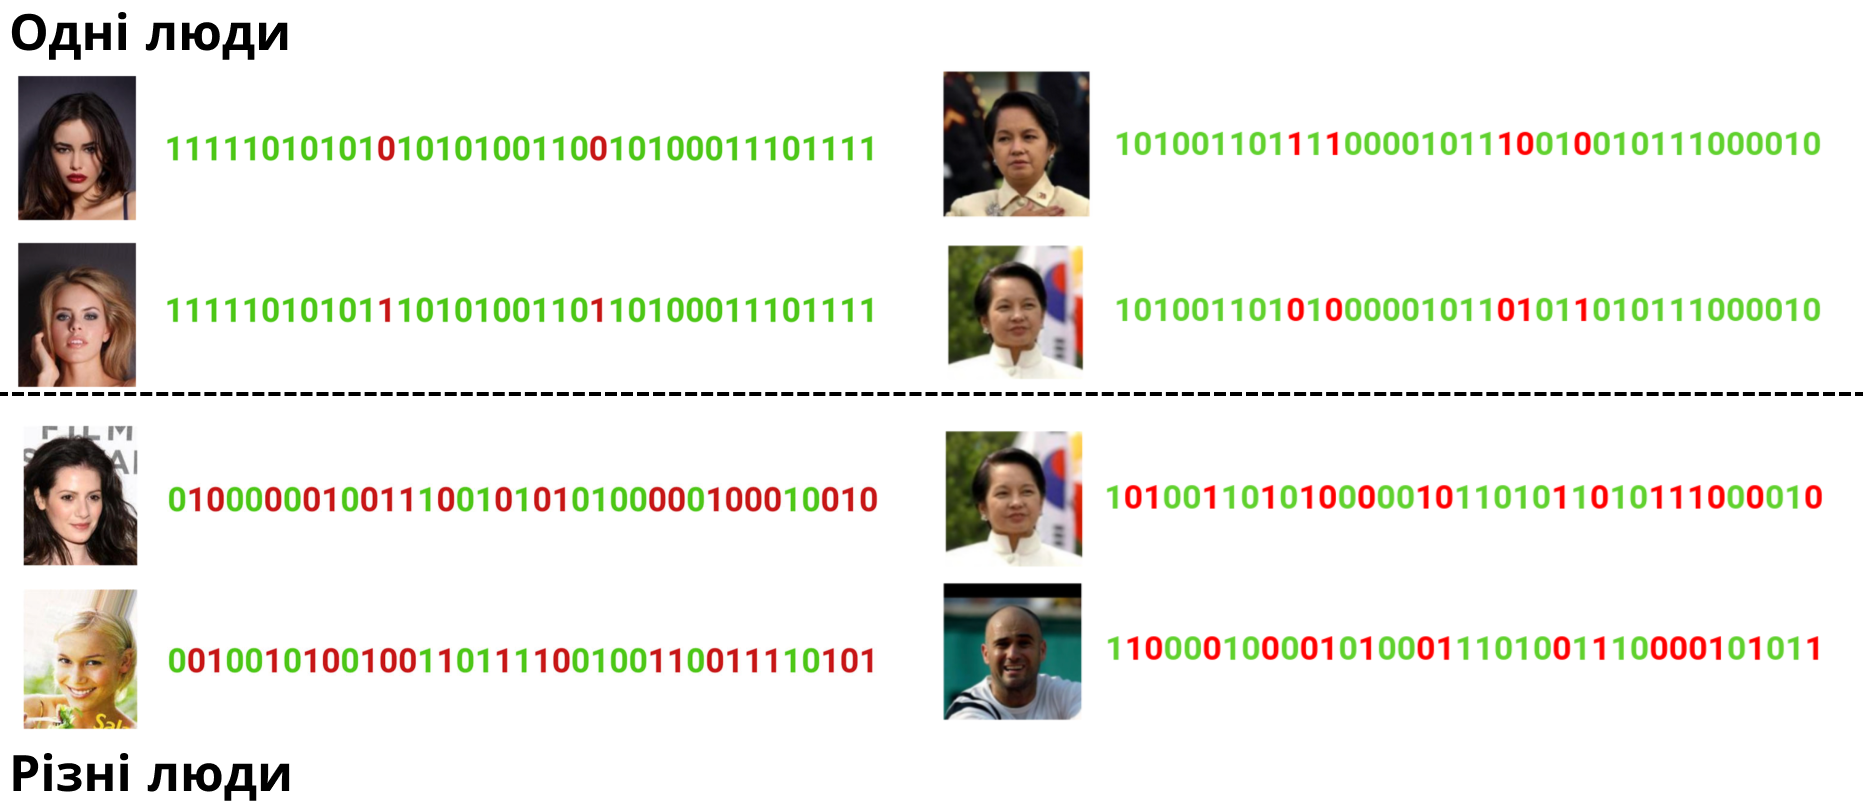
\includegraphics[width=\textwidth]{images/fuzzy_res.png}
            \caption{Ілюстрація роботи конвертатора у бінарну строку.}
        \end{figure}
    \end{frame}

    \section{Детекція живності}

    \begin{frame}{Формулювання}
        \begin{figure}
        \centering
            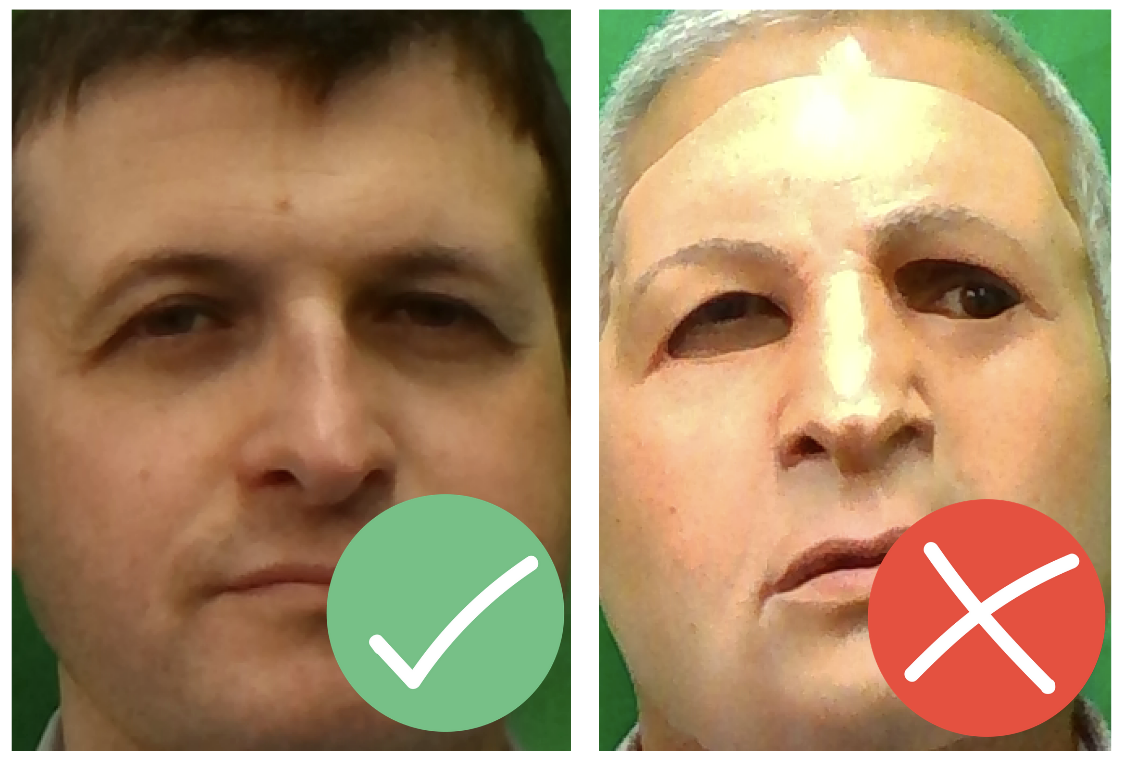
\includegraphics[width=0.6\textwidth]{images/statement.png}
            \caption{Постановка задачі. Спираючись на зображення $X \in \mathcal{I}$, видати ймовірність того, що перед нами нереальна людина.}
        \end{figure}
    \end{frame}

    \begin{frame}{Архітектура}
        \begin{figure}
        \centering
            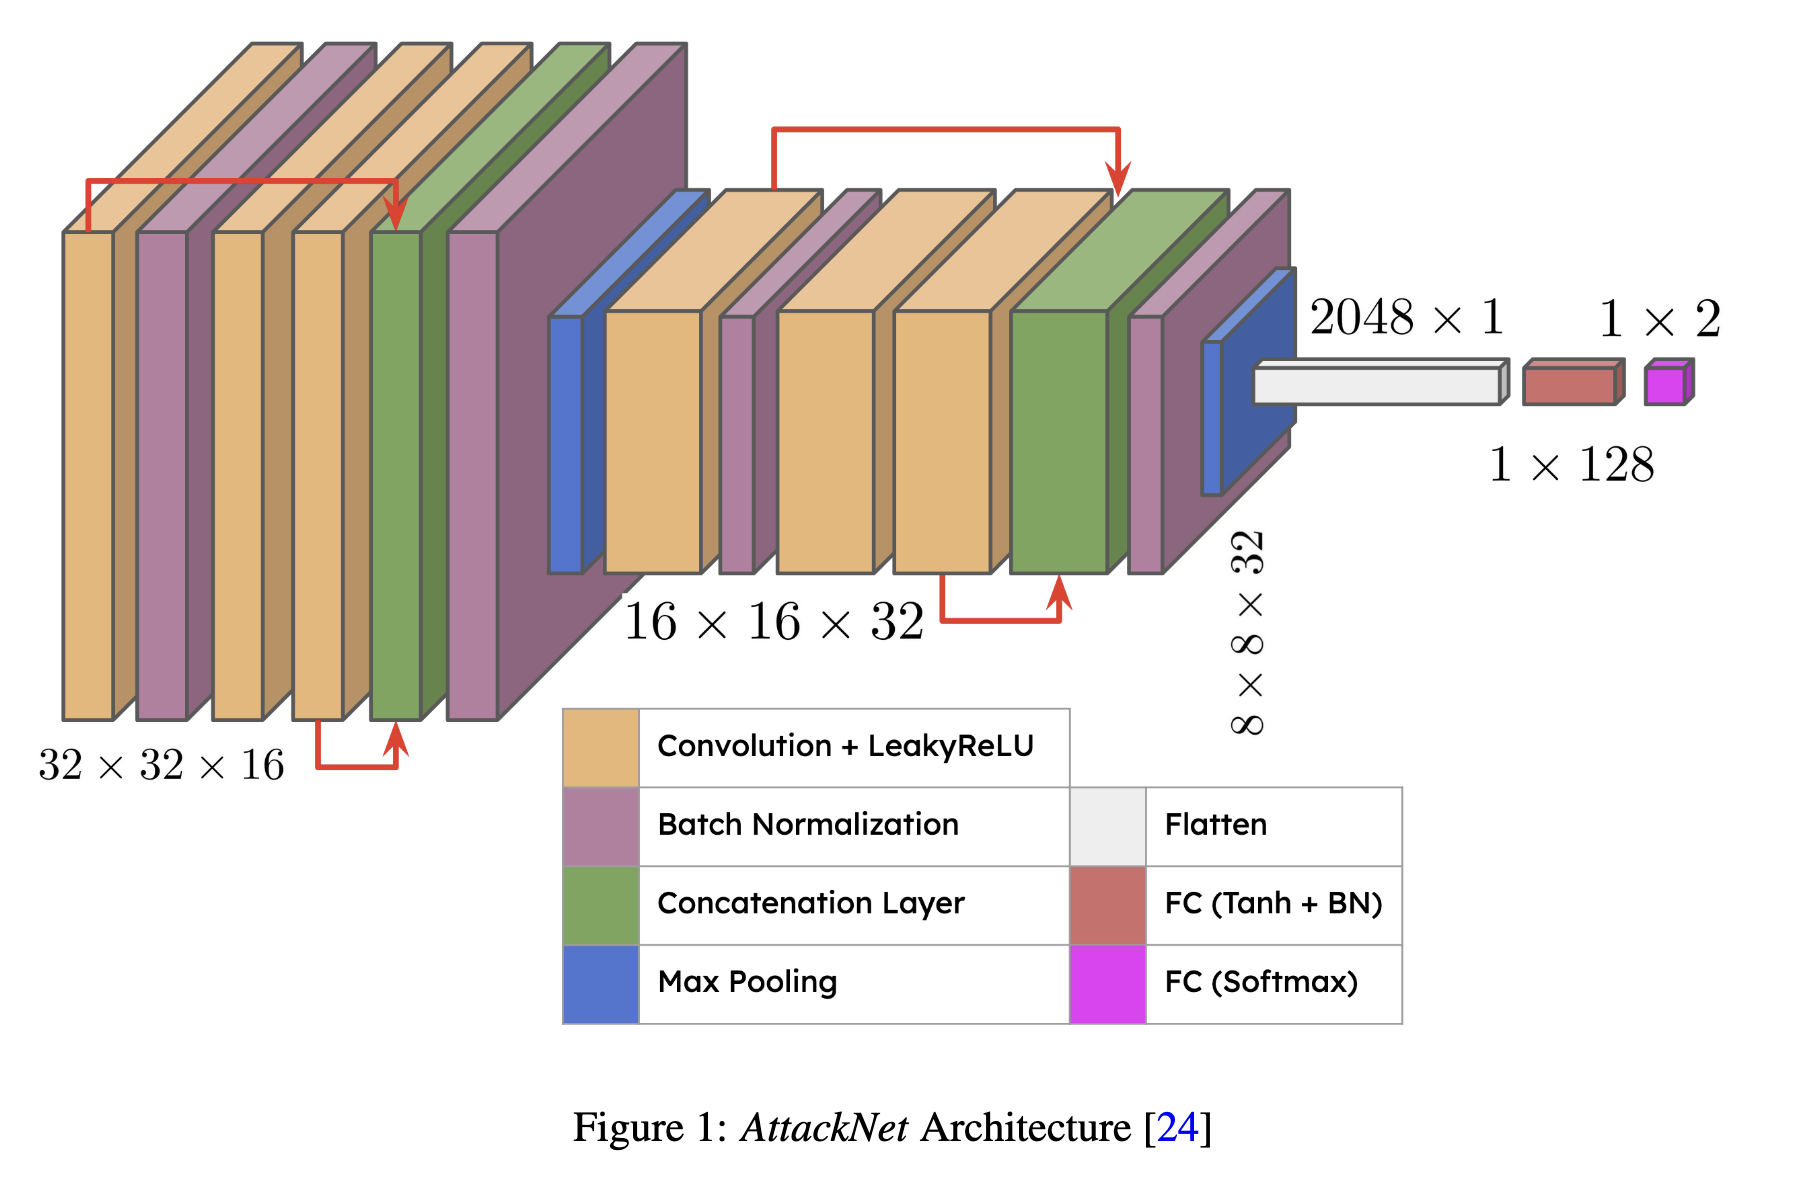
\includegraphics[width=0.8\textwidth]{images/attacknet.png}
            \caption{Архітектура \textit{AttackNet v2.2}.}
        \end{figure}
    \end{frame}

    \begin{frame}{Набори данних}
        \begin{figure}
        \centering
            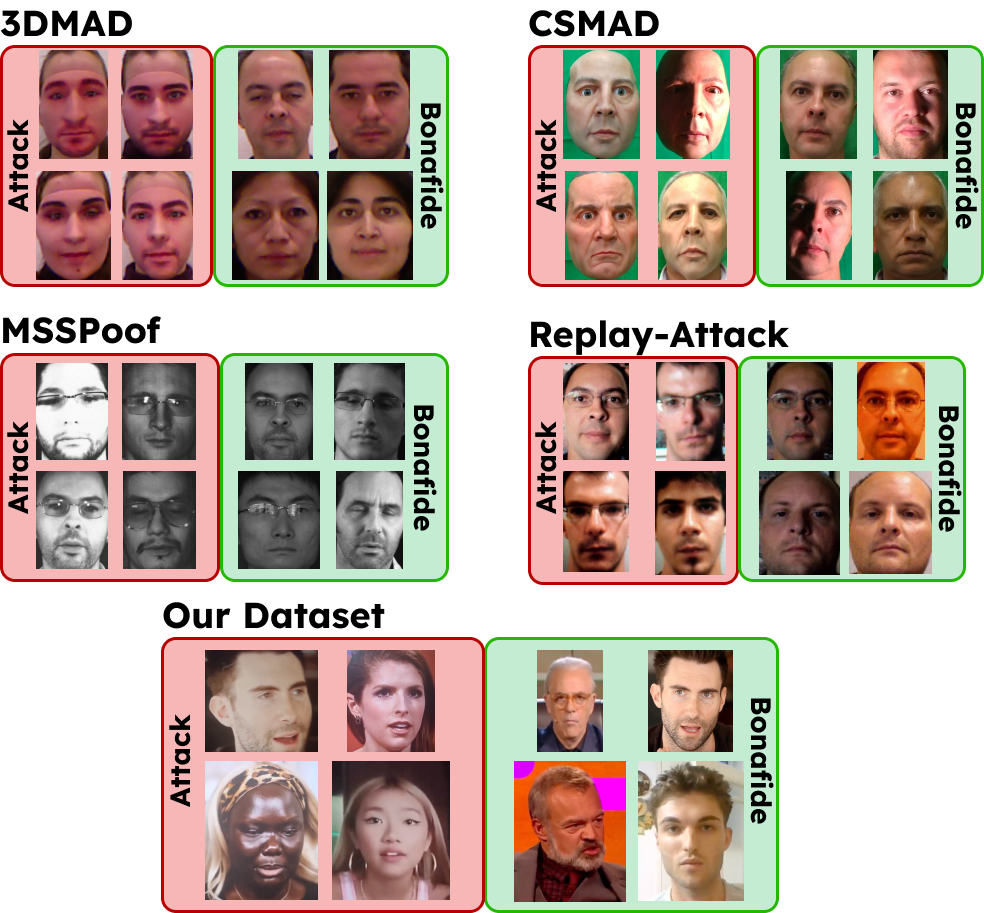
\includegraphics[width=0.6\textwidth]{images/anti_datasets.png}
            \caption{Набори данних, на яких проводилось тренування.}
        \end{figure}
    \end{frame}

    \begin{frame}{Attention Maps}
        \begin{figure}
        \centering
            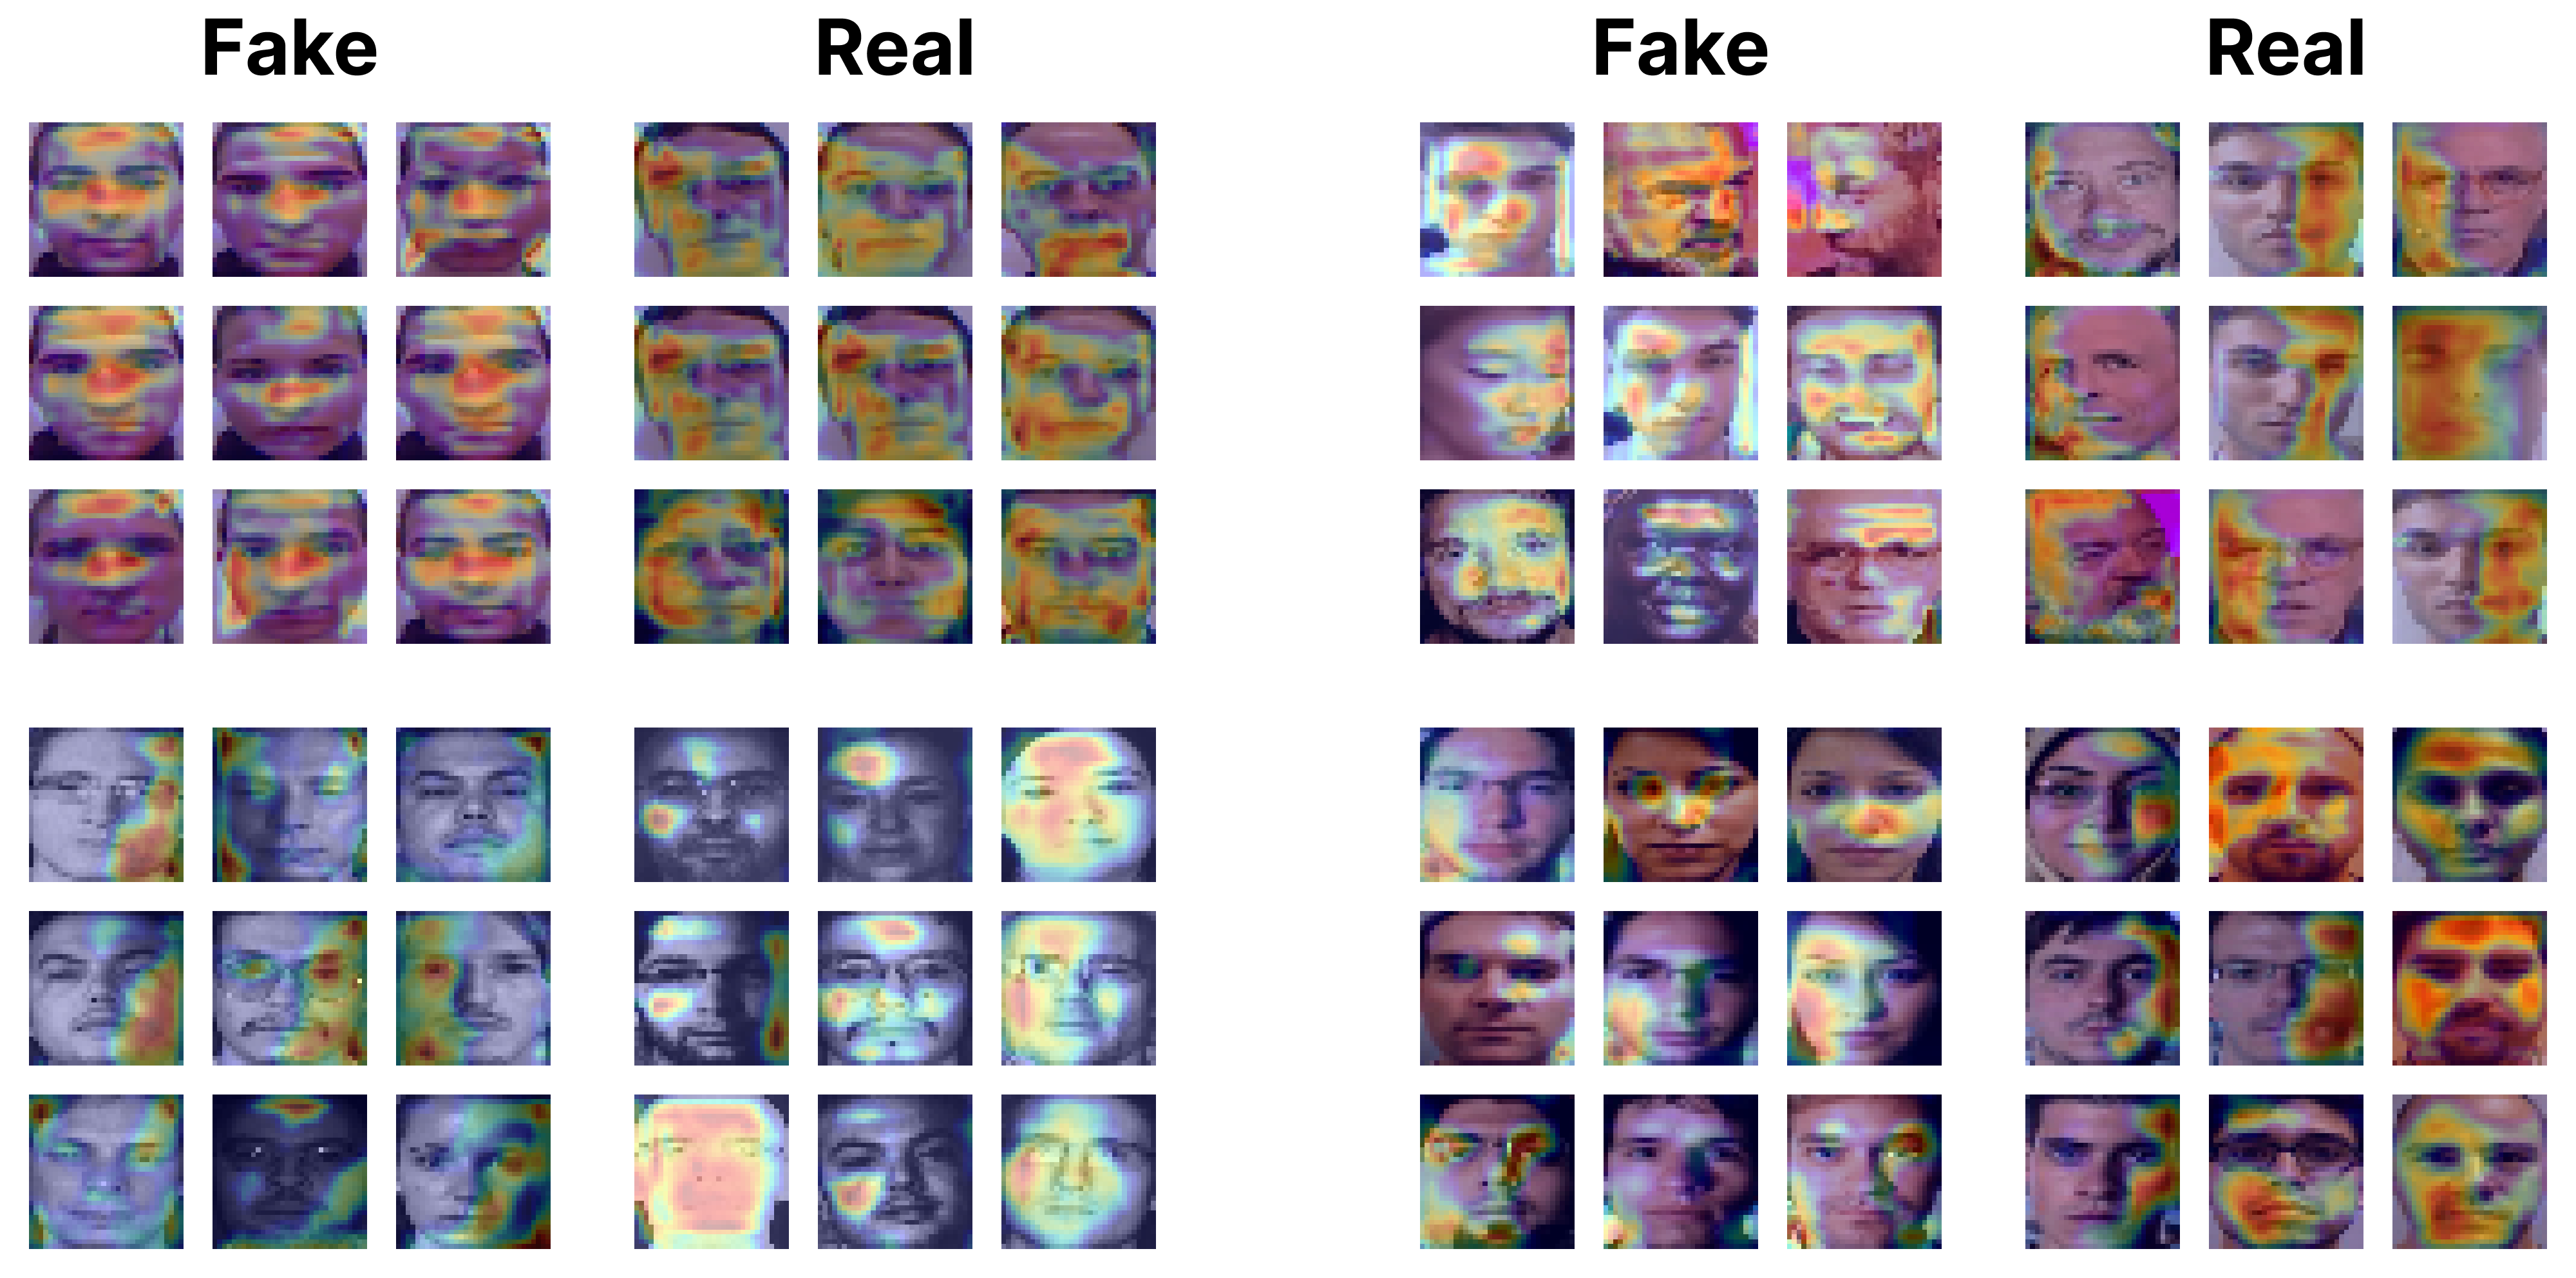
\includegraphics[width=\textwidth]{images/maps.png}
            \caption{Які зони облич нейронна мережа вважає важливими?}
        \end{figure}
    \end{frame}

    \begin{frame}{Найбільш актуальні напрямки досліджень}
        \begin{itemize}
            \item Мультибіометрія.
            \item Наскільки безпечно використовувати генератор $\mathcal{G}$? Ввести формальне поняття безпеки біометрії в контексті некриптографічно стійких систем.
            \item Аналог гомоморфного шифрування: чи можна, маючи зашифрований шаблон $\mathcal{G}(X)$, зробити висновки по ньому?
            \item Перевести обрахунки над $\mathbb{R}$ в операції над скіченними полями $\mathbb{F}_p$: двері до \textit{zero-knowledge proofs} (або zkml).
        \end{itemize}
    \end{frame}
    
	\begin{frame}{}
      \centering \Large
      \emph{Дякую за увагу!}
    \end{frame}

\end{document}
